\chapter{Surgery Theory}
    \section{A Review of Topology}
        \subsection{Homotopy}
            From Topology, a continuous function from a topological space $X$
            to a topological space $Y$ is a function $f:X\rightarrow{Y}$ such
            that for all open subsets $\mathcal{U}\subseteq{Y}$, the pre-image
            $f^{-1}(\mathcal{U})$ is an open subset of $X$.
            \begin{fnotation}{}{}
                The set of continuous functions $f:{X}\rightarrow{Y}$
                is denoted $C(X,Y)$.
            \end{fnotation}
            Let $X$ and $Y$ be topological spaces, and let
            $f:{X}\rightarrow{Y}$ and $g:{X}\rightarrow{Y}$ be continuous
            functions. Let $I$ denote the closed unit interval $[0,1]$. We now
            define what it means for $f$ and $g$ to be \textit{homotopic}.
            \begin{ldefinition}{Homotopy}{Homotopy}
                A homotopy between continuous functions
                $f,g:{X}\rightarrow{Y}$ is a continuous function
                $H:{X}\times{I}\rightarrow{Y}$ such that $H(x,0)=f(x)$ and
                $H(x,1)=g(x)$.
            \end{ldefinition}
            \begin{figure}[H]
                \centering
                \captionsetup{type=figure}
                \documentclass[crop,class=article]{standalone}
%----------------------------Preamble-------------------------------%
\usepackage{tikz}                       % Drawing/graphing tools.
\usetikzlibrary{arrows.meta}            % Latex and Stealth arrows.
%--------------------------Main Document----------------------------%
\begin{document}
    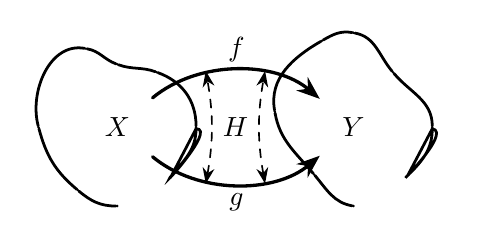
\begin{tikzpicture}[%
        line width=1pt,
        line cap=round,>={Stealth[black]},
        every edge/.style={draw=black,very thick},
        smalldot/.style={
            circle,
            fill=black,
            inner sep=0pt,
            outer sep=0
        }
    ]
        \begin{scope}[every node/.style=smalldot]
            % Set points defining the leftmost blob.
            \node at (0,0) (a) {};
            \node at (-0.5,0.2) (b) {};
            \node at (-1,1) (c) {};
            \node at (-0.4,2) (d) {};
            \node at (0, 1.8) (e) {};
            \node at (0.5, 1.7) (f) {};
            \node at (1,1) (g) {};
            \node at (0.7,0.4) (h) {};

            % Set points defining the rightmost blob.
            \node at (3,0) (a1) {};
            \node at (2.5,0.4) (b1) {};
            \node at (2,1.2) (c1) {};
            \node at (2.6,2.1) (d1) {};
            \node at (3, 2.2) (e1) {};
            \node at (3.5, 1.7) (f1) {};
            \node at (4,1) (g1) {};
            \node at (3.7,0.4) (h1) {};
        \end{scope}

        % Labels for the blobs X and Y.
        \node at (0,1) (i) {$X$};
        \node at (3,1) (i1) {$Y$};

        % Node indicating this is a homotopy.
        \node at (1.5,1) (ho) {$H$};

        % Nodes for drawing arrows between curves.
        \node at (1.1,0.15) (t1) {};
        \node at (1.1,1.85) (t2) {};
        \node at (1.9,0.15) (t3) {};
        \node at (1.9,1.85) (t4) {};

        % Draw a Hobby curve creating leftmost blob.
        \draw (a) to [out=180,in=-40] (b)
                  to [out=140,in=-75] (c)
                  to [out=105,in=170] (d)
                  to [out=-10,in=160] (e)
                  to [out=-20,in=160] (f)
                  to [out=-20,in=90] (g)
                  to [out=-90,in=50] (h)
                  to [out=-130,in=0] cycle;

        % Draw Hobby curve creating rightmost blob.
        \draw (a1) to [out=170,in=-50] (b1)
                   to [out=130,in=-80] (c1)
                   to [out=100,in=-150] (d1)
                   to [out=30,in=170] (e1)
                   to [out=-10,in=130] (f1)
                   to [out=-50,in=90] (g1)
                   to [out=-90,in=45] (h1)
                   to [out=-135,in=-10] cycle;

        % Draw arrows representing f and g.
        \path[shorten >=0.2cm,shorten <=0.2cm,->]
            (i) edge[bend left=40] node[above] {$f$} (i1);
        \path[shorten >=0.2cm,shorten <=0.2cm,->]
            (i) edge[bend right=40] node[below] {$g$} (i1);

        % Draw first arrow connecting f and g.
        \path[draw=black,dashed,<->]
            (t1) edge[bend right =10,semithick] (t2);

        % Draw second arrow connecting f and g.
        \path[draw=black,dashed,<->]
            (t3) edge[bend left =10,semithick] (t4);
    \end{tikzpicture}
\end{document}
                \caption{Homotopy Between Two Functions}
                \label{fig:homotopy_diagram_for_depicting_homotopy}
            \end{figure}
            \begin{ldefinition}{Homotopic Functions}{Homotopic_Functions}
                Homotopic functions are continuous functions
                $f,g:{X}\rightarrow{Y}$, denoted ${f}\simeq{g}$,
                such that there exists a homotopy between them.
            \end{ldefinition}
            \begin{lexample}{Straight Line Homotopy}{Straight_Line_Homotopy}
                Fig.~\ref{fig:homotopy_diagram_for_depicting_homotopy} shows
                two topological spaces and two homotopic continuous functions.
                For a more concrete example, let
                $f,g:\mathbb{R}^{n}\rightarrow\mathbb{R}^{m}$ be continuous.
                The \textit{straight-line} homotopy is a homotopy between such
                functions. Define
                $H:\mathbb{R}^{n}\times{I}\rightarrow\mathbb{R}^{m}$ by:
                \begin{equation}
                    \label{eqn:Straight_Line_Homotopy}
                    H(x,t)=(1-t)f(x)+tg(x)
                \end{equation}
                Then $H(x,0)=f(x)$, $H(x,1)=g(x)$, and $H$ is continuous. Thus,
                ${f}\simeq{g}$. Note that $g(x)=constant$ is possible. Any
                continuous function $f:\mathbb{R}^{n}\rightarrow\mathbb{R}^{m}$
                is homotopic to a point.
            \end{lexample}
            We can visualize homotopy by letting $X=I$ and
            $Y\subset\mathbb{R}^{2}$ be a nice blob, like the one shown in
            Fig.~\ref{fig:straight_line_homotopy}. Let
            $f,g:[0,1]\rightarrow Y$ be smooth curves within the blob. Then
            the homotopy defined in Eqn.~\ref{eqn:Straight_Line_Homotopy} is
            the map that drags $f(x)$ to $g(x)$ via the straight line
            connecting the two points. This is done for every point
            $x\in [0,1]$.
            \begin{figure}[H]
                \centering
                \captionsetup{type=figure}
                \documentclass[crop,class=article]{standalone}
%----------------------------Preamble-------------------------------%
\usepackage{tikz}                       % Drawing/graphing tools.
\usetikzlibrary{arrows.meta}            % Latex and Stealth arrows.
%--------------------------Main Document----------------------------%
\begin{document}
    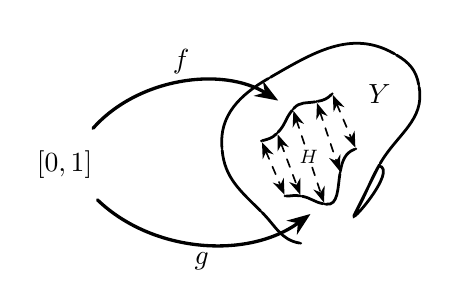
\begin{tikzpicture}[%
        line width=1pt,
        line cap=round,
        >={Stealth[black]},
        every edge/.style={draw=black,very thick},
        smalldot/.style={
            circle,
            fill=black,
            inner sep=0pt,
            outer sep=0
        },
        dashcurve/.style={
            draw=black,
            dashed,
            <->
        }
    ]
        \begin{scope}[every node/.style=smalldot]
            % Set points for upper curve.
            \node at (2.5,1.3) (a0) {};
            \node at (2.7,1.4) (b0) {};
            \node at (2.9,1.7) (c0) {};
            \node at (3.2,1.8) (d0) {};
            \node at (3.4,1.9) (e0) {};

            % Set points for lower curve.
            \node at (2.8,0.6) (a1) {};
            \node at (3,0.6) (b1) {};
            \node at (3.3,0.5) (c1) {};
            \node at (3.5,0.9) (d1) {};
            \node at (3.7,1.2) (e1) {};

            % Points for the outer blob.
            \node at (3,0) (a2) {};
            \node at (2.5,0.4) (b2) {};
            \node at (2,1.2) (c2) {};
            \node at (2.6,2.1) (d2) {};
            \node at (4.2, 2.4) (e2) {};
            \node at (4.5, 2) (f2) {};
            \node at (4,1) (g2) {};
            \node at (3.7,0.4) (h2) {};
        \end{scope}

        % Nodes labelling the domain and co-domain.
        \node at (0,1) (i) {$[0,1]$};
        \node at (4,1.9) (i1) {$Y$};

        % Draw upper curve.
        \draw (a0) to [out=15,in=-135] (b0)
                   to [out=45,in=-130] (c0)
                   to [out=50,in=-170] (d0)
                   to [out=10,in=-135] (e0);

        % Draw lower curve.
        \draw (a1) to [out=0,in=170] (b1)
                   to [out=-10,in=170] (c1)
                   to [out=-10,in=-100] (d1)
                   to [out=80,in=-160] (e1);

        \begin{scope}[%
            every path/.style=dashcurve,
            every edge/.style=semithick
        ]
            % Draw dashed lines connecting curves.
            \path (a0) edge (a1);
            \path (b0) edge (b1);
            \path (c0) edge
                node[inner sep=0pt,outer sep=0pt,fill=white]
                {\scriptsize{\textit{H}}} (c1);
            \path (d0) edge (d1);
            \path (e0) edge (e1);
        \end{scope}

        % Draw curve defining the blob.
        \draw (a2) to [out=170,in=-45] (b2)
                   to [out=135,in=-85] (c2)
                   to [out=95,in=-150] (d2)
                   to [out=30,in=150] (e2)
                   to [out=-30,in=100] (f2)
                   to [out=-80,in=60] (g2)
                   to [out=-120,in=60] (h2)
                   to [out=-120,in=-10] cycle;


        % Draw curves representing maps f and g.
        \path[shorten >=0.2cm,shorten <=0.2cm,->]
            (i) edge[bend left=40]
            node[above] {$f$} (c0);
        \path[shorten >=0.2cm,shorten <=0.2cm,->]
            (i) edge[bend right=40]
            node[below] {$g$} (c1);
    \end{tikzpicture}
\end{document}
                \caption{Straight-Line Homotopy.}
                \label{fig:straight_line_homotopy}
            \end{figure}
            The next thing to show is that the notion of homotopy $\simeq$
            is an equivalence relation on the set $C(X,Y)$.
            \begin{theorem}
                Homotopic is an equivalence relation.
            \end{theorem}
            \begin{proof}
                We must show that $\simeq$ is reflexive, symmetric, and
                transitive.
                \begin{enumerate}
                    \item If ${f}\in{C(X,Y)}$, let $H(x,t)=f(x)$. Then
                          $H\in{C({X}\times{I},Y)}$, $H(x,0)=f(x)$,
                          and $H(x,1)=f(x)$. Thus $H$ is a homotopy between
                          $f$ and itself so $f\simeq f$.
                    \item If ${f,g}\in{C(X,Y)}$ and ${f}\simeq{g}$, then there
                          exists a homotopy $H$ between $f$ and $g$. Let
                          $G=H(x,1-t)$. Then, since the composition of
                          continuous functions is continuous,
                          $G\in{C({X}\times{I},Y)}$. But also $G(x,0)=g(x)$ and
                          $G(x,1)=f(x)$. Therefore, ${g}\simeq{f}$.
                    \item If ${f,g,h}\in{C(X,Y)}$, ${f}\simeq{g}$, and
                          ${g}\simeq{h}$, then there exist a homotopy $H_{1}$
                          between $f$ and $g$ and a homotopy $H_{2}$ between
                          $g$ and $h$. Let $H:{X}\times{I}\rightarrow{Y}$
                          be defined by:
                          \begin{equation}
                              H(x,t)=
                              \begin{cases}
                                  H_{1}(x,2t),&{0}\leq{t}\leq\frac{1}{2}\\
                                  H_{2}(x,2t-1),&\frac{1}{2}<{t}\leq{1}
                              \end{cases}
                          \end{equation}
                          By the pasting lemma, $H\in{C({X}\times{I},Y)}$.
                          But from the definition of $H_{1}$ and $H_{2}$,
                          $H(x,0)=f(x)$ and $H(x,1)=h(x)$. Thus, $f\simeq{h}$.
                \end{enumerate}
                Thus homotopic forms an equivalence relation.
            \end{proof}
            \begin{ldefinition}{Homotopy Inverse}{Homotopy_Inverse}
                A homotopy inverse of a function $f\in{C}(X,Y)$ is a function
                $g\in{C}(Y,X)$ such that $g\circ{f}\simeq{id}_{X}$ and
                $f\circ{g}\simeq{id}_{Y}$.
            \end{ldefinition}
            \begin{theorem}
                If $X$ and $Y$ are topological spaces, $f:X\rightarrow{Y}$ is
                continuous, and if $g_{1}$ and $g_{2}$ are homotopy inverses
                of $f$, then $g_{1}\simeq{g}_{2}$.
            \end{theorem}
            \begin{proof}
                Since $g_{2}$ is a homotopy inverse of $f$,
                $f\circ{g}_{2}\simeq{id}_{Y}$. But then:
                \begin{equation}
                    g_{1}\simeq{g}_{1}\circ(f\circ{g}_{2})
                    =(g_{1}\circ{f})\circ{g}_{2}
                \end{equation}
                But $g_{1}$ is a homotopy of inverse of $f$,
                and thus $g_{1}\circ{f}\simeq{id}_{X}$. Thus:
                \begin{equation}
                    (g_{1}\circ{f})\circ{g}_{2}\simeq{g}_{2}
                \end{equation}
                Therefore, as homotopic is a transitive relation,
                $g_{1}\simeq{g}_{2}$.
            \end{proof}
            \begin{ldefinition}{Homotopy Equivalence}{Homotopy_Equivalence}
                A homotopy equivalence from a topological space $X$ to a
                topological space $Y$ is a function $f\in{C}(X,Y)$ such that
                there exists a homotopy inverse $g$ of $f$.
            \end{ldefinition}
            \begin{ldefinition}{Homotopy Equivalent Spaces}
                               {Homotopy_Equivalent_Spaces}
                Homotopy equivalent spaces are topological spaces $X$ and $Y$
                such that there exists functions ${f}\in{C(X,Y)}$ and
                ${g}\in{C(Y,X)}$ such that ${f}\circ{g}\simeq{id_{Y}}$
                and ${g}\circ{f}\simeq{id_{X}}$.
            \end{ldefinition}
            From the definition of homotopy equivalent spaces it is important
            to note that it is not required that $g\circ{f}=id_{X}$, but rather
            that $g\circ{f}$ is \textit{homotopic} to the identity map $id_{X}$.
            Similarly, $f\circ{g}$ need only be homotopic to the identity map
            $id_{Y}$, and not equal to it. We can rephrase this by saying that
            homotopy equivalent spaces are topological spaces $X$ and $Y$ such
            that there exists a homotopy equivalence $f:X\rightarrow{Y}$
            between the two. There is a stronger notion between topological
            spaces called \textit{homeomorphisms}.
            \begin{ldefinition}{Homeomorphism}{Homeomorphism}
                A homeomorphism from a topological space $X$ to a topological
                space $Y$ is a continuous bijection $f:{X}\rightarrow{Y}$ such
                that $f^{-1}:{Y}\rightarrow{X}$ is continuous.
            \end{ldefinition}
            \begin{ldefinition}{Homeomorphic Topological Spaces}
                               {Homeomorphic_Topological_Spaces}
                Homeomorphic topological spaces are topological spaces $X$
                and $Y$ such that there exists a homeomorphism
                $f:{X}\rightarrow{Y}$ between them.
            \end{ldefinition}
            \begin{ltheorem}{Homeomorphic Implies Homotopy Equivalent}
                            {Homeomorphic_Implies_Homotopy_Equivalent}
                If $X$ and $Y$ are homeomorphic,
                then they are homotopy equivalent.
            \end{ltheorem}
            \begin{proof}
                If $X$ and $Y$ are homeomorphic topological spaces, then there
                is a homeomorphism $f:X\rightarrow Y$. But then $f$ is a
                continuous map from $X$ to $Y$, and $f^{-1}$ is a continuous
                map from $Y$ to $X$. Moreover, ${f}\circ{f^{-1}}=id_{Y}$, and
                ${f^{-1}}\circ{f}=id_{X}$, for $f$ is a bijection. But
                ${id_{X}}\simeq{id_{X}}$, and ${id_{Y}}\simeq{id_{Y}}$.
                Therefore, etc.
            \end{proof}
            The study of surgery theory asks about the
            converse of Thm.~\ref{thm:Homeomorphic_Implies_Homotopy_Equivalent}.
            The converse of this theorem is not always true,as we will now
            demonstrate.
            \begin{theorem}
                \label{thm:homotopic_does_not_imply_homeomorphic}%
                There exist topological spaces that are
                homotopy equivalent but not homeomorphic.
            \end{theorem}
            \begin{proof}
                Let $X=\mathbb{R}^{2}$ and $Y=\{(0,0)\}$.
                Let $f:{X}\rightarrow{Y}$ be defined by
                $f(x,y)=(0,0)$ and $g=id_{Y}$. Then
                $g\circ{f}=(0,0)$. Let $H(x,y,t)=(1-t)(x,y)$.
                Then $H$ is continuous, $H(x,y,0)=(x,y)$,
                and $H(x,y,1)=(0,0)$. Thus, $H$ is a
                homotopy between ${g}\circ{f}$ and $id_{X}$, and
                therefore ${g}\circ{f}\simeq{id_{X}}$. But
                ${f}\circ{g}=id_{Y}$, and ${id_{Y}}\simeq{id_{Y}}$.
                Thus $X$ and $Y$ are homotopy equivalent.
                If $h:{X}\rightarrow{Y}$ is a homeomorphism, then it is a
                bijection. But then $\Card(X)=\Card(Y)$,
                where $\Card$ denotes the \textit{cardinality} of the space.
                But $\mathbb{R}^{2}$ is uncountable, and $\Card(Y)=1$,
                a contradiction. Therefore $X$ and $Y$ are not homeomorphic.
            \end{proof}
            \begin{figure}[H]
                \captionsetup{type=figure}
                \centering
                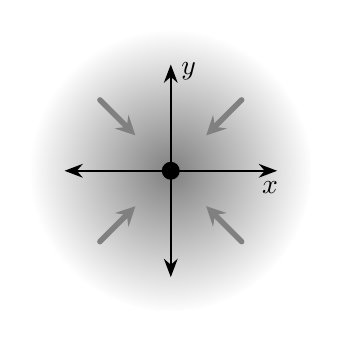
\begin{tikzpicture}[%
    scale=0.9,
    line width=1pt,
    line cap=round,
    >={Stealth[black]},
    every edge/.style={%
        draw=black,
        very thick
    },
    grayarrow/.style={%
        >=stealth,
        fill=gray,
        draw=gray,
        line width=0.7mm,
        ->
    }
]
    \filldraw[%
        even odd rule,
        inner color=gray,
        outer color=white,
        draw=white
    ] (0,0) circle (2);
    \draw[thick, <->] (-1.5,0)--(1.5,0);
    \draw[thick, <->] (0,-1.5)--(0,1.5);
    \draw[grayarrow] (1,1)--(0.5,0.5);
    \draw[grayarrow] (-1,-1)--(-0.5,-0.5);
    \draw[grayarrow] (1,-1)--(0.5,-0.5);
    \draw[grayarrow] (-1,1)--(-0.5,0.5);
    \node[%
        fill=black,
        circle,
        thick,
        draw,
        inner sep=2pt,
        outer sep=3pt
    ]
        at (0,0) (O) {};
    \node at (1.4,0) [below] {$x$};
    \node at (0,1.4) [right] {$y$};
\end{tikzpicture}
                \caption{Retraction of $\mathbb{R}^{2}$ to $(0,0)$}
                \label{fig:homotopy_equivalence_of_plane_with_point}
            \end{figure}
            Fig.~\ref{fig:homotopy_equivalence_of_plane_with_point}
            shows the mapping $f$ between $\mathbb{R}^{2}$ and $\{(0,0)\}$.
            Thm.~\ref{thm:homotopic_does_not_imply_homeomorphic} relies on the
            fact that $\mathbb{R}^{2}$ and $\{(0,0)\}$ are of different
            \textit{cardinality}. However, even if the topological spaces $X$
            and $Y$ are homotopy equivalent, and are of the same cardinality,
            it is still possible that they are not homeomorphic. We will need
            to show that homeomorphisms preserve the notion of
            \textit{compactness}.
            \begin{ldefinition}{Open Covers}{Open_Covers}
                An open cover of a subset $A$ of a topological space $X$ with
                topology $\tau$ is a set of open sets
                $\mathcal{O}\subseteq\tau$ such that
                $A\subseteq\bigcup_{\mathcal{U}\in\mathcal{O}}\mathcal{U}$.
            \end{ldefinition}
            There's is a fundamental theorem from topology and
            the study of Euclidean spaces that we will use frequently.
            There are some building blocks to get to it.
            \begin{ldefinition}{Compact Subsets}{Compact_Subsets}
                A compact subset of a topological space $X$ is a
                set $A\subseteq{X}$ such that for every open cover
                $\mathcal{O}$ of $A$, there is a finite subcover
                $\Delta\subseteq\mathcal{O}$.
            \end{ldefinition}
            \begin{theorem}
                If $X$ is compact and
                $S\subset{X}$ is closed, then
                $S$ is compact.
            \end{theorem}
            \begin{proof}
                For let $\mathcal{O}$ be an open cover
                of $S$. Then since $S$ is closed, $S^{C}$
                is open. But then $\mathcal{O}\cup\{S^{C}\}$ is an open
                cover of $X$. But $X$ is compact and therefore
                there is an open subcover
                $\Delta\subseteq\mathcal{O}\cup\{S^{C}\}$.
                But then $\Delta\setminus\{S^{C}\}$ is an finite
                subcover of $S$.
            \end{proof}
            \begin{theorem}
                If $a,b\in\mathbb{R}$ and $a<b$, then
                $[a,b]$ is compact.
            \end{theorem}
            \begin{proof}
                For suppose not. Then there is an open
                cover $\mathcal{O}$ of $[a,b]$ with no finite
                subcover. Let $A$ be the set
                $A=\{r\in\mathbb{R}:[a,r]%
                     \textrm{ has a finite subcover}\}$.
                As $\mathcal{O}$ is an open cover, there is
                an open subset $\mathcal{U}_{1}\in\mathcal{O}$ such
                that $a\in\mathcal{U}_{1}$. Therefore $A$ is
                not empty. Moreoever, as $[a,b]$ is not compact,
                for all $r\in{A}$, $r<b$. Therefore $A$ is bounded
                above. By the least upper bound property there
                is a $\gamma\in\mathbb{R}$ such that for
                all $r\in{A}$, $r\leq\gamma$. But, as
                $\mathcal{U}_{1}$ is open and $a\in\mathcal{U}_{1}$,
                $a<\gamma\leq{b}$. But then $\gamma\in[a,b]$, and
                thus there is a $\mathcal{U}_{2}\in\mathcal{O}$ such that
                $\gamma\in\mathcal{U}_{2}$. But as $\mathcal{U}_{2}$ is
                open, there is an $\varepsilon>0$ such that
                $(\gamma-\varepsilon,\gamma+\varepsilon)\subset\mathcal{U}_{2}$.
                But then $[a,\gamma+\varepsilon/2]$ has a finite subcover,
                a contradiction as $\gamma$ is the least upper bound
                of $A$. Therefore $[a,b]$ is compact.
            \end{proof}
            \begin{theorem}
                \label{thm:product_of_compact_is_compact}%
                If $A$ and $B$ are compact, then $A\times{B}$ is compact.
            \end{theorem}
            \begin{proof}
                For let $\mathcal{O}$ be an open cover of $A\times{B}$. Then
                $\{\pi_{A}(\mathcal{U}):\mathcal{U}\in\mathcal{O}\}$, that is,
                the set of projections of open sets in $\mathcal{O}$ onto $A$,
                is an open cover of $A$. Similarly for $B$. But $A$ and $B$ are
                compact, and therefore there exists finite subcovers. Taking
                the union of these two gives a finite subcover of $A\times{B}$.
            \end{proof}
            \begin{theorem}
                \label{thm:finite_product_of_compact_is_compact}%
                If $A_{1},\hdots,A_{n}$ are compact, then
                $A_{1}\times\cdots\times{A_{n}}$ is compact.
            \end{theorem}
            \begin{proof}
                Apply induction to
                Thm.~\ref{thm:product_of_compact_is_compact}.
            \end{proof}
            The finiteness of the product in
            Thm.~\ref{thm:finite_product_of_compact_is_compact} is unnecessary
            (But it makes the proof easier). Tychonoff's Theorem, which is
            equivalent to the axiom of choice, that says that given an
            arbitrary collection of compact sets, the space formed by the
            product of these sets is also compact, with respect to the product
            topology. We can now prove our main result.
            \begin{ftheorem}{Heine-Borel Theorem}{Heiner_Borel_Theorem}
                A subset $S\subset\mathbb{R}^{n}$ is compact if
                and only if it closed and bounded.
            \end{ftheorem}
            \begin{proof}
                Suppose $S$ is compact and suppose it is unbounded. Then the
                set of open balls about the origin
                $B_{r}(0)=\{\mathbf{x}\in\mathbb{R}^{n}:\norm{\mathbf{x}}<r\}$
                is an open cover of $S$, since it is an open cover of
                $\mathbb{R}^{n}$, and yet no finite subcover exists. For if
                one did, then there is a least $N\in\mathbb{N}$ such that
                $S\subset{B_{N}(0)}$, a contradiction as $S$ is unbounded.
                Therefore $S$ is bounded. Furthermore, suppose $S$ is
                not closed. Then there exists a point $\mathbf{x}\in{S^{C}}$
                such that, for all $r>0$,
                $B_{r}(\mathbf{x})\cap{S}\ne\emptyset$, where
                $B_{r}(\mathbf{x})=\{\mathbf{y}\in\mathbb{R}^{n}:%
                 \norm{\mathbf{x}-\mathbf{y}}<r\}$.
                Let $\overline{B}_{r}(\mathbf{x})$ be the closure of these sets
                (That is, the closed ball about $\mathbf{x}$). Then the set of
                complements $\overline{B}_{r}(\mathbf{x})^{C}$ is an open cover
                of of $S$, for it is an open cover of
                $\mathbb{R}^{n}\setminus\{\mathbf{x}\}$, but no finite subcover
                exists, a contradiction. Thus $S$ is closed. Therefore, if $S$
                is compact then it is closed and bounded. If $S$ is bounded,
                then there is an $r\in\mathbb{R}$ such that
                $S\subset[-r,r]^{n}$. But $[-r,r]^{n}$ is the product of compact
                sets, and is therefore compact. But $S$ is closed, and closed
                subsets of compact spaces are compact. Therefore $S$ is compact.
            \end{proof}
            This will help find examples and counterexamples for the converse of
            Thm.~\ref{thm:Homeomorphic_Implies_Homotopy_Equivalent}.
            \begin{ltheorem}{Homeomorphisms Preserve Compactness}
                            {Homeomorphisms_Preserve_Compactness}
                If $X$ and $Y$ are homeomorphic, and if $X$ is compact,
                then $Y$ is compact.
            \end{ltheorem}
            \begin{proof}
                For if $X$ and $Y$ are homeomorphic, then there
                is a continuous bijection $f:X\rightarrow{Y}$.
                Let $\mathcal{O}$ be an open cover of $Y$.
                Then $\{f^{-1}(\mathcal{U}):\mathcal{U}\in\mathcal{O}\}$
                is an open cover of $X$. But $X$ is compact, and therefore
                there is a finite subcover $\Delta$. But, since $f$ is
                surjective,
                $\{\mathcal{U}\in\mathcal{O}:f^{-1}(\mathcal{U})\in\Delta\}$
                is a finite subcover of $Y$.
            \end{proof}
            The fact that $f$ is a homeomorphism is somewhat overkill.
            All that was necessary was that $f:X\rightarrow{Y}$ is continuous
            and surjective. Since $f$ is a homeomorphism, $f^{-1}$ is also
            continuous, and thus $X$ and $Y$ are compact, or not, together.
            \begin{theorem}
                \label{thm:Homotopy_Equivalance_of_Plane_without_point_%
                       and_unit_disc_but_not_homeomorphic}
                There exists topological spaces that have the same cardinality,
                are homotopy equivalent, but not homeomorphic.
            \end{theorem}
            \begin{proof}
                For let $X=\mathbb{R}^{2}\setminus\{(0,0)\}$,
                and let $Y=S^{1}$, where $S^{1}$ is the unit circle:
                \begin{equation}
                    S^{1}=\{(x,y)\in\mathbb{R}^{2}:x^{2}+y^{2}=1\}
                \end{equation}
                Then $\Card(X)=\Card(Y)=\Card(\mathbb{R})$, and thus
                both sets are of the same cardinality. Moreover they
                are homotopy equivalent. For let $f:{X}\rightarrow{Y}$ and
                $g:{Y}\rightarrow{X}$ be defined by:
                \par
                \begin{subequations}
                    \begin{minipage}[b]{0.49\textwidth}
                        \centering
                        \begin{equation}
                            f(x,y)=\frac{(x,y)}{\norm{(x,y)}}
                        \end{equation}
                    \end{minipage}
                    \hfill
                    \begin{minipage}[b]{0.49\textwidth}
                        \centering
                        \begin{equation}
                            g(x,y)=(x,y)
                        \end{equation}
                    \end{minipage}
                \end{subequations}
                \par\vspace{2.5ex}
                Define the function $H:X\times{I}\rightarrow{Y}$ by:
                \begin{equation}
                    H(x,y,t)=(1-t)f(x,y)+tg(x,y)
                \end{equation}
                But then $H(x,y,0)=f(x,y)$, and $H(x,y,1)=g(x,y)$. Thus $H$ is a
                homotopy between ${g}\circ{f}$ and $id_{X}$. But also
                $({f}\circ{g})(x,y)=(x,y)$, for all $(x,y)\in S^{1}$.
                Thus ${f}\circ{g}=id_{Y}$, and ${id_{Y}}\simeq{id_{Y}}$,
                and therefore $X$ and $Y$ are homotopy equivalent.
                But $X$ is unbounded, and is therefore not compact,
                and $Y$ is closed and bounded, and is thus compact.
                But homeomorphisms preserve compactness. Therefore $X$
                and $Y$ are not homeomorphic.
            \end{proof}
            Thm.~\ref{thm:Homotopy_Equivalance_of_Plane_without_point_%
                      and_unit_disc_but_not_homeomorphic}
            relies on the fact that $S^{1}$ is compact and
            $\mathbb{R}^{2}\setminus\{(0,0)\}$ isn't. However, even if $X$ and
            $Y$ are both compact, and of the same cardinality, it is possible
            that they are homotopy equivalent but not homeomorphic. We'll need
            some results about connectedness to show this.
            \begin{figure}[H]
                \captionsetup{type=figure}
                \centering
                \documentclass[crop,class=article]{standalone}
%----------------------------Preamble-------------------------------%
\usepackage{amsfonts}                   % Blackboard Bold R.
\usepackage{tikz}                       % Drawing/graphing tools.
\usetikzlibrary{arrows.meta}            % Latex and Stealth arrows.
%--------------------------Main Document----------------------------%
\begin{document}
    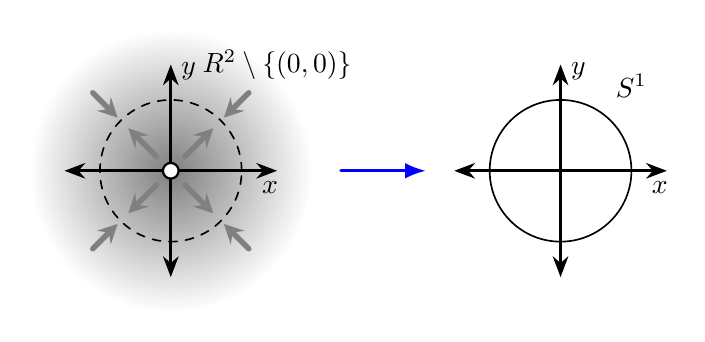
\begin{tikzpicture}[%
        scale=0.9,
        line width=1pt,
        line cap=round,
        >={Stealth[black]},
        every edge/.style={%
            draw=black,
            very thick
        },
        grayarrow/.style={%
            >=stealth,
            fill=gray,
            draw=gray,
            line width=0.7mm,
            ->
        }
    ]
        \filldraw[%
            even odd rule,
            inner color=gray,
            outer color=white,
            draw=white
        ]
            (0,0) circle (2);

        % Draw axes.
        \draw[<->] (-1.5,0) -- (1.5,0);
        \draw[<->] (0,-1.5) -- (0,1.5);
        \draw[<->] (4,0) -- (7,0);
        \draw[<->] (5.5,-1.5) -- (5.5,1.5);

        % Draw gray arrows indicating homotopy equivalence.
        \begin{scope}[every edge/.style=grayarrow]
            \draw(1.1,1.1) edge (0.75,0.75);
            \draw(-1.1,-1.1) edge (-0.75,-0.75);
            \draw(1.1,-1.1) edge (0.75,-0.75);
            \draw(-1.1,1.1) edge (-0.75,0.75);
            \draw(0.2,0.2) edge (0.6,0.6);
            \draw(-0.2,-0.2) edge (-0.6,-0.6);
            \draw(0.2,-0.2) edge (0.6,-0.6);
            \draw(-0.2,0.2) edge (-0.6,0.6);
        \end{scope}

        \draw[dashed,draw=black,semithick] (0,0) circle (1);
        \node[%
            fill=white,
            circle,
            thick,
            draw,
            inner sep=2pt,
            outer sep=3pt
        ]
            at (0,0) (O) {};
        \node at (1.4,0) [below] {$x$};
        \node at (0,1.4) [right] {$y$};
        \node at (1.5,1.5) {$\mathbb{R}^{2}\setminus\{(0,0)\}$};
        \draw[>=Latex,draw=blue,->] (2.4,0) -- (3.6,0);
        \draw[draw=black,semithick] (5.5,0) circle (1);
        \node at (6.9,0) [below] {$x$};
        \node at (5.5,1.4) [right] {$y$};
        \node at (6.5,1.2) {$S^{1}$};
    \end{tikzpicture}
\end{document}
                \caption{Homotopy Equivalence of
                         $\mathbb{R}^{2}\setminus\{(0,0)\}$ and $S^{1}$}
                \label{fig:homotopy_equivalence_between_the_plane_%
                       with_a_point_removed_and_the_unit_circle}
            \end{figure}
            \begin{ldefinition}{Disconnected Sets}{Disconnected_Sets}
                A disconnected subset of a topological space $X$ is a set
                $S\subseteq{X}$ such that there exist disjoint non-empty open
                sets $X_{1},X_{2}$ such that $S=X_{1}\cup{X_{2}}$.
            \end{ldefinition}
            \begin{ldefinition}{Connected Sets}{Connected_Sets}
                A connected subset of a topological space
                is a subset that is not disconnected.
            \end{ldefinition}
            \begin{ltheorem}{Homeomorphisms Preserve Connectedness}
                            {Homeomorphisms_Preserve_Connectedness}
                If $X$ and $Y$ are homeomorphic and
                $X$ is connected, then $Y$ is connected.
            \end{ltheorem}
            \begin{proof}
                Suppose not. If $Y$ is disconnected, then there are disjoint
                non-empty open sets $Y_{1},Y_{2}$ such that
                $Y=Y_{1}\cup{Y_{2}}$. But as $X$ and $Y$ are homeomorphic,
                there is a continuous bijection $f:X\rightarrow{Y}$. But then
                $f^{-1}(Y_{1})$ and $f^{-1}(Y_{2})$ are non-empty, as $f$ is a
                bijection, and moreoever they are disjoint open subsets of $X$,
                as $f$ is continuous. But then $X$ is disconnected,
                a contradiction. Thus, $Y$ is connected.
            \end{proof}
            \begin{theorem}
                There exists compact connected topological spaces of the same
                cardinality that are homotopy equivalent but not homeomorphic.
            \end{theorem}
            \begin{proof}
                Let $X=[-1,1]$, $Y=[-1,1]^{2}$ and define
                $f:X\rightarrow{Y}$ and $g:Y\rightarrow{X}$ by:
                \par
                \begin{minipage}[b]{0.49\textwidth}
                    \centering
                    \begin{equation}
                        f(x)=(x,0)
                    \end{equation}
                \end{minipage}
                \hfill
                \begin{minipage}[b]{0.49\textwidth}
                    \centering
                    \begin{equation}
                        g(x,y)=x
                    \end{equation}
                \end{minipage}
                \par\hfill\par
                Then $g\circ{f}=id_{X}$, and thus $g\circ{f}\simeq{id_{X}}$. But
                also $H(x,y,t)=(1-t)(x,0)+(x,y)$ is a homotopy between
                $f\circ{g}$ and $id_{Y}$, and thus $f\circ{g}\simeq{id_{Y}}$.
                Therefore $X$ and $Y$ are homotopy equivalent. Moreover, they
                are both compact, connected, and have the cardinality
                of the continuum. Suppose $h$ is a homeomorphism
                $h:X\rightarrow{Y}$ and let $h(0)=\mathbf{x}\in{Y}$. If $h$ is
                a homeomorphism between $X$ and $y$, then the restriction of $h$
                to $X\setminus\{0\}$ is a homeomophism between $[-1,0)\cup(0,1]$
                and $[-1,1]^{2}\setminus\{\mathbf{x}\}$. But
                $[-1,1]^{2}\setminus\{\mathbf{x}\}$ is connected, and
                $[-1,0)\cup(0,1]$ is not. But homeomorphisms preserve
                connectedness. Therefore, $X$ and $Y$ are not homeomorphic.
            \end{proof}
            We have seen that cardinality, connectedness, compactness, and
            homotopy equivalence are not enough to guarantee that two spaces are
            homeomorphic. However, thus far every example has included two
            spaces that are of different \textit{dimension}. Adding dimension to
            the list still does not guarantee that the two spaces will be
            homeomorphic. First, we show that $S^{2}\setminus\{(0,0,1)\}$ is
            homeomorphic to $D^{2}$.
            \begin{theorem}
                \label{thm:sphere_without_point_homeomorphic_to_plane}%
                $S^{2}\setminus\{(0,0,1)\}$ is homeomorphic to $\mathbb{R}^{2}$
            \end{theorem}
            \begin{proof}
                For let $f:S^{2}\setminus\{(0,0,1)\}\rightarrow \mathbb{R}^{2}$
                be the stereographic projection mapping:
                \begin{equation}
                    f(x,y,z)=\Big(\frac{x}{1-z},\frac{y}{1-z}\Big)
                \end{equation}
                If $(X,Y)\in\mathbb{R}^{2}$, let:
                \begin{align*}
                    x&=\frac{2X}{\norm{(X,Y)}^{2}+1}&
                    y&=\frac{2Y}{\norm{(X,Y)}^{2}+1}&
                    z&=\frac{\norm{(X,Y)}^{2}-1}{\norm{(X,Y)}^{2}+1} 
                \end{align*}
                Then:
                \begin{subequations}
                    \begin{align}
                        \Big(\frac{x}{1-z},\frac{y}{1-z}\Big)
                        &=\frac{\norm{(X,Y)}^{2}+1}{2}
                        \Big(\frac{2X}{\norm{(X,Y)}^{2}+ 1},
                             \frac{2Y}{\norm{(X,Y)}^{2}+1}\Big)\\
                        &=(X,Y)
                    \end{align}
                \end{subequations}
                and
                \begin{subequations}
                    \begin{align}
                        \norm{(x,y,z)}&=\sqrt{%
                            \frac{4\norm{(X,Y)}^{2}+\norm{(X,Y)}^{4}-
                                  2\norm{(X,Y)}^{2}+1}{(\norm{(X,Y)}+1)^{2}}%
                        }\\
                        &=\sqrt{\frac{\norm{(X,Y)}^{4}+2\norm{(X,Y)}^{2}+1}
                                     {(\norm{(X,Y)}^{2}+1)^{2}}}\\
                        &=\sqrt{%
                            \frac{(\norm{(X,Y)}^{2}+1)^{2}}
                                 {(\norm{(X,Y)}^{2}+1)^{2}}%
                        }
                    \end{align}
                \end{subequations}
                Which evaluates to one. Thus,
                $(x,y,z)\in S^{2}\setminus\{(0,0,1)\}$, and $f$ is surjective.
                If $f(x_{1},y_{1},z_{1})=f(x_{2},y_{2},z_{2})$, then
                $z_{1}=z_{2}$. For since
                $(x_{1},y_{1},z_{1})\in S^{2}\setminus\{(0,0,1)\}$,
                and therefore $x_{1}^{2}+y_{1}^{2}=1-z_{1}^{2}$, we have:
                \begin{equation}
                    \norm{(X,Y)}^{2}
                    =\frac{x_{1}^2+y_{1}^2}{(1-z_{1})^{2}}
                    =\frac{1-z_{1}^{2}}{(1-z_{1})^{2}}
                    =\frac{x_{2}^{2}+y_{2}^{2}}{(1-z_{2})^{2}}
                    =\frac{1-z_{2}^{2}}{(1-z_{2})^{2}}
                \end{equation}
                So we have:
                \begin{equation}
                    \frac{1-z_{1}^{2}}{(1-z_{1})^{2}}
                    =\frac{1-z_{2}^{2}}{(1-z_{2})^{2}}
                    \Rightarrow
                    \frac{1+z_{1}}{1-z_{1}}
                    =\frac{1+z_{2}}{1-z_{2}}
                \end{equation}
                But the function $g(x)=\frac{1+x}{1-x}$ is an injective function
                and therefore $z_{1}=z_{2}$. From this $x_{1}=x_{2}$ and
                $y_{1}=y_{2}$. Thus, $f$ is a bijection. Moreoever,
                $f$ is continuous and:
                \begin{equation}
                    f^{-1}(X,Y)
                    =\Big(\frac{2X}{\norm{(X,Y)}^{2}+1},
                        \frac{2Y}{\norm{(X,Y)}^{2}+1},
                        \frac{\norm{(X,Y)}^{2}-1}{\norm{(X,Y)}^{2}+1}\Big)
                \end{equation}
                which is continuous. $f$ is a homeomorphism.
            \end{proof}
            Fig.~\ref{fig:stereographic_projection} depicts the stereographic
            projection used to prove
            Thm.~\ref{thm:sphere_without_point_homeomorphic_to_plane}.
            It can be seen that $(0,0,1)$ projects `to infinity'. Because of
            this, it is not uncommon to call this point infinity. Next, we
            prove that $\mathbb{R}^{2}$ is homeomorphic to $D^{2}$, almost
            completing our claim that $S^{2}\setminus\{(0,0,1)\}$
            is homeomorphic to $D^{2}$.
            \begin{figure}[H]
                \captionsetup{type=figure}
                \centering
                \documentclass[crop,class=article]{standalone}
%----------------------------Preamble-------------------------------%
%---------------------------Packages----------------------------%
\usepackage{geometry}
\geometry{b5paper, margin=1.0in}
\usepackage[T1]{fontenc}
\usepackage{graphicx, float}            % Graphics/Images.
\usepackage{natbib}                     % For bibliographies.
\bibliographystyle{agsm}                % Bibliography style.
\usepackage[french, english]{babel}     % Language typesetting.
\usepackage[dvipsnames]{xcolor}         % Color names.
\usepackage{listings}                   % Verbatim-Like Tools.
\usepackage{mathtools, esint, mathrsfs} % amsmath and integrals.
\usepackage{amsthm, amsfonts, amssymb}  % Fonts and theorems.
\usepackage{tcolorbox}                  % Frames around theorems.
\usepackage{upgreek}                    % Non-Italic Greek.
\usepackage{fmtcount, etoolbox}         % For the \book{} command.
\usepackage[newparttoc]{titlesec}       % Formatting chapter, etc.
\usepackage{titletoc}                   % Allows \book in toc.
\usepackage[nottoc]{tocbibind}          % Bibliography in toc.
\usepackage[titles]{tocloft}            % ToC formatting.
\usepackage{pgfplots, tikz}             % Drawing/graphing tools.
\usepackage{imakeidx}                   % Used for index.
\usetikzlibrary{
    calc,                   % Calculating right angles and more.
    angles,                 % Drawing angles within triangles.
    arrows.meta,            % Latex and Stealth arrows.
    quotes,                 % Adding labels to angles.
    positioning,            % Relative positioning of nodes.
    decorations.markings,   % Adding arrows in the middle of a line.
    patterns,
    arrows
}                                       % Libraries for tikz.
\pgfplotsset{compat=1.9}                % Version of pgfplots.
\usepackage[font=scriptsize,
            labelformat=simple,
            labelsep=colon]{subcaption} % Subfigure captions.
\usepackage[font={scriptsize},
            hypcap=true,
            labelsep=colon]{caption}    % Figure captions.
\usepackage[pdftex,
            pdfauthor={Ryan Maguire},
            pdftitle={Mathematics and Physics},
            pdfsubject={Mathematics, Physics, Science},
            pdfkeywords={Mathematics, Physics, Computer Science, Biology},
            pdfproducer={LaTeX},
            pdfcreator={pdflatex}]{hyperref}
\hypersetup{
    colorlinks=true,
    linkcolor=blue,
    filecolor=magenta,
    urlcolor=Cerulean,
    citecolor=SkyBlue
}                           % Colors for hyperref.
\usepackage[toc,acronym,nogroupskip,nopostdot]{glossaries}
\usepackage{glossary-mcols}
%------------------------Theorem Styles-------------------------%
\theoremstyle{plain}
\newtheorem{theorem}{Theorem}[section]

% Define theorem style for default spacing and normal font.
\newtheoremstyle{normal}
    {\topsep}               % Amount of space above the theorem.
    {\topsep}               % Amount of space below the theorem.
    {}                      % Font used for body of theorem.
    {}                      % Measure of space to indent.
    {\bfseries}             % Font of the header of the theorem.
    {}                      % Punctuation between head and body.
    {.5em}                  % Space after theorem head.
    {}

% Italic header environment.
\newtheoremstyle{thmit}{\topsep}{\topsep}{}{}{\itshape}{}{0.5em}{}

% Define environments with italic headers.
\theoremstyle{thmit}
\newtheorem*{solution}{Solution}

% Define default environments.
\theoremstyle{normal}
\newtheorem{example}{Example}[section]
\newtheorem{definition}{Definition}[section]
\newtheorem{problem}{Problem}[section]

% Define framed environment.
\tcbuselibrary{most}
\newtcbtheorem[use counter*=theorem]{ftheorem}{Theorem}{%
    before=\par\vspace{2ex},
    boxsep=0.5\topsep,
    after=\par\vspace{2ex},
    colback=green!5,
    colframe=green!35!black,
    fonttitle=\bfseries\upshape%
}{thm}

\newtcbtheorem[auto counter, number within=section]{faxiom}{Axiom}{%
    before=\par\vspace{2ex},
    boxsep=0.5\topsep,
    after=\par\vspace{2ex},
    colback=Apricot!5,
    colframe=Apricot!35!black,
    fonttitle=\bfseries\upshape%
}{ax}

\newtcbtheorem[use counter*=definition]{fdefinition}{Definition}{%
    before=\par\vspace{2ex},
    boxsep=0.5\topsep,
    after=\par\vspace{2ex},
    colback=blue!5!white,
    colframe=blue!75!black,
    fonttitle=\bfseries\upshape%
}{def}

\newtcbtheorem[use counter*=example]{fexample}{Example}{%
    before=\par\vspace{2ex},
    boxsep=0.5\topsep,
    after=\par\vspace{2ex},
    colback=red!5!white,
    colframe=red!75!black,
    fonttitle=\bfseries\upshape%
}{ex}

\newtcbtheorem[auto counter, number within=section]{fnotation}{Notation}{%
    before=\par\vspace{2ex},
    boxsep=0.5\topsep,
    after=\par\vspace{2ex},
    colback=SeaGreen!5!white,
    colframe=SeaGreen!75!black,
    fonttitle=\bfseries\upshape%
}{not}

\newtcbtheorem[use counter*=remark]{fremark}{Remark}{%
    fonttitle=\bfseries\upshape,
    colback=Goldenrod!5!white,
    colframe=Goldenrod!75!black}{ex}

\newenvironment{bproof}{\textit{Proof.}}{\hfill$\square$}
\tcolorboxenvironment{bproof}{%
    blanker,
    breakable,
    left=3mm,
    before skip=5pt,
    after skip=10pt,
    borderline west={0.6mm}{0pt}{green!80!black}
}

\AtEndEnvironment{lexample}{$\hfill\textcolor{red}{\blacksquare}$}
\newtcbtheorem[use counter*=example]{lexample}{Example}{%
    empty,
    title={Example~\theexample},
    boxed title style={%
        empty,
        size=minimal,
        toprule=2pt,
        top=0.5\topsep,
    },
    coltitle=red,
    fonttitle=\bfseries,
    parbox=false,
    boxsep=0pt,
    before=\par\vspace{2ex},
    left=0pt,
    right=0pt,
    top=3ex,
    bottom=1ex,
    before=\par\vspace{2ex},
    after=\par\vspace{2ex},
    breakable,
    pad at break*=0mm,
    vfill before first,
    overlay unbroken={%
        \draw[red, line width=2pt]
            ([yshift=-1.2ex]title.south-|frame.west) to
            ([yshift=-1.2ex]title.south-|frame.east);
        },
    overlay first={%
        \draw[red, line width=2pt]
            ([yshift=-1.2ex]title.south-|frame.west) to
            ([yshift=-1.2ex]title.south-|frame.east);
    },
}{ex}

\AtEndEnvironment{ldefinition}{$\hfill\textcolor{Blue}{\blacksquare}$}
\newtcbtheorem[use counter*=definition]{ldefinition}{Definition}{%
    empty,
    title={Definition~\thedefinition:~{#1}},
    boxed title style={%
        empty,
        size=minimal,
        toprule=2pt,
        top=0.5\topsep,
    },
    coltitle=Blue,
    fonttitle=\bfseries,
    parbox=false,
    boxsep=0pt,
    before=\par\vspace{2ex},
    left=0pt,
    right=0pt,
    top=3ex,
    bottom=0pt,
    before=\par\vspace{2ex},
    after=\par\vspace{1ex},
    breakable,
    pad at break*=0mm,
    vfill before first,
    overlay unbroken={%
        \draw[Blue, line width=2pt]
            ([yshift=-1.2ex]title.south-|frame.west) to
            ([yshift=-1.2ex]title.south-|frame.east);
        },
    overlay first={%
        \draw[Blue, line width=2pt]
            ([yshift=-1.2ex]title.south-|frame.west) to
            ([yshift=-1.2ex]title.south-|frame.east);
    },
}{def}

\AtEndEnvironment{ltheorem}{$\hfill\textcolor{Green}{\blacksquare}$}
\newtcbtheorem[use counter*=theorem]{ltheorem}{Theorem}{%
    empty,
    title={Theorem~\thetheorem:~{#1}},
    boxed title style={%
        empty,
        size=minimal,
        toprule=2pt,
        top=0.5\topsep,
    },
    coltitle=Green,
    fonttitle=\bfseries,
    parbox=false,
    boxsep=0pt,
    before=\par\vspace{2ex},
    left=0pt,
    right=0pt,
    top=3ex,
    bottom=-1.5ex,
    breakable,
    pad at break*=0mm,
    vfill before first,
    overlay unbroken={%
        \draw[Green, line width=2pt]
            ([yshift=-1.2ex]title.south-|frame.west) to
            ([yshift=-1.2ex]title.south-|frame.east);},
    overlay first={%
        \draw[Green, line width=2pt]
            ([yshift=-1.2ex]title.south-|frame.west) to
            ([yshift=-1.2ex]title.south-|frame.east);
    }
}{thm}

%--------------------Declared Math Operators--------------------%
\DeclareMathOperator{\adjoint}{adj}         % Adjoint.
\DeclareMathOperator{\Card}{Card}           % Cardinality.
\DeclareMathOperator{\curl}{curl}           % Curl.
\DeclareMathOperator{\diam}{diam}           % Diameter.
\DeclareMathOperator{\dist}{dist}           % Distance.
\DeclareMathOperator{\Div}{div}             % Divergence.
\DeclareMathOperator{\Erf}{Erf}             % Error Function.
\DeclareMathOperator{\Erfc}{Erfc}           % Complementary Error Function.
\DeclareMathOperator{\Ext}{Ext}             % Exterior.
\DeclareMathOperator{\GCD}{GCD}             % Greatest common denominator.
\DeclareMathOperator{\grad}{grad}           % Gradient
\DeclareMathOperator{\Ima}{Im}              % Image.
\DeclareMathOperator{\Int}{Int}             % Interior.
\DeclareMathOperator{\LC}{LC}               % Leading coefficient.
\DeclareMathOperator{\LCM}{LCM}             % Least common multiple.
\DeclareMathOperator{\LM}{LM}               % Leading monomial.
\DeclareMathOperator{\LT}{LT}               % Leading term.
\DeclareMathOperator{\Mod}{mod}             % Modulus.
\DeclareMathOperator{\Mon}{Mon}             % Monomial.
\DeclareMathOperator{\multideg}{mutlideg}   % Multi-Degree (Graphs).
\DeclareMathOperator{\nul}{nul}             % Null space of operator.
\DeclareMathOperator{\Ord}{Ord}             % Ordinal of ordered set.
\DeclareMathOperator{\Prin}{Prin}           % Principal value.
\DeclareMathOperator{\proj}{proj}           % Projection.
\DeclareMathOperator{\Refl}{Refl}           % Reflection operator.
\DeclareMathOperator{\rk}{rk}               % Rank of operator.
\DeclareMathOperator{\sgn}{sgn}             % Sign of a number.
\DeclareMathOperator{\sinc}{sinc}           % Sinc function.
\DeclareMathOperator{\Span}{Span}           % Span of a set.
\DeclareMathOperator{\Spec}{Spec}           % Spectrum.
\DeclareMathOperator{\supp}{supp}           % Support
\DeclareMathOperator{\Tr}{Tr}               % Trace of matrix.
%--------------------Declared Math Symbols--------------------%
\DeclareMathSymbol{\minus}{\mathbin}{AMSa}{"39} % Unary minus sign.
%------------------------New Commands---------------------------%
\DeclarePairedDelimiter\norm{\lVert}{\rVert}
\DeclarePairedDelimiter\ceil{\lceil}{\rceil}
\DeclarePairedDelimiter\floor{\lfloor}{\rfloor}
\newcommand*\diff{\mathop{}\!\mathrm{d}}
\newcommand*\Diff[1]{\mathop{}\!\mathrm{d^#1}}
\renewcommand*{\glstextformat}[1]{\textcolor{RoyalBlue}{#1}}
\renewcommand{\glsnamefont}[1]{\textbf{#1}}
\renewcommand\labelitemii{$\circ$}
\renewcommand\thesubfigure{%
    \arabic{chapter}.\arabic{figure}.\arabic{subfigure}}
\addto\captionsenglish{\renewcommand{\figurename}{Fig.}}
\numberwithin{equation}{section}

\renewcommand{\vector}[1]{\boldsymbol{\mathrm{#1}}}

\newcommand{\uvector}[1]{\boldsymbol{\hat{\mathrm{#1}}}}
\newcommand{\topspace}[2][]{(#2,\tau_{#1})}
\newcommand{\measurespace}[2][]{(#2,\varSigma_{#1},\mu_{#1})}
\newcommand{\measurablespace}[2][]{(#2,\varSigma_{#1})}
\newcommand{\manifold}[2][]{(#2,\tau_{#1},\mathcal{A}_{#1})}
\newcommand{\tanspace}[2]{T_{#1}{#2}}
\newcommand{\cotanspace}[2]{T_{#1}^{*}{#2}}
\newcommand{\Ckspace}[3][\mathbb{R}]{C^{#2}(#3,#1)}
\newcommand{\funcspace}[2][\mathbb{R}]{\mathcal{F}(#2,#1)}
\newcommand{\smoothvecf}[1]{\mathfrak{X}(#1)}
\newcommand{\smoothonef}[1]{\mathfrak{X}^{*}(#1)}
\newcommand{\bracket}[2]{[#1,#2]}

%------------------------Book Command---------------------------%
\makeatletter
\renewcommand\@pnumwidth{1cm}
\newcounter{book}
\renewcommand\thebook{\@Roman\c@book}
\newcommand\book{%
    \if@openright
        \cleardoublepage
    \else
        \clearpage
    \fi
    \thispagestyle{plain}%
    \if@twocolumn
        \onecolumn
        \@tempswatrue
    \else
        \@tempswafalse
    \fi
    \null\vfil
    \secdef\@book\@sbook
}
\def\@book[#1]#2{%
    \refstepcounter{book}
    \addcontentsline{toc}{book}{\bookname\ \thebook:\hspace{1em}#1}
    \markboth{}{}
    {\centering
     \interlinepenalty\@M
     \normalfont
     \huge\bfseries\bookname\nobreakspace\thebook
     \par
     \vskip 20\p@
     \Huge\bfseries#2\par}%
    \@endbook}
\def\@sbook#1{%
    {\centering
     \interlinepenalty \@M
     \normalfont
     \Huge\bfseries#1\par}%
    \@endbook}
\def\@endbook{
    \vfil\newpage
        \if@twoside
            \if@openright
                \null
                \thispagestyle{empty}%
                \newpage
            \fi
        \fi
        \if@tempswa
            \twocolumn
        \fi
}
\newcommand*\l@book[2]{%
    \ifnum\c@tocdepth >-3\relax
        \addpenalty{-\@highpenalty}%
        \addvspace{2.25em\@plus\p@}%
        \setlength\@tempdima{3em}%
        \begingroup
            \parindent\z@\rightskip\@pnumwidth
            \parfillskip -\@pnumwidth
            {
                \leavevmode
                \Large\bfseries#1\hfill\hb@xt@\@pnumwidth{\hss#2}
            }
            \par
            \nobreak
            \global\@nobreaktrue
            \everypar{\global\@nobreakfalse\everypar{}}%
        \endgroup
    \fi}
\newcommand\bookname{Book}
\renewcommand{\thebook}{\texorpdfstring{\Numberstring{book}}{book}}
\providecommand*{\toclevel@book}{-2}
\makeatother
\titleformat{\part}[display]
    {\Large\bfseries}
    {\partname\nobreakspace\thepart}
    {0mm}
    {\Huge\bfseries}
\titlecontents{part}[0pt]
    {\large\bfseries}
    {\partname\ \thecontentslabel: \quad}
    {}
    {\hfill\contentspage}
\titlecontents{chapter}[0pt]
    {\bfseries}
    {\chaptername\ \thecontentslabel:\quad}
    {}
    {\hfill\contentspage}
\newglossarystyle{longpara}{%
    \setglossarystyle{long}%
    \renewenvironment{theglossary}{%
        \begin{longtable}[l]{{p{0.25\hsize}p{0.65\hsize}}}
    }{\end{longtable}}%
    \renewcommand{\glossentry}[2]{%
        \glstarget{##1}{\glossentryname{##1}}%
        &\glossentrydesc{##1}{~##2.}
        \tabularnewline%
        \tabularnewline
    }%
}
\newglossary[not-glg]{notation}{not-gls}{not-glo}{Notation}
\newcommand*{\newnotation}[4][]{%
    \newglossaryentry{#2}{type=notation, name={\textbf{#3}, },
                          text={#4}, description={#4},#1}%
}
%--------------------------LENGTHS------------------------------%
% Spacings for the Table of Contents.
\addtolength{\cftsecnumwidth}{1ex}
\addtolength{\cftsubsecindent}{1ex}
\addtolength{\cftsubsecnumwidth}{1ex}
\addtolength{\cftfignumwidth}{1ex}
\addtolength{\cfttabnumwidth}{1ex}

% Indent and paragraph spacing.
\setlength{\parindent}{0em}
\setlength{\parskip}{0em}
%--------------------------Main Document----------------------------%
\begin{document}
    \begin{tikzpicture}[scale=5, >=triangle 45]
        % Draw the main coordinate system axes
        \draw[thick,->] (0,0,0)--(1.7,0,0) node[right] {$y$};
        \draw[thick,->] (0,0,0)--(0,1.3,0) node[above]{$z$};
        \draw[thick,->] (0,0,0)--(0,0,1.7) node[below left]{$x$};

        % The point (x,y,z)
        \coordinate (A) at (0.577350269,0.577350269,0.577350269);

        % The projection point (X,Y)
        \node[circle, inner sep=0pt, outer sep=1mm]
            (B) at (1.3660254,0,1.3660254) {};

        % Draw blue line "inside" sphere.
        \draw[draw=blue,semithick] (0,1,0) -- (A);

        % Draw sphere.
        \shade[ball color=gray, opacity=0.6]
            (1cm,0) arc (0:-180:1cm and 5mm)
            arc (180:0:1cm and 1cm);
        
        % Draw blue line "outside" of sphere.
        \draw[draw=blue, semithick, >=stealth, ->] (A)--(B);

        % Draw projection lines.
        \begin{scope}[every path/.style={dashed,thin}]
            \path (0,0,0) edge (1.3660254,0,1.3660254);
            \path (0,0,1.3660254) edge (1.3660254,0,1.3660254);
            \path (1.3660254,0,0) edge (1.3660254,0,1.3660254);
            \path (0,0,0.5774) edge (0.5774,0,0.5774);
            \path (0.5774,0,0) edge (0.5774,0,0.5774);
            \path (0.5774,0,0.5774) edge (0.5774,0.5774,0.5774);
            \path (0,0,0.5774) edge (0.5774,0,0.5774);
        \end{scope}

        % Draw the position vector.
        \draw[dashed,semithick] (0,0,0) -- (0.5774,0.5774,0.5774);

        \filldraw[black] (0.57735,0.57735,0.57735) circle (0.15mm);
        \filldraw[red] (1.3660254,0,1.3660254) circle (0.15mm);
        \node at (A) [above right] {$(x,y,z)$};
        \node at (B) [below right] {$(X,Y)$};
    \end{tikzpicture}
\end{document}
                \caption{Stereographic Projection of the Sphere onto the Plane.}
                \label{fig:stereographic_projection}
            \end{figure}
            \begin{theorem}
                $\mathbb{R}^{2}$ is homeomorphic to $D^{2}$.
            \end{theorem}
            \begin{proof}
                Let $f:D^{2}\rightarrow\mathbb{R}^{2}$
                be defined by:
                \begin{equation}
                    f(\mathbf{x})=\frac{\mathbf{x}}{1-\norm{\mathbf{x}}}
                \end{equation}
                $f$ is surjective. For $\mathbf{0}\mapsto\mathbf{0}$ and if
                $\mathbf{y}\in\mathbb{R}^2\setminus\{\mathbf{0}\}$, then let
                $\mathbf{x}=\frac{\mathbf{y}}{1+\norm{\mathbf{y}}}$. Then:
                \begin{equation}
                    \norm{\mathbf{x}}
                    =\frac{\norm{\mathbf{y}}}{1+\norm{\mathbf{y}}}<1
                \end{equation}
                and thus $\mathbf{x}\in D^{2}$. But:
                \begin{equation}
                    f(\mathbf{x})
                    =\frac{\mathbf{y}}{1+\norm{\mathbf{y}}}
                    \Big(
                        1-\frac{\norm{\mathbf{y}}}{1+\norm{\mathbf{y}}}
                    \Big)^{-1}
                    =\mathbf{y}
                \end{equation}
                Moreover, $f$ is injective.
                For if
                $f(\mathbf{x}_{1})=f(\mathbf{x}_{2})$,
                then:
                \begin{equation}
                    \frac{\norm{\mathbf{x}_{1}}}{1+\norm{\mathbf{x}_{1}}}
                    =\norm{f(\mathbf{x}_{1})}
                    =\norm{f(\mathbf{x}_{2})}
                    =\frac{\norm{\mathbf{x}_{2}}}{1+\norm{\mathbf{x}}_{2}}
                \end{equation}
                and therefore
                $\norm{\mathbf{x}}_{1}=\norm{\mathbf{x}_{2}}$.
                But from the definition of $f$:
                \begin{equation}
                    \frac{\mathbf{x}_{1}}{1+\norm{\mathbf{x}_{1}}}
                    =\frac{\mathbf{x}_{2}}{1+\norm{\mathbf{x}_{2}}}
                \end{equation}
                and therefore $\mathbf{x}_{1}=\mathbf{x}_{2}$.
                $f$ is bijective.
                Moreover, $f$ is continuous. Finally,
                \begin{equation}
                    f^{-1}(\mathbf{y})
                    =\frac{\mathbf{y}}{1+\norm{\mathbf{y}}}                    
                \end{equation}
                which is continuous. $f$ is a homeomorphism.
            \end{proof}
            \begin{theorem}
                $S^{2}\setminus\{(0,0,1)\}$ is homeomorphic to $D^{2}$.
            \end{theorem}
            \begin{proof}
                For $S^{2}\setminus\{(0,0,1)\}$ is homeomorphic to
                $\mathbb{R}^{2}$, and $\mathbb{R}^{2}$ is homeomorphic to
                $D^{2}$. But homeomorphism is an equivalence relation, and
                thus $S^{2}\setminus\{(0,0,1)\}$ is homeomorphic to $D^{2}$.
            \end{proof}
            \begin{figure}[H]
                \centering
                \captionsetup{type=figure}
                \includegraphics{images/Sphere_to_Disk_Homeo.pdf}
                \caption{Homeomorphism of a Sphere w/o a Point to an Open Disk}
                \label{fig:homeomorphism_S_2_wo_North_Pole_and_R_2_2}
            \end{figure}
            We can use the fact that $S^{2}\setminus \{(0,0,1)\}$ is
            homeomorphic to $D^{2}$ to construct examples of topological
            manifolds of the same dimensions that are homotopy equivalent, but
            not homeomorphic. We may generalize to $S^{2}$ with $n$ points
            removed is homeomorphic to $D^{2}$ with $n-1$ points removed.
            We now define the notion of \textit{manifold} and
            \textit{dimension}.
            \begin{ldefinition}{Topological Manifold}{Topological_Manifold}
                An $n$ dimensional manifold is a Second-Countable Hausdorff
                topological space $X$ such that for all $p\in{X}$ there is an
                open neighborhood $\mathcal{U}$ of $p$, such that $\mathcal{U}$
                is homeomorphic to $\mathbb{R}^{n}$.
            \end{ldefinition}
            It can be shown that if $X$ and $Y$ are homeomorphic manifolds,
            then they are of the same dimension. This is simply because
            $\mathbb{R}^{n}$ is homeomorphic to $\mathbb{R}^{m}$ if and only if
            $n=m$. Therefore, homeomorphisms preserve dimension. We use the
            fact that a sphere is not homeomorphic to a torus. This can be
            proved by considering the \textit{fundamental group} of the sphere
            and the torus, but can also be shown in a more elementary way if
            we're allowed to assume the Jordan Curve Theorem.
            \begin{ldefinition}{Jordan Curve}{Jordan_Curve}
                A Jordan Curve is a continuous injective function
                $f:S^{1}\rightarrow\mathbb{R}^{2}$.
            \end{ldefinition}
            With this we now state, but do not prove, the Jordan Curve Theorem.
            \begin{ftheorem}{Jordan Curve Theorem}{Jordan_Curve_Theorem}
                If $\Gamma$ is a Jordan Curve, then there exists two unique
                disjoint open connected sets $\interior[](\Gamma)$ and $\exterior[](\Gamma)$,
                called the interior and exterior of $\Gamma$, such that:
                \begin{equation}
                    \mathbb{R}^{2}\setminus\Gamma=\interior[](\Gamma)\cup\exterior[](\Gamma)
                \end{equation}
                And such that $\partial\interior[](\Gamma)=\Gamma$ and
                $\partial\exterior[](\Gamma)=\Gamma$. $\interior[](\Gamma)$ is
                bounded and $\exterior[](\Gamma)$ is unbounded.
            \end{ftheorem}
            The Jordan Curve Theorem implies that the injective continuous
            image of $S^{1}$ into the sphere $S^{2}$ will cut the
            sphere into two parts. That is, given a circle and
            a continuous one-to-one mapping into the sphere, the
            result bisects the sphere into two parts.
            \begin{theorem}
                \label{thm:Sphere_Without_Circle_Is_Disconnected}
                If $f:S^{1}\rightarrow{S}^{2}$ is a continuous injective
                function, then there exists two disjoint open connected
                sets $\mathcal{U}_{1}$ and $\mathcal{U}_{2}$ such that:
                \begin{equation}
                    S^{2}\setminus{f}(S^{1})
                    =\mathcal{U}_{1}\cup\mathcal{U}_{2}
                \end{equation}
            \end{theorem}
            \begin{proof}
                First note that $f$ is not surjective. For if it were,
                remove two points from $S^{1}$ and remove the corresponding
                points from $S^{2}$. Then the restriction of $f$ to the
                remaining set is still bijective and continuous. But
                $S^{2}$ without two points is connected, whereas $S^{1}$
                without two points is disconnected. Therefore $f$ is not
                surjective. But then there is a point $\mathbf{y}\in{S}^{2}$
                such that, for all $x\in{S}^{1}$, $f(x)\ne\mathbb{R}$.
                But then $f:S^{1}\rightarrow{S}^{2}\setminus\mathbf{y}$
                is still a continuous injective function. But
                $S^{2}\setminus\mathbf{y}$ is homeomorphic to $\mathbb{R}^{2}$.
                Thus there is a
                $g:S^{2}\setminus\{\mathbf{y}\}\rightarrow\mathbb{R}$
                such that $g$ is a homeomorphism. But then $\Gamma=g\circ{f}$
                is a Jordan Curve. By the Jordan Curve Theorem there are two
                disjoint open connected sets $\interior[](\Gamma)$ and $\exterior[](\Gamma)$
                such that
                $\interior[](\Gamma)\cup\exterior[](\Gamma)=\mathbb{R}^{2}\setminus\Gamma$.
                Define the following:
                \par
                \begin{subequations}
                    \begin{minipage}[b]{0.49\textwidth}
                        \centering
                        \begin{equation}
                            \mathcal{U}_{1}=g^{-1}\big(\interior[](\Gamma)\big)
                        \end{equation}
                    \end{minipage}
                    \hfill
                    \begin{minipage}[b]{0.49\textwidth}
                        \begin{equation}
                            \mathcal{U}_{2}
                            =g^{-1}\big(\exterior[](\Gamma)\big)\cup\{\mathbf{y}\}
                        \end{equation}
                    \end{minipage}
                \end{subequations}
                \par\hfill\par
                Then $\mathcal{U}_{1}$ and $\mathcal{U}_{2}$ are open, disjoint,
                connected, and cover $S^{2}\setminus{f}(S^{1})$.
            \end{proof}
            With this we can prove that $S^{2}$ and $T^{1}$, the sphere and the
            torus, are not homeomorphic.
            \begin{ltheorem}{$S^{1}$ is not Homeomorphic to $T^{1}$}
                            {Circle_Not_Homeo_to_Torus}
                There is no homeomorphism between the sphere $S^{2}$ and
                the torus $T^{1}$.
            \end{ltheorem}
            \begin{proof}
                The Torus is the Cartesian product of two circles,
                $T^{1}=S^{1}\times{S}^{1}$, and by removing the inner circle we
                are left with a connected set. Suppose the two are homeomorphic
                and let $f:T^{1}\rightarrow{S}^{2}$ be a homeomorphism. Then the
                restriction of $f$ to $T^{1}\setminus{S}^{1}$ is a homeomorphism
                with $S^{2}\setminus{f}(S^{1})$. But by
                Thm.~\ref{thm:Sphere_Without_Circle_Is_Disconnected}
                $S^{2}\setminus{f}(S^{1})$ is disconnected, a contradiction.
                Therefore there is no homeomorphism.
            \end{proof}
            Finally, we'll use the following visual representation of a torus:
            \begin{figure}[H]
                \centering
                \captionsetup{type=figure}
                \resizebox{\textwidth}{!}{%
                    \includegraphics{images/Square_to_Torus.pdf}
                }
                \caption{Turning a Square into a Torus}
                \label{fig:plane_representation_of_a_torus}
            \end{figure}
            It should be intuitively clear that both the torus and the sphere
            are two dimensional topological manifolds. If we remove a finite
            number of points from either of these we are still left with
            two dimensional manifolds.
            \begin{theorem}
                There exist manifolds $X$ and $Y$ such that
                $\dim(X)=\dim(Y)$, ${X}\simeq{Y}$,
                yet $X$ and $Y$ are not homeomorphic.
            \end{theorem}
            \begin{proof}
                For let $X=S^{2}\setminus\{(0,0,1),(0,1,0),(1,0,0)\}$, and let
                $Y=T^{2}\setminus\{(1,0,0)\}$. That is, $X$ is a sphere with
                three points removed, and $Y$ is a torus with one point removed.
                Then $\dim(X)=\dim(Y)=2$. Moreover, $X\simeq Y$. For $X$ is
                homeomorphic to the plane with $2$ points removed. This is
                homotopy equivalent to a figure $8$. Using the square
                representation of a torus in
                Fig.~\ref{fig:plane_representation_of_a_torus} we see that the
                torus with a point removed is also homotopy equivalent to a
                figure $8$. But homotopy equivalence is an equivalence relation,
                and thus $X\simeq Y$. But the a sphere is not homeomorphic to a
                torus, and similarly a sphere with $3$ points removed is not
                homeomorphic to a torus with $1$ point removed.
            \end{proof}
            \begin{figure}[H]
                    \centering
                    \captionsetup{type=figure}
                    \resizebox{\textwidth}{!}{%
                        \begin{tikzpicture}[%
    every edge/.style={draw=black},
    scale=1.7,
    >=latex
]
    \draw[ball color=gray!40, opacity=0.4] (0,0) circle (1cm);
    \draw (-1,0) arc (180:360:1 and 0.3);
    \draw[dashed] (1,0) arc (0:180:1 and 0.3);
    \draw[fill=white] (0.55,0.55) circle (0.75pt);
    \draw[fill=white] (0.65,0.65) circle (0.75pt);
    \draw[fill=white] (0.5,0.72)  circle (0.75pt);
    \draw[->] (1.3,0) to (2.3,0);
    \draw[fill=gray, shading angle=215]
        (2.5,-0.5)--(3.2,0.5)--(5.5,0.5)--(4.8,-0.5)--cycle;
    \draw[densely dashed] (3.7,0) circle (0.295);
    \draw[densely dashed] (4.3,0) circle (0.295);
    \draw[fill=white] (3.7,0) circle (0.75pt);
    \draw[fill=white] (4.3,0) circle (0.75pt);
    \draw[->] (5.7,0) to [in=90,out=0] (7,-1);
    \draw[->] (1.2,-2.3)--(2,-2.3);
    \draw[%
        postaction={decorate},
        decoration={%
            markings,
            mark=at position .145 with \arrow{latex},
            mark=at position .375 with \arrow{latex},
            mark=at position .395 with \arrow{latex},
            mark=at position .615 with \arrowreversed{latex},
            mark=at position .855 with \arrowreversed{latex},
            mark=at position .875 with \arrowreversed{latex}
        },
        fill=gray,
        shading angle=215
    ] (-0.75,-3)--(0.75,-3)--(0.75,-1.5)--(-0.75,-1.5)--cycle;
    \draw[fill=white] (0,-2.3) circle (0.75pt);
    \draw[%
        postaction={decorate},
        decoration={%
            markings,
            mark=at position .5 with \arrow{latex},
            mark=at position .55 with \arrow{latex}
        }
    ]   (3.1,-2.3) arc[%
                start angle=0,
                delta angle=-360,
                x radius=.35,
                y radius=.75
        ];
    \draw (2.75,-1.55) -- (4.75,-1.55);
    \draw[%
        postaction={decorate},
        decoration={%
        markings,
        mark=at position .5 with \arrow{latex},
        mark=at position .55 with \arrow{latex}
        }
    ]   (5.1cm,-2.3cm) arc[%
            start angle=0,
            delta angle=-360,
            x radius=.35,
            y radius=.75
        ];
    \draw[->] (5.4,-2.3)--(6.3,-2.3);
    \draw (7,-1.8) circle (0.5);
    \draw (7,-2.8) circle (0.5);
\end{tikzpicture}%
                    }
                    \caption{Equivalency of $S^{2}\setminus\{a,b,c\}$,
                             $T^{2}\setminus\{\alpha\}$, and a figure-8.}
                    \label{fig:homotopy_equivalence_sphere_%
                           with_3_holes_torus_with_1_hole}
            \end{figure} 
            Fig.~\ref{fig:homotopy_equivalence_sphere_%
                           with_3_holes_torus_with_1_hole} shows how both
            $S^{2}$ with three points removed and $T^{2}$ with one point removed
            are homotopy equivalent. Recall that
            $\mathbb{R}^{2}\setminus \{(0,0)\}$ is homotopy equivalent to
            $S^{1}$. In a similar manner, the plane with two points removed is
            homotopy equivalent to two circles whose intersection contains a
            single points (That is, a figure-$8$). While the ``Proof,'' given
            was hand wavy, the fact that the sphere is not homeomorphic to the
            torus comes from the fact that these two objects have different
            boundary components, something preserved by homeomorphism. As we
            saw before, we can remove a circle from the torus, leaving one
            connected surface, but removing a circle from the sphere results in 
            two connected components. ``What about compact manifolds without
            boundary?''
            \begin{ltheorem}{Generalized Poincare Conjecture}
                            {Generalized_Poincare_Conjecture}
                If $X$ is an $n$ dimensional manifold that
                is homotopy equivalent to $S^{n}$, then $X$
                is homeomorphic to $S^{n}$.
            \end{ltheorem}
            \vspace{5pt}
            Recall that the boundary of a topological space
            is what remains when you remove it's interior.
            That is:
            \begin{equation}
                \partial{X}=\overline{X}\setminus\interior[](x)
            \end{equation}
            Where $\overline{X}$ is the closure of $X$.
            A topological space without boundary is one such that
            $\partial{X}=\emptyset$. With this we can now define
            closed and rigid manifolds.
            \begin{ldefinition}{Closed Manifolds}{Closed_Manifolds}
                A closed manifold of dimension $n\in\mathbb{N}$ is
                a compact topological manifold $\mathcal{M}$ of
                dimension $n$ without boundary.
            \end{ldefinition}
            \begin{ldefinition}{Closed Rigid Manifolds}
                               {Closed_Rigid_Manifolds}
                A closed rigid manifold of dimension $n$
                is a closed topological manifold $\mathcal{M}$
                such that, for all closed homotopy equivalent
                manifolds $\mathcal{N}$ of dimension $n$,
                $\mathcal{M}$ is homeomorphic to $\mathcal{N}$.
            \end{ldefinition}
            The question then becomes
            ``Which manifolds are rigid, and which are not?''
            From the Poincare theorem, $S^{n}$ is topologically
            rigid for all $n\in\mathbb{N}$. $S^{n}$ is not differentially
            rigid. That is, we cannot necessarily relax the definition
            of rigidity to include diffeomorphisms.
            The first example of a non-rigid closed
            manifold came in the 1930's from Franz, Reidemeister,
            and de Rham, and is called a Lens Space.
            Let $p$ and $q$ be coprime positive integers.
            Divide $S^{3}$ into $p$ equal parts, and then divide
            this into its northern and southern hemispheres.
            Take a piece of the northern hemisphere and move
            it over $q$ slices, and then glue this to the
            southern hemisphere. Take the piece that is already
            there and move it over $q$ pieces, and then glue
            that to the northern hemisphere. Repeat this
            process until all slices are done. The is called
            the Lens Space $L(p,q)$. $L(1,1)$ is simply the
            3-sphere, $L(2,1)$ is the real projective space
            $\mathbb{RP}^{3}$.
            See Fig.~\ref{fig:surgery_theory_lens_space_drawing}
            to see how this construction occurs.
            \begin{theorem}
                If $p,q_{1},q_{2}\in\mathbb{N}$, then $L(p,q_{1})$ and
                $L(p,q_{2})$ are homotopy equivalent if and only if there
                is an $n\in\mathbb{N}$ such that:
                \begin{equation}
                    q_{1}q_{2}=n^{2}
                \end{equation}
            \end{theorem}
            \begin{theorem}
                If $p,q_{1},q_{2}\in\mathbb{N}$, then $L(p,q_{1})$ and
                $L(p,q_{2})$ are homotopy equivalent if and only if
                $q_{1}=q_{2}$.
            \end{theorem}
            \begin{figure}[H]
                \centering
                \captionsetup{type=figure}
                \documentclass[crop,class=article]{standalone}
%----------------------------Preamble-------------------------------%
\usepackage{pgfplots, tikz}             % Drawing/graphing tools.
\usetikzlibrary{arrows.meta}            % Latex and Stealth arrows.
\pgfplotsset{compat=1.9}                % Version of pgfplots.
%--------------------------Main Document----------------------------%
\begin{document}
    \begin{tikzpicture}[scale=1.3]
        \begin{axis}[%
            axis equal,
            width=14cm,
            height=14cm,
            hide axis,
            enlargelimits=0.3,
            view/h=45,
            view/v=30,
            scale uniformly strategy=units only,
            colormap={bluewhite}{%
                color=(blue) color=(white)%
            }
        ]
            \coordinate (X) at (axis cs: 1,0,0);
            \coordinate (-X) at (axis cs: -1,0,0);
            \coordinate (Y) at (axis cs: 0,1,0);
            \coordinate (-Y) at (axis cs: 0,-1,0);
            \coordinate (Z) at (axis cs: 0,0,1);
            \coordinate (-Z) at (axis cs: 0,0,-1);
            \draw[ball color=white] (axis cs: 0,0,0) circle (2.47cm);
            \coordinate (X) at (axis cs: 1,0,0);
            \draw (X) arc (0:45:100) (X) arc (0:-135:100);
            \foreach\a in {0,20,...,340}{%
                \pgfmathsetmacro{\Bound}{-60*cos(\a+45)}
                \addplot3[%
                    domain=\Bound:90,
                    samples=45,
                    samples y=0%
                ]   ({cos(\a)*cos(x)},{sin(\a)*cos(x)},{sin(x)});
                \addplot3[%
                    domain=-90:\Bound,
                    samples=45,
                    samples y=0,
                    densely dashed%
                ]   ({cos(\a)*cos(x)},{sin(\a)*cos(x)},{sin(x)});
            }
            \draw[draw=blue, >={stealth[blue]} ,->,thick]
                (3.2cm,3.5cm,3.5cm) to [in=330, out=0]
                node [below] {$q$} (2.0cm,6.6cm,5cm);
        \end{axis}
    \end{tikzpicture}
\end{document}
                \caption{How to construct $L(p,q)$.}
                \label{fig:surgery_theory_lens_space_drawing}
            \end{figure}
            We move on to the structure set of topological spaces,
            in particular closed topological
            manifolds $\mathcal{M}$.
            \begin{definition}
                Equivalent homotopies are homotopy equivalences
                $f_{1}:X_{1}\rightarrow Y$,
                $f_{2}:X_{2}\rightarrow Y$,
                denoted $f_{1}\sim{f_{2}}$, such that there
                exists a continuous function
                $g:X_{1}\rightarrow{X_{2}}$ and
                $f_{2}\circ{g}\simeq{f_{1}}$.
            \end{definition}
            The equivalent classes of $Y$ is called the
            structure set of $Y$,
            denoted $\mathcal{S}(Y)$. This set contains maps
            like $f_{1}$, $f_{2}$.
            If $g$ is a homeomorphism, then $f_{1}=f_{2}$.
            \begin{lexample}{}{}
                From the generalized Poincare Conjecture:
                \begin{equation}
                    \mathcal{S}^{\textrm{Top}}(S^{n})
                    =\{S^{n}\}
                \end{equation}
                From before, if $p,q\in\mathbb{N}$ are co-prime, then:
                \begin{equation}
                    \Card\big(\mathcal{S}^{\textrm{Top}}(L(p,q)\big)>1
                \end{equation}
                Moreover, from the definition of rigid manifolds,
                ff $\Card\big(\mathcal{S}(X)\big)>1$, then $X$ is non-rigid.
                If $T^{n}$ denotes the $n$ torus, then:
                \begin{equation}
                    \Card\big(\mathcal{S}^{\textrm{Top}}(T^{n})\big)
                    =2^{n}
                \end{equation}
                However, not all surgery structure sets are finite.
            \end{lexample}
            A few questions naturally arise from the
            definition of the structure set. Is there a natural group
            structure that can be placed on $\mathcal{S}^{\textrm{Top}}(X)$?
            Is it possible for $\mathcal{S}^{\textrm{Top}}(X)$ to be infinite?
            By studying the real projective spaces $\mathbb{RP}^{n}$, we
            arrive at our first example of a space whose surgery structure
            set is infinite.
            \begin{equation}
                n\Mod{4}=3
                \Longrightarrow
                \Card\big(\mathcal{S}^{\textrm{Top}}(\mathbb{RP}^{n})\big)
                =\aleph_{0}
            \end{equation}
            A review of some concepts from algebraic topology.
            \begin{ldefinition}{Paths}{Paths}
                A path in a topological space $X$ is a
                continuous function $f:I\rightarrow{X}$
            \end{ldefinition}
            By further requiring that $f(0)=f(1)$, we call $f$ a loop. This is
            equivalent to the following:
            \begin{ldefinition}{Loops}{Loops}
                A loop in a topological space $X$ a continuous function
                $f:S^{1}\rightarrow{X}$.
            \end{ldefinition}
            \begin{ldefinition}{Fundamental Group}{Fundamental_Group}
                The fundamental group of a topological space
                $X$ with base point $p$ is the set:
                \begin{equation}
                    \pi_{1}(X,p)=
                    \{f\in{C(I,X)}:p=f(0)=f(1)\}/h
                \end{equation}
                where $h$ is the modulo of homotopy,
                equipped with the concatenation operation:
                \begin{equation}
                    (f*g)(t)=
                    \begin{cases}
                        f(2t),&0\leq{t}<\frac{1}{2}\\
                        g(2t-1),&\frac{1}{2}\leq{t}<1
                    \end{cases}
                \end{equation}
            \end{ldefinition}
            \begin{ltheorem}{Homeomorphisms Preserve the Fundamental Group}
                If $(X,\tau_{X})$ and $(Y,\tau_{Y})$ are topological spaces,
                if $f:X\rightarrow{Y}$ is a homeomorphism, if $p_{X}\in{X}$ and
                if $p_{Y}=f(p_{X})$, then $\pi_{1}(X,p_{x})$ is isomorphic
                to $\pi_{1}(Y,p_{Y})$.
            \end{ltheorem}
            \begin{proof}
                If $X$ and $Y$ are homemorphic, then there is
                a continuous bijective function
                $f:X\rightarrow{Y}$ such that
                $f^{-1}$ is continuous. Define
                $\phi:\pi_{1}(X)\rightarrow\pi_{1}(Y)$ by:
                \begin{equation}
                    \phi(x)=f\circ{x}
                \end{equation}
                But $f$ and $x$ are continuous and the composition
                of continuous functions is continuous, and therefore
                $\phi(x)$ is continuous. Moreover:
                \begin{align}
                    \phi(x(0))=(f\circ{x})(0)=f(p_{X})=p_{Y}\\
                    \phi(x(1))=(f\circ{x})(1)=f(p_{X})=p_{Y}
                \end{align}
                Therefore $\phi(x)\in\pi_{1}(X,p_{Y})$.
                But if $x_{1},x_{2}\in\pi_{1}(X)$, then:
                \begin{equation}
                    \phi\big(x_{1}(t)*x_{2}(t)\big)
                    =\phi\big(x_{1}(t)\big)*\phi\big(x_{2}(t)\big)
                \end{equation}
                Thus
                $\phi$ is a homomorphism. But as
                $f$ is a bijection, so is $\phi$, and
                therefore $\phi$ is an isomorphism.
                Thus, $\pi_{1}(X,p_{X})$ and
                $\pi_{1}(Y,p_{Y})$ are isomorphic.
            \end{proof}
            \begin{theorem}
                If $X$ and $Y$ are topological spaces, and if $\pi_{1}(X)$ and
                $\pi_{1}(Y)$ are not isomorphic, then
                $X$ and $Y$ are not homeomorphic.
            \end{theorem}
            Using this theorem we can tell whether or not
            certain spaces are homeomorphic. That is,
            the fundamental group is a
            \textit{topological invariant}.
            \begin{ldefinition}{Order of an Element of a Group}
                               {Order_of_an_Element_of_a_Group}
                The order of an element $g$ in a group $G$
                with neutral element $e$ is:
                \begin{equation}
                    \Ord_{G}(g)=\inf\{n\in\mathbb{N}:a^{n}=e\}
                \end{equation}
                If there is no such $n\in\mathbb{N}$, then we write
                $\Ord_{G}(g)=\infty$.
            \end{ldefinition}
            \begin{ldefinition}{Group with Torsion}{Group_with_Torsion}
                A group with torsion is a group $(G,*)$ such that
                there exists $g\in\{G\}$ such that $g$ is not an identity
                of $(G,*)$ and $\Ord_{G}(g)<\infty$.
            \end{ldefinition}
            \begin{lexample}{}{}
                If $n\in\mathbb{N}$ and $n>1$, then $S^{n}$ is simply connected.
                Any loop in $S^{n}$ can be continuously transformed down to a
                point, and thus all loops in $S^{n}$ are homotopic. Therefore, for
                all $p\in{S}^{n}$:
                \begin{equation}
                    \pi_{1}(S^{n},p)\simeq\{e\}
                \end{equation}
                The fundamental group of spheres is isomorphic to the trivial group.
                For the case of $n=1$, this is not true. Intuitively we can see
                that loops are uniquely determined by how many times they wrap around
                the circle. While the actual computation is difficult, for all
                $p\in{S}^{1}$ we have:
                \begin{equation}
                    \pi_{1}(S^{1},p)\simeq\mathbb{Z}
                \end{equation}
                Thus, for all $n\in\mathbb{N}$, and for all $p\in{S}^{n}$,
                $\pi_{1}(X,p)$ is not a group with torsion. There are
                topological spaces, and base points in the spaces, such that
                their fundamental groups have torsion. The first two examples
                are the real projective plane $\mathbb{RP}^{n}$ and the Lens'
                Spaces
                $L(p,q)$. We have:
                \par
                \begin{subequations}
                    \begin{minipage}[b]{0.49\textwidth}
                        \centering
                        \begin{equation}
                            \pi_{1}(\mathbb{RP}^{n})
                            =\mathbb{Z}_{2}
                        \end{equation}
                    \end{minipage}
                    \hfill
                    \begin{minipage}[b]{0.49\textwidth}
                        \centering
                        \begin{equation}
                            \pi_{1}(L(p,q))
                            =\mathbb{Z}_{p}
                        \end{equation}
                    \end{minipage}
                    \par
                    If $n>1$, then $\mathbb{Z}_{n}$ is a group with torsion
                    since 1 has order $n-1$. Thus, these fundamental groups are
                    groups with torsion.
                \end{subequations}
            \end{lexample}
            \begin{theorem}
                If $n\geq 5$, $n\equiv{3}\mod{4}$, and $\pi_{1}(X)$ is a torsion
                group, then:
                \begin{equation}
                    \Card\big(S(X^{n})\big) =\infty
                \end{equation}
            \end{theorem}
            Some other gems: $S(\mathbb{C}\mathbb{P}^{n})=\mathbb{Z}_{2}$.
            Chern Manifolds are a thing.
            \subsubsection{The Unsolvable Word Problem}
                \begin{definition}
                    A presentation of a group $G$ is a set $H\subset{G}$ of
                    generators and a set $R$ of relations on $H$.
                    This is denoted $G=\langle{H}|S\rangle$.
                \end{definition}
                \begin{example}
                    \
                    \begin{enumerate}
                        \item $\langle{a}|a^{n}=e\rangle$ is a the cyclic group
                              of order $n$ generated by $a$.
                        \item $\langle{g},h|hg=gh\rangle=\mathbb{Z}^{2}$
                        \item $\langle{g},h|g^{2}=e,h^{2}=e\rangle%
                               =\mathbb{Z}_{2}*\mathbb{Z}_{n}$
                        \item $\langle{g},h|f^{2}=e,h^{2}=e,%
                               gh=h^{-1}g\rangle=D_{2n}$
                    \end{enumerate}
                \end{example}
                The word problem on unsolvability: Given two group
                presentations, there is no algorithm to show that they are
                isomorphic.
                \begin{definition}
                    A finitely presented group is a group with a presentation
                    $\langle{H}|R\rangle$ such that $H$ and $R$ are finite.
                \end{definition}
                \begin{theorem}
                    If $n\geq 5$ and $G$ is finitely presented,
                    then there is a closed $n$ dimensional manifold
                    $\mathcal{M}$ such that $\pi_{1}(\mathcal{M})=G$.
                \end{theorem}
            \subsubsection{Exact Sequences and Surgery Exact Sequences}
                \begin{definition}
                    An exact sequence
                    $\cdots G_{3}\overset{f_{3}}{\rightarrow}G_{2}%
                     \overset{f_{2}}{\rightarrow}G_{1}%
                     \overset{f_{1}}{\rightarrow}G_{0}$
                    is a sequence $f_{n}$ of homomorphisms and a sequence
                    $G_{n}$ of groups such that $\Ima(f_{n+1})=\ker(f_{n})$
                \end{definition}
                Note, the definition requires that the $f_{n}$ are
                \textit{homomorphisms}, not homeomorphisms. Homeomorphism
                is a topological notion, not an algebraic one.
                \begin{example}
                    $O\overset{f}{\rightarrow}G\overset{g}{\rightarrow}H$.
                    $\Ima(f)=0\Rightarrow\ker(g)=0$. So $g$ is injective.
                \end{example}
                \begin{example}
                    $G\overset{f}{\rightarrow}H\overset{g}{\rightarrow}O$,
                    $\ker(g)=H\Rightarrow\Ima(f)=H$. So $f$ is surjective.
                \end{example}
                \begin{definition}
                    A short exact sequence is an exact sequence
                    $0\overset{f}{\rightarrow}G\overset{g}{\rightarrow}%
                     H\overset{h}{\rightarrow}L\overset{\ell}{\rightarrow}0$
                \end{definition}
                We have, from the previous examples, that in a short exact
                sequence $f$ must be injective and $g$ must be surjective. We
                now move onto surgery exact sequences (See Wall et. al).
                Let $n\geq 5$, and $\mathcal{M}$ be a closed manifold of
                dimension $n$. Let $\pi=\pi_{1}(\mathcal{M})$.
                Let Cat have the following meaning:
                \begin{itemize}
                    \item Top: Category of continuous maps.
                          That is, the topological catagory.
                    \item PL: Piece-Wise linear category.
                          Maps are piece-wise linear.
                    \item Diff: Differentiable category.
                          Maps are diffeomorphisms.
                \end{itemize}
                \begin{example}
                    \
                    \begin{enumerate}
                        \begin{multicols}{2}
                            \item $S^{Top}(S^{n})=\{S^{n}\}$
                            \item $S^{PL}(S^{n})=\{S^{n}\}$
                            \item $|S^{Diff}(S^{2})|=28$ (Milnor)
                            \item $S^{PL}(T^{n})=\{S^{n}\}$ - Rigid
                            \item $|S^{PL}(T^{n})|=2^{n}$ - Non-Rigid.
                            \item $S^{Diff}(T^{n})$ - Difficult.
                        \end{multicols}
                    \end{enumerate}
                \end{example}
                A surgery exact sequence is a sequence of the form:
                \begin{align*}
                    S^{Cat}(M\times S')\rightarrow[M\times S',G/Cat]
                    &\rightarrow L_{n+1}(\pi_{1}(\mathcal{M}))
                    \rightarrow{S^{Cat}}(\mathcal{M})
                    \rightarrow\cdots\\
                    \cdots
                    &\rightarrow{[M,G/Cat]}
                    \rightarrow{L_{n}}(\pi_{1}(\mathcal{M}))
                \end{align*}
                Here, $L_{n}(X)$ is a \textit{Wall Group},
                and $[A,B]$ is a type of classifiying space.
    \subsection{Lecture 2: Surgery Structure Sets}
        Let $X$, $M_{1}$, and $M_{2}$ be closed, compact $n$ dimensional
        manifolds without boundary. Two homotopy equivalences
        $f_{i}:M_{i}\rightarrow X$ are called equivalent if there exists a
        cobordism $(W;M_{1},M_{2})$ and a map
        $(F;f_{1},f_{2}):(W;M_{1},M_{2})%
         \rightarrow(X\times[0,1];X\times\{0\},X\times\{1\})$
        such that $F,f_{1},f_{2}$ are homotopy equivalences. The structure set
        $S(X)$ is the set of equivalence classes of homotopy equivalences
        $f:M\rightarrow X$ from closed manifolds of dimension $n$ to $X$.
        \begin{figure}[H]
            \centering
            \captionsetup{type=figure}
            \includegraphics{images/Commutative_Diagram_003.pdf}
            \caption{Example of a Commutative Diagram.}
            \label{fig:commutative_diagram_for_g_for_two_homotopy_equivalences}
        \end{figure}
        \begin{ldefinition}{Surgery Structure Set}{Surgery_Structure_Set}
            The surgery structure set of a closed (without boundary) compact
            manifold $M$ is
            $S(M)=\{f:N^{n}\rightarrow{M^{n}}|f%
             \textrm{ is a Homotopy Equivalence}\}$
        \end{ldefinition}
        \begin{ldefinition}{Base Point of a Surgery Structure Set}
                           {Base_Point_of_a_Surgery_Structure_Set}
            The base point of a surgery structure
            set is the map $id_{X}:X\rightarrow X$.
        \end{ldefinition}
        Let $N_{1}$ and $N_{2}$ be two manifold structures.
        And let $f_{1}:N_{1}^{n}\rightarrow M^{n}$ and
        $f_{2}:N_{2}^{n}\rightarrow M^{n}$ be two homotopy
        equivalences. We call $g:N_{1}\rightarrow N_{2}$ a
        cat-homeomorphism if $g$, together with $f_{1}$ and
        $f_{2}$, form the commutative diagram in Fig.~%
        \ref{fig:commutative_diagram_for_g_for_two_homotopy_equivalences}.
        That is, $g$ is a cat-homeomorphism if it
        homotopy commutes.
        \begin{example}
            Some examples of surgery structure sets:
            \begin{enumerate}
                \begin{multicols}{3}
                    \item $S^{Top}(S^{n})=\{S^{n}\}$
                    \item $S^{PL}(S^{n})=\{S^{n}\}$
                    \item $S^{Diff}(S^{7})=\mathbb{Z}_{28}$
                \end{multicols}
            \end{enumerate}
        \end{example}
        \subsubsection{Orientable and Non-Orientable}
            Stiefel-Whitney classes $w_{1},\hdots, w_{n}$ are
            cohomological classes.
            Orientiable means that $w_{1}=0$.
            \begin{example}
                \
                \begin{enumerate}
                    \begin{multicols}{2}
                    \item $\mathbb{RP}^{2}$ - Non-Orientable
                    \item $\mathbb{RP}^{4}$ - Non-Orientable
                    \item $\mathbb{RP}^{6}$ - Non-Orientable
                    \item $\mathbb{RP}^{8}$ - Non-Orientable
                    \item $\mathbb{RP}^{3}$ - Orientable
                    \item $\mathbb{RP}^{5}$ - Orientable
                    \item $\mathbb{RP}^{7}$ - Orientable
                    \item $\mathbb{CP}^{n}$ - Orientable for all
                          $n\in\mathbb{N}$
                    \end{multicols}
                \end{enumerate}
            \end{example}
            Returning to surgery exact sequences, the goal
            is to compute $S^{Cat}(\mathcal{M}^{n})$, where $n$
            is the dimension of $\mathcal{M}^{n}$. The notion
            of a surgery helps solve this question. Let
            $X=\mathbb{S}^{2}\setminus%
             \{(a_{1},b_{1},c_{1}),(a_{2},b_{2},c_{2})\}$.
            That is, the sphere with two points removed.
            Stretch these two points out to create a sphere
            with two holes removed. One could imagine taking
            a hollow cylinder and stretching it to connect
            the two holes in the sphere. The result is a
            spherical coffee cup, see
            Fig.~\ref{%
                fig:surgery_theory_example_of_a_surgery%
            }.
            This can be continuously deformed into a torus.
            \begin{figure}[H]
                \centering
                \captionsetup{type=figure}
                \resizebox{\textwidth}{!}
                    {\documentclass[crop,class=article]{standalone}
%----------------------------Preamble-------------------------------%
%---------------------------Packages----------------------------%
\usepackage{geometry}
\geometry{b5paper, margin=1.0in}
\usepackage[T1]{fontenc}
\usepackage{graphicx, float}            % Graphics/Images.
\usepackage{natbib}                     % For bibliographies.
\bibliographystyle{agsm}                % Bibliography style.
\usepackage[french, english]{babel}     % Language typesetting.
\usepackage[dvipsnames]{xcolor}         % Color names.
\usepackage{listings}                   % Verbatim-Like Tools.
\usepackage{mathtools, esint, mathrsfs} % amsmath and integrals.
\usepackage{amsthm, amsfonts, amssymb}  % Fonts and theorems.
\usepackage{tcolorbox}                  % Frames around theorems.
\usepackage{upgreek}                    % Non-Italic Greek.
\usepackage{fmtcount, etoolbox}         % For the \book{} command.
\usepackage[newparttoc]{titlesec}       % Formatting chapter, etc.
\usepackage{titletoc}                   % Allows \book in toc.
\usepackage[nottoc]{tocbibind}          % Bibliography in toc.
\usepackage[titles]{tocloft}            % ToC formatting.
\usepackage{pgfplots, tikz}             % Drawing/graphing tools.
\usepackage{imakeidx}                   % Used for index.
\usetikzlibrary{
    calc,                   % Calculating right angles and more.
    angles,                 % Drawing angles within triangles.
    arrows.meta,            % Latex and Stealth arrows.
    quotes,                 % Adding labels to angles.
    positioning,            % Relative positioning of nodes.
    decorations.markings,   % Adding arrows in the middle of a line.
    patterns,
    arrows
}                                       % Libraries for tikz.
\pgfplotsset{compat=1.9}                % Version of pgfplots.
\usepackage[font=scriptsize,
            labelformat=simple,
            labelsep=colon]{subcaption} % Subfigure captions.
\usepackage[font={scriptsize},
            hypcap=true,
            labelsep=colon]{caption}    % Figure captions.
\usepackage[pdftex,
            pdfauthor={Ryan Maguire},
            pdftitle={Mathematics and Physics},
            pdfsubject={Mathematics, Physics, Science},
            pdfkeywords={Mathematics, Physics, Computer Science, Biology},
            pdfproducer={LaTeX},
            pdfcreator={pdflatex}]{hyperref}
\hypersetup{
    colorlinks=true,
    linkcolor=blue,
    filecolor=magenta,
    urlcolor=Cerulean,
    citecolor=SkyBlue
}                           % Colors for hyperref.
\usepackage[toc,acronym,nogroupskip,nopostdot]{glossaries}
\usepackage{glossary-mcols}
%------------------------Theorem Styles-------------------------%
\theoremstyle{plain}
\newtheorem{theorem}{Theorem}[section]

% Define theorem style for default spacing and normal font.
\newtheoremstyle{normal}
    {\topsep}               % Amount of space above the theorem.
    {\topsep}               % Amount of space below the theorem.
    {}                      % Font used for body of theorem.
    {}                      % Measure of space to indent.
    {\bfseries}             % Font of the header of the theorem.
    {}                      % Punctuation between head and body.
    {.5em}                  % Space after theorem head.
    {}

% Italic header environment.
\newtheoremstyle{thmit}{\topsep}{\topsep}{}{}{\itshape}{}{0.5em}{}

% Define environments with italic headers.
\theoremstyle{thmit}
\newtheorem*{solution}{Solution}

% Define default environments.
\theoremstyle{normal}
\newtheorem{example}{Example}[section]
\newtheorem{definition}{Definition}[section]
\newtheorem{problem}{Problem}[section]

% Define framed environment.
\tcbuselibrary{most}
\newtcbtheorem[use counter*=theorem]{ftheorem}{Theorem}{%
    before=\par\vspace{2ex},
    boxsep=0.5\topsep,
    after=\par\vspace{2ex},
    colback=green!5,
    colframe=green!35!black,
    fonttitle=\bfseries\upshape%
}{thm}

\newtcbtheorem[auto counter, number within=section]{faxiom}{Axiom}{%
    before=\par\vspace{2ex},
    boxsep=0.5\topsep,
    after=\par\vspace{2ex},
    colback=Apricot!5,
    colframe=Apricot!35!black,
    fonttitle=\bfseries\upshape%
}{ax}

\newtcbtheorem[use counter*=definition]{fdefinition}{Definition}{%
    before=\par\vspace{2ex},
    boxsep=0.5\topsep,
    after=\par\vspace{2ex},
    colback=blue!5!white,
    colframe=blue!75!black,
    fonttitle=\bfseries\upshape%
}{def}

\newtcbtheorem[use counter*=example]{fexample}{Example}{%
    before=\par\vspace{2ex},
    boxsep=0.5\topsep,
    after=\par\vspace{2ex},
    colback=red!5!white,
    colframe=red!75!black,
    fonttitle=\bfseries\upshape%
}{ex}

\newtcbtheorem[auto counter, number within=section]{fnotation}{Notation}{%
    before=\par\vspace{2ex},
    boxsep=0.5\topsep,
    after=\par\vspace{2ex},
    colback=SeaGreen!5!white,
    colframe=SeaGreen!75!black,
    fonttitle=\bfseries\upshape%
}{not}

\newtcbtheorem[use counter*=remark]{fremark}{Remark}{%
    fonttitle=\bfseries\upshape,
    colback=Goldenrod!5!white,
    colframe=Goldenrod!75!black}{ex}

\newenvironment{bproof}{\textit{Proof.}}{\hfill$\square$}
\tcolorboxenvironment{bproof}{%
    blanker,
    breakable,
    left=3mm,
    before skip=5pt,
    after skip=10pt,
    borderline west={0.6mm}{0pt}{green!80!black}
}

\AtEndEnvironment{lexample}{$\hfill\textcolor{red}{\blacksquare}$}
\newtcbtheorem[use counter*=example]{lexample}{Example}{%
    empty,
    title={Example~\theexample},
    boxed title style={%
        empty,
        size=minimal,
        toprule=2pt,
        top=0.5\topsep,
    },
    coltitle=red,
    fonttitle=\bfseries,
    parbox=false,
    boxsep=0pt,
    before=\par\vspace{2ex},
    left=0pt,
    right=0pt,
    top=3ex,
    bottom=1ex,
    before=\par\vspace{2ex},
    after=\par\vspace{2ex},
    breakable,
    pad at break*=0mm,
    vfill before first,
    overlay unbroken={%
        \draw[red, line width=2pt]
            ([yshift=-1.2ex]title.south-|frame.west) to
            ([yshift=-1.2ex]title.south-|frame.east);
        },
    overlay first={%
        \draw[red, line width=2pt]
            ([yshift=-1.2ex]title.south-|frame.west) to
            ([yshift=-1.2ex]title.south-|frame.east);
    },
}{ex}

\AtEndEnvironment{ldefinition}{$\hfill\textcolor{Blue}{\blacksquare}$}
\newtcbtheorem[use counter*=definition]{ldefinition}{Definition}{%
    empty,
    title={Definition~\thedefinition:~{#1}},
    boxed title style={%
        empty,
        size=minimal,
        toprule=2pt,
        top=0.5\topsep,
    },
    coltitle=Blue,
    fonttitle=\bfseries,
    parbox=false,
    boxsep=0pt,
    before=\par\vspace{2ex},
    left=0pt,
    right=0pt,
    top=3ex,
    bottom=0pt,
    before=\par\vspace{2ex},
    after=\par\vspace{1ex},
    breakable,
    pad at break*=0mm,
    vfill before first,
    overlay unbroken={%
        \draw[Blue, line width=2pt]
            ([yshift=-1.2ex]title.south-|frame.west) to
            ([yshift=-1.2ex]title.south-|frame.east);
        },
    overlay first={%
        \draw[Blue, line width=2pt]
            ([yshift=-1.2ex]title.south-|frame.west) to
            ([yshift=-1.2ex]title.south-|frame.east);
    },
}{def}

\AtEndEnvironment{ltheorem}{$\hfill\textcolor{Green}{\blacksquare}$}
\newtcbtheorem[use counter*=theorem]{ltheorem}{Theorem}{%
    empty,
    title={Theorem~\thetheorem:~{#1}},
    boxed title style={%
        empty,
        size=minimal,
        toprule=2pt,
        top=0.5\topsep,
    },
    coltitle=Green,
    fonttitle=\bfseries,
    parbox=false,
    boxsep=0pt,
    before=\par\vspace{2ex},
    left=0pt,
    right=0pt,
    top=3ex,
    bottom=-1.5ex,
    breakable,
    pad at break*=0mm,
    vfill before first,
    overlay unbroken={%
        \draw[Green, line width=2pt]
            ([yshift=-1.2ex]title.south-|frame.west) to
            ([yshift=-1.2ex]title.south-|frame.east);},
    overlay first={%
        \draw[Green, line width=2pt]
            ([yshift=-1.2ex]title.south-|frame.west) to
            ([yshift=-1.2ex]title.south-|frame.east);
    }
}{thm}

%--------------------Declared Math Operators--------------------%
\DeclareMathOperator{\adjoint}{adj}         % Adjoint.
\DeclareMathOperator{\Card}{Card}           % Cardinality.
\DeclareMathOperator{\curl}{curl}           % Curl.
\DeclareMathOperator{\diam}{diam}           % Diameter.
\DeclareMathOperator{\dist}{dist}           % Distance.
\DeclareMathOperator{\Div}{div}             % Divergence.
\DeclareMathOperator{\Erf}{Erf}             % Error Function.
\DeclareMathOperator{\Erfc}{Erfc}           % Complementary Error Function.
\DeclareMathOperator{\Ext}{Ext}             % Exterior.
\DeclareMathOperator{\GCD}{GCD}             % Greatest common denominator.
\DeclareMathOperator{\grad}{grad}           % Gradient
\DeclareMathOperator{\Ima}{Im}              % Image.
\DeclareMathOperator{\Int}{Int}             % Interior.
\DeclareMathOperator{\LC}{LC}               % Leading coefficient.
\DeclareMathOperator{\LCM}{LCM}             % Least common multiple.
\DeclareMathOperator{\LM}{LM}               % Leading monomial.
\DeclareMathOperator{\LT}{LT}               % Leading term.
\DeclareMathOperator{\Mod}{mod}             % Modulus.
\DeclareMathOperator{\Mon}{Mon}             % Monomial.
\DeclareMathOperator{\multideg}{mutlideg}   % Multi-Degree (Graphs).
\DeclareMathOperator{\nul}{nul}             % Null space of operator.
\DeclareMathOperator{\Ord}{Ord}             % Ordinal of ordered set.
\DeclareMathOperator{\Prin}{Prin}           % Principal value.
\DeclareMathOperator{\proj}{proj}           % Projection.
\DeclareMathOperator{\Refl}{Refl}           % Reflection operator.
\DeclareMathOperator{\rk}{rk}               % Rank of operator.
\DeclareMathOperator{\sgn}{sgn}             % Sign of a number.
\DeclareMathOperator{\sinc}{sinc}           % Sinc function.
\DeclareMathOperator{\Span}{Span}           % Span of a set.
\DeclareMathOperator{\Spec}{Spec}           % Spectrum.
\DeclareMathOperator{\supp}{supp}           % Support
\DeclareMathOperator{\Tr}{Tr}               % Trace of matrix.
%--------------------Declared Math Symbols--------------------%
\DeclareMathSymbol{\minus}{\mathbin}{AMSa}{"39} % Unary minus sign.
%------------------------New Commands---------------------------%
\DeclarePairedDelimiter\norm{\lVert}{\rVert}
\DeclarePairedDelimiter\ceil{\lceil}{\rceil}
\DeclarePairedDelimiter\floor{\lfloor}{\rfloor}
\newcommand*\diff{\mathop{}\!\mathrm{d}}
\newcommand*\Diff[1]{\mathop{}\!\mathrm{d^#1}}
\renewcommand*{\glstextformat}[1]{\textcolor{RoyalBlue}{#1}}
\renewcommand{\glsnamefont}[1]{\textbf{#1}}
\renewcommand\labelitemii{$\circ$}
\renewcommand\thesubfigure{%
    \arabic{chapter}.\arabic{figure}.\arabic{subfigure}}
\addto\captionsenglish{\renewcommand{\figurename}{Fig.}}
\numberwithin{equation}{section}

\renewcommand{\vector}[1]{\boldsymbol{\mathrm{#1}}}

\newcommand{\uvector}[1]{\boldsymbol{\hat{\mathrm{#1}}}}
\newcommand{\topspace}[2][]{(#2,\tau_{#1})}
\newcommand{\measurespace}[2][]{(#2,\varSigma_{#1},\mu_{#1})}
\newcommand{\measurablespace}[2][]{(#2,\varSigma_{#1})}
\newcommand{\manifold}[2][]{(#2,\tau_{#1},\mathcal{A}_{#1})}
\newcommand{\tanspace}[2]{T_{#1}{#2}}
\newcommand{\cotanspace}[2]{T_{#1}^{*}{#2}}
\newcommand{\Ckspace}[3][\mathbb{R}]{C^{#2}(#3,#1)}
\newcommand{\funcspace}[2][\mathbb{R}]{\mathcal{F}(#2,#1)}
\newcommand{\smoothvecf}[1]{\mathfrak{X}(#1)}
\newcommand{\smoothonef}[1]{\mathfrak{X}^{*}(#1)}
\newcommand{\bracket}[2]{[#1,#2]}

%------------------------Book Command---------------------------%
\makeatletter
\renewcommand\@pnumwidth{1cm}
\newcounter{book}
\renewcommand\thebook{\@Roman\c@book}
\newcommand\book{%
    \if@openright
        \cleardoublepage
    \else
        \clearpage
    \fi
    \thispagestyle{plain}%
    \if@twocolumn
        \onecolumn
        \@tempswatrue
    \else
        \@tempswafalse
    \fi
    \null\vfil
    \secdef\@book\@sbook
}
\def\@book[#1]#2{%
    \refstepcounter{book}
    \addcontentsline{toc}{book}{\bookname\ \thebook:\hspace{1em}#1}
    \markboth{}{}
    {\centering
     \interlinepenalty\@M
     \normalfont
     \huge\bfseries\bookname\nobreakspace\thebook
     \par
     \vskip 20\p@
     \Huge\bfseries#2\par}%
    \@endbook}
\def\@sbook#1{%
    {\centering
     \interlinepenalty \@M
     \normalfont
     \Huge\bfseries#1\par}%
    \@endbook}
\def\@endbook{
    \vfil\newpage
        \if@twoside
            \if@openright
                \null
                \thispagestyle{empty}%
                \newpage
            \fi
        \fi
        \if@tempswa
            \twocolumn
        \fi
}
\newcommand*\l@book[2]{%
    \ifnum\c@tocdepth >-3\relax
        \addpenalty{-\@highpenalty}%
        \addvspace{2.25em\@plus\p@}%
        \setlength\@tempdima{3em}%
        \begingroup
            \parindent\z@\rightskip\@pnumwidth
            \parfillskip -\@pnumwidth
            {
                \leavevmode
                \Large\bfseries#1\hfill\hb@xt@\@pnumwidth{\hss#2}
            }
            \par
            \nobreak
            \global\@nobreaktrue
            \everypar{\global\@nobreakfalse\everypar{}}%
        \endgroup
    \fi}
\newcommand\bookname{Book}
\renewcommand{\thebook}{\texorpdfstring{\Numberstring{book}}{book}}
\providecommand*{\toclevel@book}{-2}
\makeatother
\titleformat{\part}[display]
    {\Large\bfseries}
    {\partname\nobreakspace\thepart}
    {0mm}
    {\Huge\bfseries}
\titlecontents{part}[0pt]
    {\large\bfseries}
    {\partname\ \thecontentslabel: \quad}
    {}
    {\hfill\contentspage}
\titlecontents{chapter}[0pt]
    {\bfseries}
    {\chaptername\ \thecontentslabel:\quad}
    {}
    {\hfill\contentspage}
\newglossarystyle{longpara}{%
    \setglossarystyle{long}%
    \renewenvironment{theglossary}{%
        \begin{longtable}[l]{{p{0.25\hsize}p{0.65\hsize}}}
    }{\end{longtable}}%
    \renewcommand{\glossentry}[2]{%
        \glstarget{##1}{\glossentryname{##1}}%
        &\glossentrydesc{##1}{~##2.}
        \tabularnewline%
        \tabularnewline
    }%
}
\newglossary[not-glg]{notation}{not-gls}{not-glo}{Notation}
\newcommand*{\newnotation}[4][]{%
    \newglossaryentry{#2}{type=notation, name={\textbf{#3}, },
                          text={#4}, description={#4},#1}%
}
%--------------------------LENGTHS------------------------------%
% Spacings for the Table of Contents.
\addtolength{\cftsecnumwidth}{1ex}
\addtolength{\cftsubsecindent}{1ex}
\addtolength{\cftsubsecnumwidth}{1ex}
\addtolength{\cftfignumwidth}{1ex}
\addtolength{\cfttabnumwidth}{1ex}

% Indent and paragraph spacing.
\setlength{\parindent}{0em}
\setlength{\parskip}{0em}
%--------------------------Main Document----------------------------%
\begin{document}
    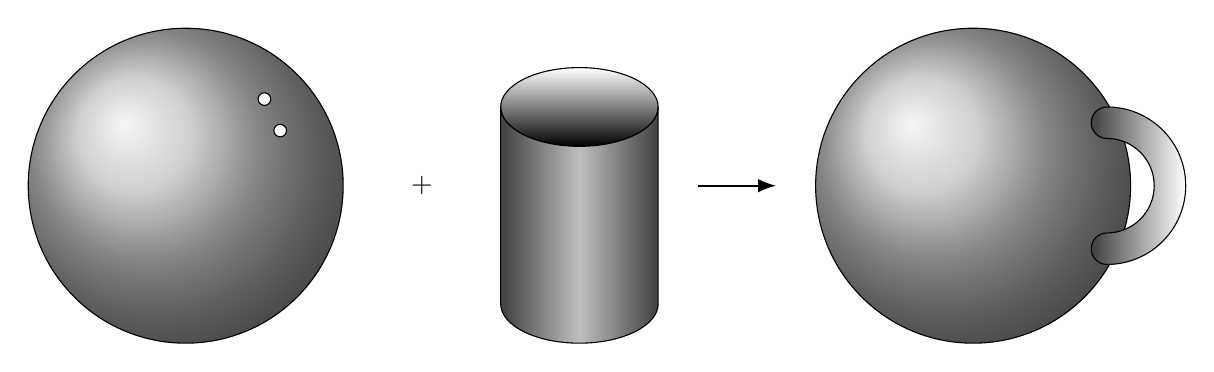
\begin{tikzpicture}
        \draw[ball color = gray!50!white] (0,0) circle (2);
        \draw[fill=white] (1,1.1) circle (0.08);
        \draw[fill=white] (1.2,0.7) circle (0.08);
        \node at (3,0) {$+$};
        \draw[bottom color=black, top color=white]
            (5,1) ellipse (1 and 0.5);
        \draw[%
            left color=gray!50!black,
            right color=gray!50!black,
            middle color=gray!50,
            shading=axis
        ]   (4,1)--(4,-1.5)
            arc(180:360:1 and 0.5)--(6,1)
            arc(360:180:1 and 0.5);
        \draw[>=Latex, ->, thick] (6.5,0)--(7.5,0);
        \draw[ball color=gray!50!white] (10,0) circle (2);
        \draw[left color=black!50!gray, right color=white, thin]
            (11.7,1) arc(90:-90:1) arc(-90:-270:0.2)
                     arc(-90:90:0.6) arc(-90:-270:0.2);
    \end{tikzpicture}
\end{document}}
                \caption{Simple Surgery Example.}
                \label{fig:surgery_theory_example_of_a_surgery}
            \end{figure}
            Recall that $S^{0}$ is two points, and that
            $D^{2}$ is the open unit disc. Then $S^{0}\times D^{2}$
            is simply two disjoint open unit discs. This is a good
            representation of the idea of the disjoint union,
            denoted $X\coprod Y$. We have:
            \begin{equation*}
                S^{0}\times{D^{2}}=D^{2}\coprod{D^{2}}
            \end{equation*}
            We can also represent a cylinder as the closed
            $S^{1}\times \overline{D}^{1}$. The codimension
            of a surgery is the dimension of the object minus
            the dimension of a surgery. So, for the surgery
            in Fig.~\ref{fig:surgery_theory_example_of_a_surgery},
            the dimension of the entire thing is $2$, the dimension
            of the surgery is $2$, so the codimension is $0$.
            This is called a Zero-Surgery. A zero-surgery takes
            out $2$ holes and connects them with a tube.
            \begin{figure}[H]
                \centering
                \captionsetup{type=figure}
                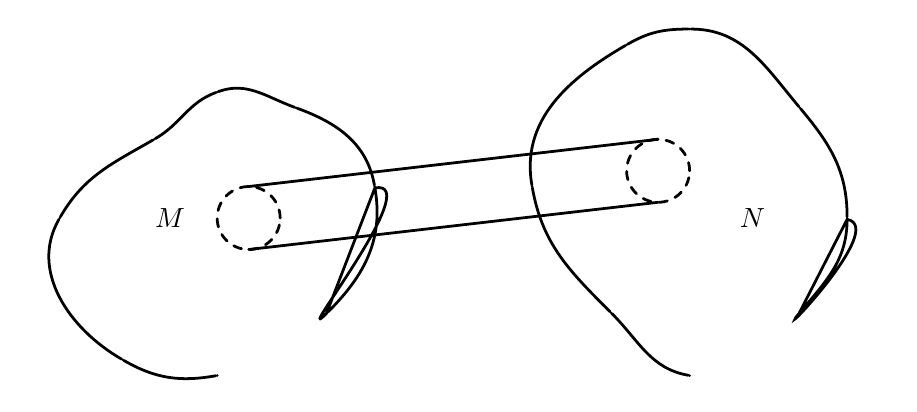
\begin{tikzpicture}[%
    scale=2,
    line width=1pt,
    line cap=round,
]
    \begin{scope}[%
        every node/.style={
            fill=black,
            circle,
            inner sep=0pt,
            outer sep=0pt
        }
    ]
        \node at (0,0) (a) {};
        \node at (-0.6,0.1) (b) {};
        \node at (-1,1) (c) {};
        \node at (-0.4,1.5) (d) {};
        \node at (0, 1.8) (e) {};
        \node at (0.5, 1.7) (f) {};
        \node at (1,1.2) (g) {};
        \node at (0.7,0.4) (h) {};
        \node at (3,0) (a1) {};
        \node at (2.5,0.4) (b1) {};
        \node at (2,1.2) (c1) {};
        \node at (2.6,2.1) (d1) {};
        \node at (3, 2.2) (e1) {};
        \node at (3.7, 1.7) (f1) {};
        \node at (4,1) (g1) {};
        \node at (3.7,0.4) (h1) {};
    \end{scope}
    \node at (-0.3,1) (i) {$M$};
    \node at (3.4,1) (i1) {$N$};
    \draw (a) to [out=-170,in=-30] (b)
              to [out=150,in=-120] (c)
              to [out=60,in=-150] (d)
              to [out=30,in=-160] (e)
              to [out=20,in=160] (f)
              to [out=-20,in=100] (g)
              to [out=-80,in=45] (h)
              to [out=-135,in=10] cycle;
    \draw (a1) to [out=170,in=-45] (b1)
               to [out=135,in=-80] (c1)
               to [out=100,in=-150] (d1)
               to [out=30,in=180] (e1)
               to [out=0,in=130] (f1)
               to [out=-50,in=90] (g1)
               to [out=-90,in=50] (h1)
               to [out=-130,in=-10] cycle;
    \draw[dashed] (0.2,1) circle (0.2);
    \draw[dashed] (2.8,1.3) circle (0.2);
    \draw (0.2,1.2) -- (2.8,1.5);
    \draw (0.2,0.8) -- (2.8,1.1);
\end{tikzpicture}
                \caption{Example of a Zero Surgery.}
                \label{fig:surgery_theory_a_zero_surgery}
            \end{figure}
            Let $\mathcal{M}^{n}$ be an $n$ dimensional manifold.
            Embed
            $S^{k}\times D^{n-k}$ into $\mathcal{M}^{n}$.
            Let $\partial(X)$ be the boundary of $X$.
            Then we have:
            \begin{align*}
                \partial(S^{k}\times {D^{n-k}})
                &=S^{k}\times{S^{n-k-1}}
                &
                \dim(S^{k+1}\times{D^{n-k-1})}
                &=\dim(S^{k}\times{D^{n-k}})=n
            \end{align*}
            Remove $\partial(S^{k}\times{D^{n-k}})$ and glue on
            $S^{k+1}\times{D}^{n-k-1}$. We alse have that
            $\partial(D^{k+1}\times{S^{n-k-1}})=S^{k}\times{S^{n-k-1}}$.
            Glue $\mathcal{M}^{n}\cup(D^{k+1}\times S^{n-k-1})$
            along $\partial(S^{k}\times{S^{n-k-1}})$.
            \begin{figure}[H]
                \centering
                \captionsetup{type=figure}
                \documentclass[crop,class=article]{standalone}
%----------------------------Preamble-------------------------------%
\usepackage{tikz}                       % Drawing/graphing tools.
\usetikzlibrary{arrows.meta}            % Latex and Stealth arrows.
%--------------------------Main Document----------------------------%
\begin{document}
    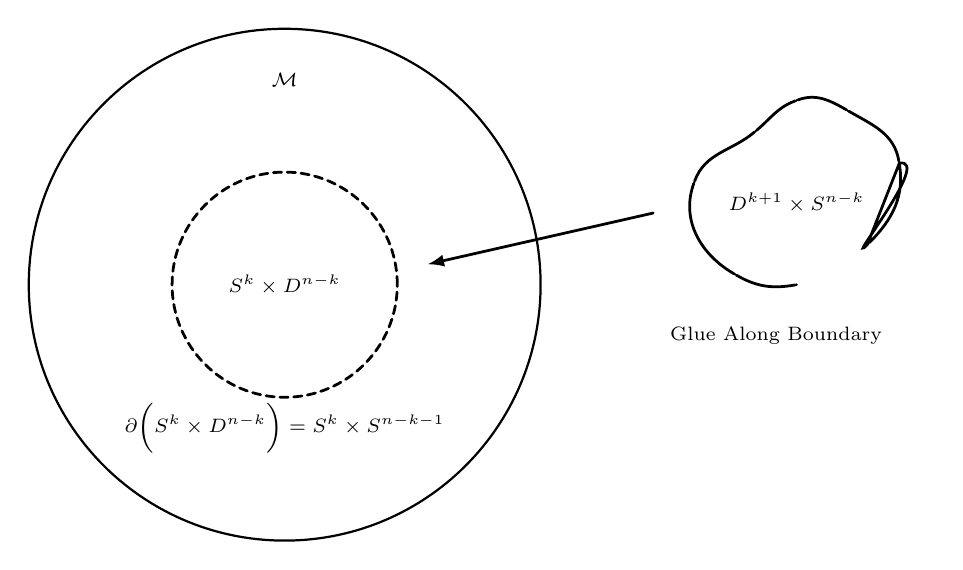
\begin{tikzpicture}[%
        font=\scriptsize,
        scale=1.3,
        line width=1pt,
        line cap=round,
        >={Latex[black]},
        every edge/.style={draw=black,very thick}
    ]
        \draw[densely dashed] (0,0) circle (1.1);
        \draw[thick] (0,0) circle (2.5);
        \node at (0,2) {$\mathcal{M}$};
        \node at (0,0) {$S^{k}\times D^{n-k}$};
        \node at (0,-1.4)
            {
                $\partial\big(S^{k}\times{D^{n-k}}\big)%
                 =S^{k}\times{S^{n-k-1}}$
            };
        \begin{scope}[%
            every node/.style={
                fill=black,
                circle,
                inner sep=0pt,
                outer sep=0pt
            }
        ]
            \node at (5,0) (a) {};
            \node at (4.4,0.1) (b) {};
            \node at (4,1) (c) {};
            \node at (4.6,1.5) (d) {};
            \node at (5, 1.8) (e) {};
            \node at (5.5, 1.7) (f) {};
            \node at (6,1.2) (g) {};
            \node at (5.7,0.4) (h) {};
        \end{scope}
        \node at (5,0.8) {$D^{k+1}\times{S^{n-k}}$};
        \draw[>=latex,->] (3.6,0.7)--(1.4,0.2);
        \node at (4.8,-0.5) {Glue Along Boundary};
        \draw (a) to [out=-170,in=-30] (b)
                  to [out=150,in=-110] (c)
                  to [out=70,in=-140] (d)
                  to [out=40,in=-160] (e)
                  to [out=20,in=150] (f)
                  to [out=-30,in=100] (g)
                  to [out=-80,in=45] (h)
                  to [out=-135,in=10] cycle;
    \end{tikzpicture}
\end{document}
                \caption[More Complicated Surgery Example.]
                        {Gluing $D^{k+1}\times S^{n-k}$ along
                         $\partial(S^{k}\times D^{n-k})$. The new manifold is
                         $\mathcal{M}^{n}\setminus(S^{k}\times%
                          D^{n-k}\coprod(D^{k+1}\times S^{n-k-1})$}
                \label{fig:surgery_theory_glueing_S_k_D_n_k_to_M}
            \end{figure}
            We now consider $k$ surgeries
            $\mathcal{M}\overset{\textrm{k-surgery}}%
                                {\longrightarrow}\mathcal{N}$.
            We have seen
            $S^{2}\overset{\textrm{0-surgery}}{\longrightarrow}T^{2}$.
            Note: $\pi_{1}(S^{2})$ is trivial, and
            $\pi_{1}(T^{2})=\mathbb{Z}^{2}$. This happens because $n<5$. When
            $n\geq{5}$, we have the following result.
            \begin{theorem}
                If $\mathcal{M}$ is an $n$ dimensional manifold, $n\geq{5}$,
                and if $\mathcal{N}$ is the result of a $k$ surgery on
                $\mathcal{M}$, then $\pi_{1}(\mathcal{M})=\pi_{1}(\mathcal{N})$.
            \end{theorem}
        \subsubsection{More On Surgery Exact Sequences}
            Recall that a surgery exact sequence looks like the following:
            \begin{equation*}
                \underset{\textrm{Group}}
                {\underbrace{L_{n+1}(\mathbb{Z}\pi_{1}\mathcal{M})}}
                \rightarrow\cdots\rightarrow
                \underset{\textrm{Not a Group}}
                {\underbrace{S^{Cat}(\mathcal{M}^{n})}}
                \rightarrow
                \underset{\textrm{Group}}
                {\underbrace{[M,G/0]}}
                \rightarrow \underset{\textrm{Group}}
                {\underbrace{L_{n}(\mathbb{Z}\pi_{1}(\mathcal{M}))}} 
            \end{equation*}
            An exact sequence of groups is of then form
            $G_{n+1}\overset{g_{n}}{\rightarrow}%
             G_{n}\rightarrow \hdots$,
            where $\Ima(g_n)=\ker(g_{n-1})$. We refine our notion of a
            surgery exact sequence:
            \begin{equation*}
                \cdots\rightarrow
                L_{n+1}(\mathbb{Z}\pi_{1}(\mathcal{M}))
                \dashrightarrow{S^{Cat}}(\mathcal{M})
                \overset{g}{\rightarrow}[M,G/o]
                \overset{\sigma}{\rightarrow}
                L_{n}(\mathbb{Z}\pi_{1}(\mathcal{M}))
            \end{equation*}
            The dotted line means
            $L_{n+1}(\mathbb{Z}\pi_{1}(\mathcal{M}))$
            acts on $S^{Cat}(\mathcal{M})$. Exact means $\Ima(g)=\ker(\sigma)$.
            Each element $f\in{[M,G/o]}$ either pulls back to $\emptyset$ or
            something non-empty. If the pullback is non-empty, you get a blob
            in $S^{Cat}(\mathcal{M})$: $f^{-1}(\{x\})$. But:
            \begin{equation}
                \bigcup_{f\in[M,G/o]}g^{-1}(\{f\})=S^{Cat}(\mathcal{M})
            \end{equation}
            This process creates a partition of $S^{Cat}(\mathcal{M})$. Now,
            $L_{n+1}(\mathbb{Z}(\pi_{1}\mathcal{M}))$ acts on
            $S^{Cat}(\mathcal{M})$ in some fashion. Partition the space into
            orbits. Exactness here means that partitioning by point inverses
            is the same as partitioning by orbits. That is, the two partitions
            are identical. See Fig.~\ref{fig:surgery_theory_partition_of_S_Cat}
            for a partitioning into orbits.
            \newpage
            \begin{figure}[H]
                \centering
                \captionsetup{type=figure}
                \documentclass[crop,class=article]{standalone}
%----------------------------Preamble-------------------------------%
%---------------------------Packages----------------------------%
\usepackage{geometry}
\geometry{b5paper, margin=1.0in}
\usepackage[T1]{fontenc}
\usepackage{graphicx, float}            % Graphics/Images.
\usepackage{natbib}                     % For bibliographies.
\bibliographystyle{agsm}                % Bibliography style.
\usepackage[french, english]{babel}     % Language typesetting.
\usepackage[dvipsnames]{xcolor}         % Color names.
\usepackage{listings}                   % Verbatim-Like Tools.
\usepackage{mathtools, esint, mathrsfs} % amsmath and integrals.
\usepackage{amsthm, amsfonts, amssymb}  % Fonts and theorems.
\usepackage{tcolorbox}                  % Frames around theorems.
\usepackage{upgreek}                    % Non-Italic Greek.
\usepackage{fmtcount, etoolbox}         % For the \book{} command.
\usepackage[newparttoc]{titlesec}       % Formatting chapter, etc.
\usepackage{titletoc}                   % Allows \book in toc.
\usepackage[nottoc]{tocbibind}          % Bibliography in toc.
\usepackage[titles]{tocloft}            % ToC formatting.
\usepackage{pgfplots, tikz}             % Drawing/graphing tools.
\usepackage{imakeidx}                   % Used for index.
\usetikzlibrary{
    calc,                   % Calculating right angles and more.
    angles,                 % Drawing angles within triangles.
    arrows.meta,            % Latex and Stealth arrows.
    quotes,                 % Adding labels to angles.
    positioning,            % Relative positioning of nodes.
    decorations.markings,   % Adding arrows in the middle of a line.
    patterns,
    arrows
}                                       % Libraries for tikz.
\pgfplotsset{compat=1.9}                % Version of pgfplots.
\usepackage[font=scriptsize,
            labelformat=simple,
            labelsep=colon]{subcaption} % Subfigure captions.
\usepackage[font={scriptsize},
            hypcap=true,
            labelsep=colon]{caption}    % Figure captions.
\usepackage[pdftex,
            pdfauthor={Ryan Maguire},
            pdftitle={Mathematics and Physics},
            pdfsubject={Mathematics, Physics, Science},
            pdfkeywords={Mathematics, Physics, Computer Science, Biology},
            pdfproducer={LaTeX},
            pdfcreator={pdflatex}]{hyperref}
\hypersetup{
    colorlinks=true,
    linkcolor=blue,
    filecolor=magenta,
    urlcolor=Cerulean,
    citecolor=SkyBlue
}                           % Colors for hyperref.
\usepackage[toc,acronym,nogroupskip,nopostdot]{glossaries}
\usepackage{glossary-mcols}
%------------------------Theorem Styles-------------------------%
\theoremstyle{plain}
\newtheorem{theorem}{Theorem}[section]

% Define theorem style for default spacing and normal font.
\newtheoremstyle{normal}
    {\topsep}               % Amount of space above the theorem.
    {\topsep}               % Amount of space below the theorem.
    {}                      % Font used for body of theorem.
    {}                      % Measure of space to indent.
    {\bfseries}             % Font of the header of the theorem.
    {}                      % Punctuation between head and body.
    {.5em}                  % Space after theorem head.
    {}

% Italic header environment.
\newtheoremstyle{thmit}{\topsep}{\topsep}{}{}{\itshape}{}{0.5em}{}

% Define environments with italic headers.
\theoremstyle{thmit}
\newtheorem*{solution}{Solution}

% Define default environments.
\theoremstyle{normal}
\newtheorem{example}{Example}[section]
\newtheorem{definition}{Definition}[section]
\newtheorem{problem}{Problem}[section]

% Define framed environment.
\tcbuselibrary{most}
\newtcbtheorem[use counter*=theorem]{ftheorem}{Theorem}{%
    before=\par\vspace{2ex},
    boxsep=0.5\topsep,
    after=\par\vspace{2ex},
    colback=green!5,
    colframe=green!35!black,
    fonttitle=\bfseries\upshape%
}{thm}

\newtcbtheorem[auto counter, number within=section]{faxiom}{Axiom}{%
    before=\par\vspace{2ex},
    boxsep=0.5\topsep,
    after=\par\vspace{2ex},
    colback=Apricot!5,
    colframe=Apricot!35!black,
    fonttitle=\bfseries\upshape%
}{ax}

\newtcbtheorem[use counter*=definition]{fdefinition}{Definition}{%
    before=\par\vspace{2ex},
    boxsep=0.5\topsep,
    after=\par\vspace{2ex},
    colback=blue!5!white,
    colframe=blue!75!black,
    fonttitle=\bfseries\upshape%
}{def}

\newtcbtheorem[use counter*=example]{fexample}{Example}{%
    before=\par\vspace{2ex},
    boxsep=0.5\topsep,
    after=\par\vspace{2ex},
    colback=red!5!white,
    colframe=red!75!black,
    fonttitle=\bfseries\upshape%
}{ex}

\newtcbtheorem[auto counter, number within=section]{fnotation}{Notation}{%
    before=\par\vspace{2ex},
    boxsep=0.5\topsep,
    after=\par\vspace{2ex},
    colback=SeaGreen!5!white,
    colframe=SeaGreen!75!black,
    fonttitle=\bfseries\upshape%
}{not}

\newtcbtheorem[use counter*=remark]{fremark}{Remark}{%
    fonttitle=\bfseries\upshape,
    colback=Goldenrod!5!white,
    colframe=Goldenrod!75!black}{ex}

\newenvironment{bproof}{\textit{Proof.}}{\hfill$\square$}
\tcolorboxenvironment{bproof}{%
    blanker,
    breakable,
    left=3mm,
    before skip=5pt,
    after skip=10pt,
    borderline west={0.6mm}{0pt}{green!80!black}
}

\AtEndEnvironment{lexample}{$\hfill\textcolor{red}{\blacksquare}$}
\newtcbtheorem[use counter*=example]{lexample}{Example}{%
    empty,
    title={Example~\theexample},
    boxed title style={%
        empty,
        size=minimal,
        toprule=2pt,
        top=0.5\topsep,
    },
    coltitle=red,
    fonttitle=\bfseries,
    parbox=false,
    boxsep=0pt,
    before=\par\vspace{2ex},
    left=0pt,
    right=0pt,
    top=3ex,
    bottom=1ex,
    before=\par\vspace{2ex},
    after=\par\vspace{2ex},
    breakable,
    pad at break*=0mm,
    vfill before first,
    overlay unbroken={%
        \draw[red, line width=2pt]
            ([yshift=-1.2ex]title.south-|frame.west) to
            ([yshift=-1.2ex]title.south-|frame.east);
        },
    overlay first={%
        \draw[red, line width=2pt]
            ([yshift=-1.2ex]title.south-|frame.west) to
            ([yshift=-1.2ex]title.south-|frame.east);
    },
}{ex}

\AtEndEnvironment{ldefinition}{$\hfill\textcolor{Blue}{\blacksquare}$}
\newtcbtheorem[use counter*=definition]{ldefinition}{Definition}{%
    empty,
    title={Definition~\thedefinition:~{#1}},
    boxed title style={%
        empty,
        size=minimal,
        toprule=2pt,
        top=0.5\topsep,
    },
    coltitle=Blue,
    fonttitle=\bfseries,
    parbox=false,
    boxsep=0pt,
    before=\par\vspace{2ex},
    left=0pt,
    right=0pt,
    top=3ex,
    bottom=0pt,
    before=\par\vspace{2ex},
    after=\par\vspace{1ex},
    breakable,
    pad at break*=0mm,
    vfill before first,
    overlay unbroken={%
        \draw[Blue, line width=2pt]
            ([yshift=-1.2ex]title.south-|frame.west) to
            ([yshift=-1.2ex]title.south-|frame.east);
        },
    overlay first={%
        \draw[Blue, line width=2pt]
            ([yshift=-1.2ex]title.south-|frame.west) to
            ([yshift=-1.2ex]title.south-|frame.east);
    },
}{def}

\AtEndEnvironment{ltheorem}{$\hfill\textcolor{Green}{\blacksquare}$}
\newtcbtheorem[use counter*=theorem]{ltheorem}{Theorem}{%
    empty,
    title={Theorem~\thetheorem:~{#1}},
    boxed title style={%
        empty,
        size=minimal,
        toprule=2pt,
        top=0.5\topsep,
    },
    coltitle=Green,
    fonttitle=\bfseries,
    parbox=false,
    boxsep=0pt,
    before=\par\vspace{2ex},
    left=0pt,
    right=0pt,
    top=3ex,
    bottom=-1.5ex,
    breakable,
    pad at break*=0mm,
    vfill before first,
    overlay unbroken={%
        \draw[Green, line width=2pt]
            ([yshift=-1.2ex]title.south-|frame.west) to
            ([yshift=-1.2ex]title.south-|frame.east);},
    overlay first={%
        \draw[Green, line width=2pt]
            ([yshift=-1.2ex]title.south-|frame.west) to
            ([yshift=-1.2ex]title.south-|frame.east);
    }
}{thm}

%--------------------Declared Math Operators--------------------%
\DeclareMathOperator{\adjoint}{adj}         % Adjoint.
\DeclareMathOperator{\Card}{Card}           % Cardinality.
\DeclareMathOperator{\curl}{curl}           % Curl.
\DeclareMathOperator{\diam}{diam}           % Diameter.
\DeclareMathOperator{\dist}{dist}           % Distance.
\DeclareMathOperator{\Div}{div}             % Divergence.
\DeclareMathOperator{\Erf}{Erf}             % Error Function.
\DeclareMathOperator{\Erfc}{Erfc}           % Complementary Error Function.
\DeclareMathOperator{\Ext}{Ext}             % Exterior.
\DeclareMathOperator{\GCD}{GCD}             % Greatest common denominator.
\DeclareMathOperator{\grad}{grad}           % Gradient
\DeclareMathOperator{\Ima}{Im}              % Image.
\DeclareMathOperator{\Int}{Int}             % Interior.
\DeclareMathOperator{\LC}{LC}               % Leading coefficient.
\DeclareMathOperator{\LCM}{LCM}             % Least common multiple.
\DeclareMathOperator{\LM}{LM}               % Leading monomial.
\DeclareMathOperator{\LT}{LT}               % Leading term.
\DeclareMathOperator{\Mod}{mod}             % Modulus.
\DeclareMathOperator{\Mon}{Mon}             % Monomial.
\DeclareMathOperator{\multideg}{mutlideg}   % Multi-Degree (Graphs).
\DeclareMathOperator{\nul}{nul}             % Null space of operator.
\DeclareMathOperator{\Ord}{Ord}             % Ordinal of ordered set.
\DeclareMathOperator{\Prin}{Prin}           % Principal value.
\DeclareMathOperator{\proj}{proj}           % Projection.
\DeclareMathOperator{\Refl}{Refl}           % Reflection operator.
\DeclareMathOperator{\rk}{rk}               % Rank of operator.
\DeclareMathOperator{\sgn}{sgn}             % Sign of a number.
\DeclareMathOperator{\sinc}{sinc}           % Sinc function.
\DeclareMathOperator{\Span}{Span}           % Span of a set.
\DeclareMathOperator{\Spec}{Spec}           % Spectrum.
\DeclareMathOperator{\supp}{supp}           % Support
\DeclareMathOperator{\Tr}{Tr}               % Trace of matrix.
%--------------------Declared Math Symbols--------------------%
\DeclareMathSymbol{\minus}{\mathbin}{AMSa}{"39} % Unary minus sign.
%------------------------New Commands---------------------------%
\DeclarePairedDelimiter\norm{\lVert}{\rVert}
\DeclarePairedDelimiter\ceil{\lceil}{\rceil}
\DeclarePairedDelimiter\floor{\lfloor}{\rfloor}
\newcommand*\diff{\mathop{}\!\mathrm{d}}
\newcommand*\Diff[1]{\mathop{}\!\mathrm{d^#1}}
\renewcommand*{\glstextformat}[1]{\textcolor{RoyalBlue}{#1}}
\renewcommand{\glsnamefont}[1]{\textbf{#1}}
\renewcommand\labelitemii{$\circ$}
\renewcommand\thesubfigure{%
    \arabic{chapter}.\arabic{figure}.\arabic{subfigure}}
\addto\captionsenglish{\renewcommand{\figurename}{Fig.}}
\numberwithin{equation}{section}

\renewcommand{\vector}[1]{\boldsymbol{\mathrm{#1}}}

\newcommand{\uvector}[1]{\boldsymbol{\hat{\mathrm{#1}}}}
\newcommand{\topspace}[2][]{(#2,\tau_{#1})}
\newcommand{\measurespace}[2][]{(#2,\varSigma_{#1},\mu_{#1})}
\newcommand{\measurablespace}[2][]{(#2,\varSigma_{#1})}
\newcommand{\manifold}[2][]{(#2,\tau_{#1},\mathcal{A}_{#1})}
\newcommand{\tanspace}[2]{T_{#1}{#2}}
\newcommand{\cotanspace}[2]{T_{#1}^{*}{#2}}
\newcommand{\Ckspace}[3][\mathbb{R}]{C^{#2}(#3,#1)}
\newcommand{\funcspace}[2][\mathbb{R}]{\mathcal{F}(#2,#1)}
\newcommand{\smoothvecf}[1]{\mathfrak{X}(#1)}
\newcommand{\smoothonef}[1]{\mathfrak{X}^{*}(#1)}
\newcommand{\bracket}[2]{[#1,#2]}

%------------------------Book Command---------------------------%
\makeatletter
\renewcommand\@pnumwidth{1cm}
\newcounter{book}
\renewcommand\thebook{\@Roman\c@book}
\newcommand\book{%
    \if@openright
        \cleardoublepage
    \else
        \clearpage
    \fi
    \thispagestyle{plain}%
    \if@twocolumn
        \onecolumn
        \@tempswatrue
    \else
        \@tempswafalse
    \fi
    \null\vfil
    \secdef\@book\@sbook
}
\def\@book[#1]#2{%
    \refstepcounter{book}
    \addcontentsline{toc}{book}{\bookname\ \thebook:\hspace{1em}#1}
    \markboth{}{}
    {\centering
     \interlinepenalty\@M
     \normalfont
     \huge\bfseries\bookname\nobreakspace\thebook
     \par
     \vskip 20\p@
     \Huge\bfseries#2\par}%
    \@endbook}
\def\@sbook#1{%
    {\centering
     \interlinepenalty \@M
     \normalfont
     \Huge\bfseries#1\par}%
    \@endbook}
\def\@endbook{
    \vfil\newpage
        \if@twoside
            \if@openright
                \null
                \thispagestyle{empty}%
                \newpage
            \fi
        \fi
        \if@tempswa
            \twocolumn
        \fi
}
\newcommand*\l@book[2]{%
    \ifnum\c@tocdepth >-3\relax
        \addpenalty{-\@highpenalty}%
        \addvspace{2.25em\@plus\p@}%
        \setlength\@tempdima{3em}%
        \begingroup
            \parindent\z@\rightskip\@pnumwidth
            \parfillskip -\@pnumwidth
            {
                \leavevmode
                \Large\bfseries#1\hfill\hb@xt@\@pnumwidth{\hss#2}
            }
            \par
            \nobreak
            \global\@nobreaktrue
            \everypar{\global\@nobreakfalse\everypar{}}%
        \endgroup
    \fi}
\newcommand\bookname{Book}
\renewcommand{\thebook}{\texorpdfstring{\Numberstring{book}}{book}}
\providecommand*{\toclevel@book}{-2}
\makeatother
\titleformat{\part}[display]
    {\Large\bfseries}
    {\partname\nobreakspace\thepart}
    {0mm}
    {\Huge\bfseries}
\titlecontents{part}[0pt]
    {\large\bfseries}
    {\partname\ \thecontentslabel: \quad}
    {}
    {\hfill\contentspage}
\titlecontents{chapter}[0pt]
    {\bfseries}
    {\chaptername\ \thecontentslabel:\quad}
    {}
    {\hfill\contentspage}
\newglossarystyle{longpara}{%
    \setglossarystyle{long}%
    \renewenvironment{theglossary}{%
        \begin{longtable}[l]{{p{0.25\hsize}p{0.65\hsize}}}
    }{\end{longtable}}%
    \renewcommand{\glossentry}[2]{%
        \glstarget{##1}{\glossentryname{##1}}%
        &\glossentrydesc{##1}{~##2.}
        \tabularnewline%
        \tabularnewline
    }%
}
\newglossary[not-glg]{notation}{not-gls}{not-glo}{Notation}
\newcommand*{\newnotation}[4][]{%
    \newglossaryentry{#2}{type=notation, name={\textbf{#3}, },
                          text={#4}, description={#4},#1}%
}
%--------------------------LENGTHS------------------------------%
% Spacings for the Table of Contents.
\addtolength{\cftsecnumwidth}{1ex}
\addtolength{\cftsubsecindent}{1ex}
\addtolength{\cftsubsecnumwidth}{1ex}
\addtolength{\cftfignumwidth}{1ex}
\addtolength{\cfttabnumwidth}{1ex}

% Indent and paragraph spacing.
\setlength{\parindent}{0em}
\setlength{\parskip}{0em}
%--------------------------Main Document----------------------------%
\begin{document}
    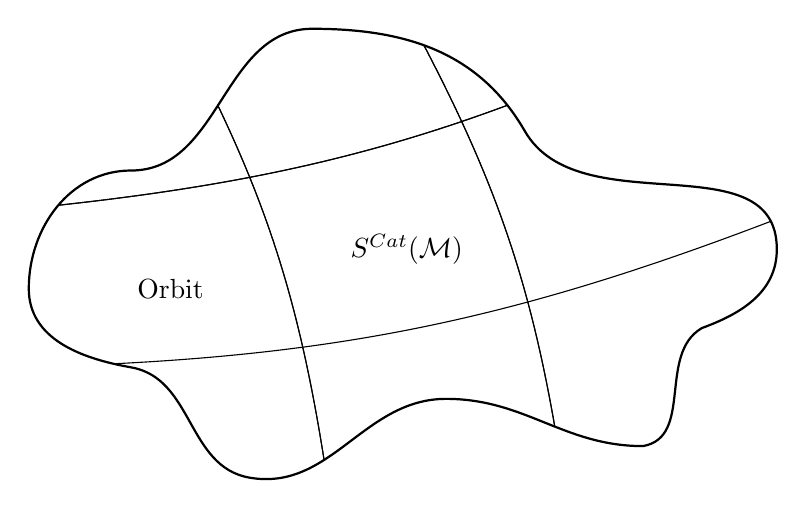
\begin{tikzpicture}
        \draw[line width=0.8pt]
            (0.2,2.5) to[out=-90,in=170]
            (1.5,1.5) to[out=-10,in=170]
            (3,0.1) to[out=-10,in=180]
            (5.5,1.1) to[out=0,in=180]
            (8,0.5) to[out=10,in=-150]
            (8.75,2) to[out=20,in=-90]
            (9.7,3) to[out=90,in=-60]
            (6.5,4.5) to[out=120,in=0]
            (3.8,5.8) to[out=180,in=0]
            (1.5,4) to[out=180,in=90] cycle;
        \clip (0.2,2.5) to[out=-90,in=170] (1.5,1.5)
                        to[out=-10,in=170] (3,0.1)
                        to[out=-10,in=180] (5.5,1.1)
                        to[out=0,in=180] (8,0.5)
                        to[out=10,in=-150] (8.75,2)
                        to[out=20,in=-90] (9.7,3)
                        to[out=90,in=-60] (6.5,4.5)
                        to[out=120,in=0] (3.8,5.8)
                        to[out=180,in=0] (1.5,4)
                        to[out=180,in=90] cycle;
        \draw (4,0) to[bend right=10] (2,6) to (5,6)
                    to [bend left=10] (7,0) to cycle;
        \draw (7,0) to[bend right=10] (5,6) to (10,6)
                    to (10,0) to cycle;
        \draw (0,1.5) to (0,3.5) to [bend right=10] (9,6)
                      to (10,6) to (10,3.5) to [bend left=10] cycle;
        \draw (0,0) to (4,0) to[bend right=10] (2,6)
                    to (0,6) to (0,0) to cycle;
        \draw (0,6) to (0,3.5) to[bend right=10] (9,6)
                    to (0,6) to cycle;
        \node at (2,2.5) {Orbit};  
        \node at (5,3) {$S^{Cat}(\mathcal{M})$};
    \end{tikzpicture}
\end{document}
                \caption{Partition of $S^{Cat}(\mathcal{M})$.}
                \label{fig:surgery_theory_partition_of_S_Cat}
            \end{figure}
            The next object to talk about is
            $L_{n}(\mathbb{Z}\pi_{1}(\mathcal{M}))$.
            These are called Wall groups. They are difficult to compute,
            but there are some facts that are known about them:
            \begin{itemize}
                \item Wall groups only have 2-torsion.
                \begin{itemize}
                    \item 2-torsion means that elements
                          of finite order have order $2$.
                    \item This implies the groups are Abelian.
                \end{itemize}
                \item They can be orientable or not.
                \begin{itemize}
                    \item $L_{n}(\mathbb{Z}\pi_{1}(\mathcal{M})^{\pm})$
                           indicates orientable or not.
                \end{itemize}
            \end{itemize}
    \subsection{Lecture 3: Vector Bundles}
        \subsubsection{Group Rings}
            \begin{definition}
                If $G$ is a group and $R$ is a ring, then the group ring $RG$
                is the collection of all finite linear combinations
                (Formal Sums): $r_{1}g_{1}+\hdots+r_{n}g_{n}$, where
                $r_{k}\in{R}$ and $g_{k}\in{G}$.
            \end{definition}
            \begin{example}
                If $G$ is a group, and
                $\mathbb{Z}G=\{\sum_{k=0}^{n}n_{k}g_{k}:%
                 n_{k}\in\mathbb{Z},g_{k}\in{G}\}$, then $\mathbb{Z}G$ is a
                group ring. This is a special group ring, denoted
                $\textrm{SP}_{\mathbb{Z}}(G)$.
            \end{example}
            \begin{theorem}
                If $R$ is a ring and $G$ is a group, then
                the group ring $RG$ is a ring.
            \end{theorem}
            From the previous lecture we saw that
            $L_{n+1}(\mathbb{Z}\pi_{1}(\mathcal{M}))$ is a group. But from the
            previous theorem, we have that $\mathbb{Z}\pi_{1}(\mathcal{M})$ is
            a ring. So, we may thing of the $L_{n}$ as a \textit{Functor}:
            $L_{n}:\textrm{Rings}\rightarrow\textrm{Groups}$.
            To recap the notation, $S(\mathcal{M})$ is the Surgery Structure
            Set on the manifold $\mathcal{M}$, and
            $L_{n}(\mathbb{Z}\pi_{1}(\mathcal{M}))$ is a Wall Group.
        \subsubsection{Matrices and Vector Bundles}
            The next monster we need to understand in the
            Surgery Exact Sequence is the
            $[\mathcal{M},G/o]$ that keep appearing.
            First, a quick recap on some notions in
            linear algebra.
            \begin{definition}
                An orthogonal matrix is an invertible
                square matrix $A$ such that
                $A^{T}=A^{-1}$
            \end{definition}
            Let $\mathcal{O}(n)$ be the group of $n\times{n}$ orthogonal
            matrices. There is a simple map then from
            $\mathcal{O}(n)$ to $\mathcal{O}(n+1)$,
            $\psi_{n}:\mathcal{O}(n)\rightarrow\mathcal{O}(n+1)$,
            defined by:
            \begin{equation*}
                \psi_{n}(A)=
                \left[%
                    \begin{array}{c|c}
                        A&0\\
                        \hline
                        0&1
                    \end{array}
                \right]
            \end{equation*}
            We can also define a map
            $\varphi_{nm}:%
             \mathcal{O}(n)\times\mathcal{O}(m)%
             \rightarrow\mathcal{O}(n+m)$ defined
            by:
            \begin{equation*}
                \varphi_{nm}(A,B)=
                \left[%
                    \begin{array}{c|c}
                        A&0\\
                        \hline
                        0&B
                    \end{array}
                \right]
            \end{equation*}
            This is, in general, not a bijection.
            From this we can create a sequence:
            \begin{equation*}
                \mathcal{O}(1)
                \overset{\psi_{1}}{\longrightarrow}\mathcal{O}(2)
                \overset{\psi_{2}}{\longrightarrow}\mathcal{O}(3)
                \overset{\psi_{3}}{\longrightarrow}\mathcal{O}(4)
                \overset{\psi_{4}}{\longrightarrow}\cdots
                \mathcal{O}(n)\overset{\psi_{n}}{\longrightarrow}\cdots
            \end{equation*}
            We can then define $\mathcal{O}$ as the
            \textit{Direct Limit} of this sequence:
            \begin{equation*}
                \mathcal{O}=\underset{n\rightarrow\infty}{\lim}\mathcal{O}(n)
            \end{equation*}
            Now, let $\mathcal{M}$ be a manifold. An $n$ dimensional vector
            bundle is a map $P:E\rightarrow\mathcal{M}$ such that, for each
            point $x\in\mathcal{M}$, the \textit{fiber} of $x$, the pre-image
            $p^{-1}(x)$, is homeomorphic to $\mathbb{R}^{n}$.
            \begin{definition}
                The fiber of a point $y$ in a set $Y$ under the map
                $f:X\rightarrow{Y}$ is the pre-image $f^{-1}(y)\subset{X}$.
            \end{definition}
            \begin{definition}
                A real $n$ dimensional vector bundle on a manifold $\mathcal{M}$
                is a manifold $E$ and a continuous map
                $p:E\rightarrow\mathcal{M}$ such that, for all
                $x\in\mathcal{M}$, the fiber of $x$ is homeomorphic to
                $\mathbb{R}^{n}$ and there exists an open set $\mathcal{U}$
                such that $x\in\mathcal{U}$ and $p^{-1}(\mathcal{U})$ is
                homeomorphic to $\mathcal{U}\times\mathbb{R}^{n}$
            \end{definition}
            The requirement that there is an open neighborhood $\mathcal{U}_{x}$
            for all $x$ such that $p^{-1}(\mathcal{U})$ is homeomoprhic to
            $\mathcal{U}_{x}\times\mathbb{R}^{n}$ is called
            \textit{local triviality}. There is another notion called
            \textit{global triviality}.
            \begin{example}
                A classic example is a cylinder with a disk (Or the boundary of
                a cylinder with the circle). Given a point $(x,y,z)$ in the
                cylinder, collapse this (Or project it) down onto the $xy$
                plane by the map $p(x,y,z)=(x,y)$. This is continuous, and is
                an example of a vector bundle:
                $(D^{1},D^{1}\times\mathbb{R},p)$. The pre-image, or fiber, of
                any point in $D^{1}$ is a line, which is certainly homeomorphic
                to $\mathbb{R}$. Again, taking any point $x$ and looking at an
                open ball about that point that is entirely contained within
                $D^{1}$, the pre-image $p^{-1}(B_{r}(x))$ is another cylinder,
                which is homeomorphic to $\mathbb{R}^{3}$, which is itself
                homeomorphic to $B_{r}(x)\times\mathbb{R}^{1}$. The fibers of
                $x$ and $\mathcal{U}$ are shown in
                Fig.~\ref{fig:Simple_Vector_Bundle_Cylinder_to_Disk}
            \end{example}
            \begin{figure}[H]
                \centering
                \captionsetup{type=figure}
                \documentclass[crop,class=article]{standalone}
%----------------------------Preamble-------------------------------%
\usepackage{tikz}                       % Drawing/graphing tools.
%--------------------------Main Document----------------------------%
\begin{document}
    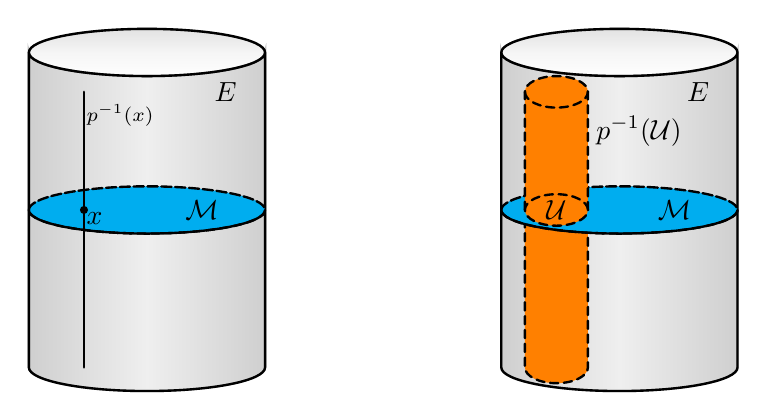
\begin{tikzpicture}[%
        line width=0.3mm,
        line cap=round,
    ]
        \draw[%
            left color=gray!50!black,
            right color=gray!50!black,
            middle color=gray!50,
            shading=axis,
            opacity=0.25
        ]   (1.5,0) to (1.5,4) arc (360:180:1.5cm and 0.3cm)
                    to (-1.5,0) arc (180:360:1.5cm and 0.3cm);
        \draw[%
            top color=gray!90!,
            bottom color=gray!2,
            middle color=gray!30,
            shading=axis,
            opacity=0.25
        ]   (0,4) circle (1.5cm and 0.3cm);
        \draw (-1.5,4) to (-1.5,0) arc (180:360:1.5cm and 0.3cm)
                       to (1.5,4) (0,4) circle (1.5cm and 0.3cm);
        \draw[fill=cyan,densely dashed]
            (-1.5,2) arc (180:0:1.5cm and 0.3cm) 
                     arc (360:0:1.5cm and 0.3cm);
        \draw (-1.5,2) arc (180:360:1.5cm and 0.3cm);
        \node[%
            circle,
            fill=black,
            draw=black,
            inner sep=0pt,
            minimum size=2pt
        ]   at (-0.8,2) {};
        \node at (-0.9,2.1) [below right] {$x$};
        \node at (0.7,2) {$\mathcal{M}$};
        \node at (1,3.5) {$E$};
        \node at (-0.9,3.2) [right] {\scriptsize{$p^{-1}(x)$}};
        \draw (-0.8,0) to (-0.8,3.5);

        % Shift for the second cylinder.
        \begin{scope}[xshift=6cm]
            \draw[%
                left color=gray!50!black,
                right color=gray!50!black,
                middle color=gray!50,
                shading=axis,
                opacity=0.25
            ]   (1.5,0) to (1.5,4) arc (360:180:1.5cm and 0.3cm)
                        to (-1.5,0) arc (180:360:1.5cm and 0.3cm);
            \draw[%
                top color=gray!90!,
                bottom color=gray!2,
                middle color=gray!30,
                shading=axis,
                opacity=0.25
            ]   (0,4) circle (1.5cm and 0.3cm);
            \draw (-1.5,4) to (-1.5,0) arc (180:360:1.5cm and 0.3cm)
                           to (1.5,4) (0,4) circle (1.5cm and 0.3cm);
            \draw[densely dashed, fill=orange]
                (-0.4,2) to (-0.4,0) arc (360:180:4mm and 2mm)
                         to (-1.2,2);
            \draw[fill=cyan,densely dashed]
                (-1.5,2) arc (180:0:1.5cm and 0.3cm) 
                         arc (360:0:1.5cm and 0.3cm);
            \draw (-1.5,2) arc (180:360:1.5cm and 0.3cm);
            \draw[densely dashed, fill=orange]
                (-1.2,2) to (-1.2,3.5) arc (180:0:4mm and 2mm)
                         to (-0.4,2);
            \draw[densely dashed,fill=orange]
                (-0.8,2) circle (4mm and 2mm);
            \draw[densely dashed]
                (-1.2,3.5) arc (180:360:4mm and 2mm);
            \node at (-0.8,2) {$\mathcal{U}$};
            \node at (0.7,2) {$\mathcal{M}$};
            \node at (1,3.5) {$E$};
            \node at (0.25,3) {$p^{-1}(\mathcal{U})$};
        \end{scope}
    \end{tikzpicture}
\end{document}
                \caption{Example of a Vector Bundle:
                         $(D^{1},D^{1}\times\mathbb{R},p)$.}
                \label{fig:Simple_Vector_Bundle_Cylinder_to_Disk}
            \end{figure}
            \begin{example}
                If $\mathcal{M}$ is a manifold,
                $E=\mathcal{M}\times\mathbb{R}^{n}$, and if
                $p:E\rightarrow\mathcal{M}$ is defined by $p(x,\mathbf{y})=x$
                for all $(x,\mathbf{y})\in\mathcal{M}\times\mathbb{R}^{n}$,
                then $(E,\mathcal{M},p)$ is a vector bundle. This is called
                the trivial $n$ dimensional vector bundle of $\mathbb{R}^{n}$.
                The fibers of points $x\in\mathcal{M}$ are $\mathbb{R}^{n}$,
                which is homeomorphic to $\mathbb{R}^{n}$. Given any open set
                $\mathcal{U}$ containing $x$, the pre-image is
                $\mathcal{U}\times\mathbb{R}^{n}$.
            \end{example}
            \begin{example}
                The M\"{o}bius strip can be seen as a vector bundle
                $S^{1}\times[0,1]\rightarrow[0,1]$ where the map
                $(x,t)\rightarrow{x}$ is by a ``twist.'' This is a
                non-oreientable bundle which is non-trivial. It has local
                triviality, but no global triviality.
            \end{example}
            \begin{figure}[H]
                \centering
                \captionsetup{type=figure}
                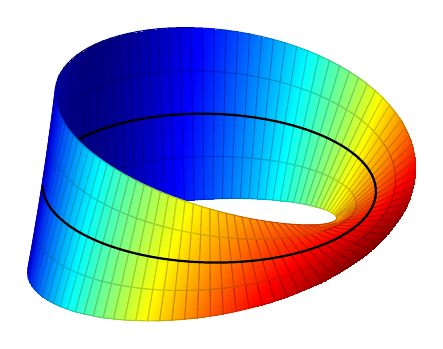
\begin{tikzpicture}
    \begin{axis}[
        hide axis,
        view={40}{40}
    ]
        \addplot3[%
            surf,
            shader=faceted interp,
            point meta=x,
            colormap/jet,
            samples=100,
            samples y=5,
            domain=0:360,
            y domain=-0.5:0.5
        ]   ({(1+0.5*y*cos(x/2)))*cos(x)},
             {(1+0.5*y*cos(x/2)))*sin(x)},
             {0.5*y*sin(x/2)});
        \addplot3[%
            samples=100,
            domain=-140:180,
            samples y=0,
            thick,
            line cap=round
        ]   ({cos(x)},{sin(x)},{0});
    \end{axis}
\end{tikzpicture}
                \caption{M\"{o}bius Strip.}
                \label{fig:Surgery_Theory_Mobius_Strip_Vector_Bundle}
            \end{figure}
            Returning to our discussion of orthogonal matrices,
            $\mathcal{O}(n)$ is a group under matrix multiplication.
            The matrix $I_{n}$ is orthogonal, and if $A$ is orthogonal,
            then $(A^{-1})^{T}=(A^{T})^{T}=A$. But $(A^{-1})^{-1}=A$,
            and thus $A^{-1}$ is orthogonal as well. Thus we have
            an identity, associativity, and closure of inverses.
            Therefore $\mathcal{O}(n)$ is a group. This group can
            act on the set of $n$ dimensional vectors in
            $\mathbb{R}^{n}$ by the map
            $(A,\mathbf{v})\rightarrow{A\mathbf{v}}$,
            for all $A\in\mathcal{O}(n),\mathbf{v}\in\mathbb{R}^{n}$.
            Thus, we have the $\mathcal{O}(n)$ acts over the fibers
            of an $n$ dimensional real vector bundle
            $(E,\mathcal{M},p)$. $\mathcal{O}(1)$ is the identity.
            That is, the ``Do nothing,'' action on a 1 dimensional
            vector bundle. $\mathcal{O}(2)$ can perform
            \textit{reflections} and \textit{rotations} on the
            fibers. Endowed with this action, any real
            vector bundle of dimension $n$ is an example of
            a \textit{principal $\mathcal{O}(n)$ bundle}.
            If $g\in\mathcal{O}(n)$ and $v\in{E}$,
            then $p(gv)=g(p(v)$.
        \subsubsection{Principal G-Bundles}
            If $G$ is a group, and if $X$ is a
            topogolical space, then there is a
            structure/notion of a
            \textit{principal G-Bundle} on $X$.
            That is, $X$ has some bundle over it
            (The space $E$ from our previous discussion),
            and $G$ acts on the fibers of $X$. This is
            denoted $\Prin_{G}(X)$.
            \par\hfill\par
            Construction by John Milnor, Classifying space.
            No idea why I wrote this...
            \par\hfill\par
            If $G$ is a group, there is a complex (space) $BG$
            such that we may form the set:
            \begin{equation*}
                [\mathcal{M},BG]
                =\{f:\mathcal{M}\rightarrow{BG}\}/Homotopy
            \end{equation*}
            That is, the set of continuous maps from $\mathcal{M}$ to
            $BG$ modded out by homotopy. Two maps are equivalent if they
            are homotopic.
            \begin{theorem}
                There is a continuous surjective function
                $f:\Prin_{G}(\mathcal{M})\rightarrow%
                 [\mathcal{M},BG]$.
            \end{theorem}
            Elaborating more on the $BG$,
            $B$ is a \textit{functor}
            $B:\textrm{Groups}\rightarrow\textrm{Spaces}$.
            If $G$ is a finitely presented group,
            then $\pi_{1}(BG)=G$, and more over,
            for all $n\geq{2}$,
            $\pi_{n}(BG)=0$. That is, $\pi_{n}(BG)$
            is the trivial group for all $n\geq{2}$.
            $\pi_{1}(X)$ ca be seen as the
            \textit{homotopy class} of $[S^{1},X]$.
            $\pi_{n}$ the homotopy class for
            $[S^{n},X]$.
            \begin{example}
                $\pi_{1}(B\mathbb{Z})=\mathbb{Z}$.
                For all $n\geq{2}$,
                $\pi_{n}(B\mathbb{Z})=0$.
                Thus $B\mathbb{Z}$ is homotopy
                equivalent to $S^{1}$.
            \end{example}
        \subsubsection{Covering Spaces}
            \begin{definition}
                A covering space of a topological space $X$ is a space $E$ such
                that there exists a continuous surjection $p:E\rightarrow{X}$
                such that for all $x\in{X}$, there is an open set $\mathcal{U}$
                such that $x\in\mathcal{U}$ such that there exists a set of
                disjoint open sets $E_{r}\subset{E}$ where
                $p^{-1}(\mathcal{U})=\cup_{r}E_{r}$ and for all $r$, $p$ is a
                homeomorphism between $E_{r}$ and $\mathcal{U}$.
            \end{definition}
            \begin{example}
                The first example is $S^{1}$ and $\mathbb{R}$. Define the map
                $p:\mathbb{R}\rightarrow{S^{1}}$ by $p(x)=\exp(2\pi{i}x)$. This
                ``wraps,'' the real line around the circle over and over again.
                Given a point $y\in{S^{1}}$, the pre-image, or fiber, of $y$
                with respect to $p$ is $\{x+n:n\in\mathbb{Z}\}$ for some
                $x\in[0,1)$. Given a small enough neighborhood around $y$, the
                pre-image is of the form
                $\{x+n-\varepsilon,x+n+\varepsilon:n\in\mathbb{Z}\}$,
                which is a bunch of copies of $(0,1)$, or a bunch
                of copies of the neighborhood around $y$.
            \end{example}
            \begin{figure}[H]
                \centering
                \captionsetup{type=figure}
                \documentclass[crop,class=article]{standalone}
%----------------------------Preamble-------------------------------%
%---------------------------Packages----------------------------%
\usepackage{geometry}
\geometry{b5paper, margin=1.0in}
\usepackage[T1]{fontenc}
\usepackage{graphicx, float}            % Graphics/Images.
\usepackage{natbib}                     % For bibliographies.
\bibliographystyle{agsm}                % Bibliography style.
\usepackage[french, english]{babel}     % Language typesetting.
\usepackage[dvipsnames]{xcolor}         % Color names.
\usepackage{listings}                   % Verbatim-Like Tools.
\usepackage{mathtools, esint, mathrsfs} % amsmath and integrals.
\usepackage{amsthm, amsfonts, amssymb}  % Fonts and theorems.
\usepackage{tcolorbox}                  % Frames around theorems.
\usepackage{upgreek}                    % Non-Italic Greek.
\usepackage{fmtcount, etoolbox}         % For the \book{} command.
\usepackage[newparttoc]{titlesec}       % Formatting chapter, etc.
\usepackage{titletoc}                   % Allows \book in toc.
\usepackage[nottoc]{tocbibind}          % Bibliography in toc.
\usepackage[titles]{tocloft}            % ToC formatting.
\usepackage{pgfplots, tikz}             % Drawing/graphing tools.
\usepackage{imakeidx}                   % Used for index.
\usetikzlibrary{
    calc,                   % Calculating right angles and more.
    angles,                 % Drawing angles within triangles.
    arrows.meta,            % Latex and Stealth arrows.
    quotes,                 % Adding labels to angles.
    positioning,            % Relative positioning of nodes.
    decorations.markings,   % Adding arrows in the middle of a line.
    patterns,
    arrows
}                                       % Libraries for tikz.
\pgfplotsset{compat=1.9}                % Version of pgfplots.
\usepackage[font=scriptsize,
            labelformat=simple,
            labelsep=colon]{subcaption} % Subfigure captions.
\usepackage[font={scriptsize},
            hypcap=true,
            labelsep=colon]{caption}    % Figure captions.
\usepackage[pdftex,
            pdfauthor={Ryan Maguire},
            pdftitle={Mathematics and Physics},
            pdfsubject={Mathematics, Physics, Science},
            pdfkeywords={Mathematics, Physics, Computer Science, Biology},
            pdfproducer={LaTeX},
            pdfcreator={pdflatex}]{hyperref}
\hypersetup{
    colorlinks=true,
    linkcolor=blue,
    filecolor=magenta,
    urlcolor=Cerulean,
    citecolor=SkyBlue
}                           % Colors for hyperref.
\usepackage[toc,acronym,nogroupskip,nopostdot]{glossaries}
\usepackage{glossary-mcols}
%------------------------Theorem Styles-------------------------%
\theoremstyle{plain}
\newtheorem{theorem}{Theorem}[section]

% Define theorem style for default spacing and normal font.
\newtheoremstyle{normal}
    {\topsep}               % Amount of space above the theorem.
    {\topsep}               % Amount of space below the theorem.
    {}                      % Font used for body of theorem.
    {}                      % Measure of space to indent.
    {\bfseries}             % Font of the header of the theorem.
    {}                      % Punctuation between head and body.
    {.5em}                  % Space after theorem head.
    {}

% Italic header environment.
\newtheoremstyle{thmit}{\topsep}{\topsep}{}{}{\itshape}{}{0.5em}{}

% Define environments with italic headers.
\theoremstyle{thmit}
\newtheorem*{solution}{Solution}

% Define default environments.
\theoremstyle{normal}
\newtheorem{example}{Example}[section]
\newtheorem{definition}{Definition}[section]
\newtheorem{problem}{Problem}[section]

% Define framed environment.
\tcbuselibrary{most}
\newtcbtheorem[use counter*=theorem]{ftheorem}{Theorem}{%
    before=\par\vspace{2ex},
    boxsep=0.5\topsep,
    after=\par\vspace{2ex},
    colback=green!5,
    colframe=green!35!black,
    fonttitle=\bfseries\upshape%
}{thm}

\newtcbtheorem[auto counter, number within=section]{faxiom}{Axiom}{%
    before=\par\vspace{2ex},
    boxsep=0.5\topsep,
    after=\par\vspace{2ex},
    colback=Apricot!5,
    colframe=Apricot!35!black,
    fonttitle=\bfseries\upshape%
}{ax}

\newtcbtheorem[use counter*=definition]{fdefinition}{Definition}{%
    before=\par\vspace{2ex},
    boxsep=0.5\topsep,
    after=\par\vspace{2ex},
    colback=blue!5!white,
    colframe=blue!75!black,
    fonttitle=\bfseries\upshape%
}{def}

\newtcbtheorem[use counter*=example]{fexample}{Example}{%
    before=\par\vspace{2ex},
    boxsep=0.5\topsep,
    after=\par\vspace{2ex},
    colback=red!5!white,
    colframe=red!75!black,
    fonttitle=\bfseries\upshape%
}{ex}

\newtcbtheorem[auto counter, number within=section]{fnotation}{Notation}{%
    before=\par\vspace{2ex},
    boxsep=0.5\topsep,
    after=\par\vspace{2ex},
    colback=SeaGreen!5!white,
    colframe=SeaGreen!75!black,
    fonttitle=\bfseries\upshape%
}{not}

\newtcbtheorem[use counter*=remark]{fremark}{Remark}{%
    fonttitle=\bfseries\upshape,
    colback=Goldenrod!5!white,
    colframe=Goldenrod!75!black}{ex}

\newenvironment{bproof}{\textit{Proof.}}{\hfill$\square$}
\tcolorboxenvironment{bproof}{%
    blanker,
    breakable,
    left=3mm,
    before skip=5pt,
    after skip=10pt,
    borderline west={0.6mm}{0pt}{green!80!black}
}

\AtEndEnvironment{lexample}{$\hfill\textcolor{red}{\blacksquare}$}
\newtcbtheorem[use counter*=example]{lexample}{Example}{%
    empty,
    title={Example~\theexample},
    boxed title style={%
        empty,
        size=minimal,
        toprule=2pt,
        top=0.5\topsep,
    },
    coltitle=red,
    fonttitle=\bfseries,
    parbox=false,
    boxsep=0pt,
    before=\par\vspace{2ex},
    left=0pt,
    right=0pt,
    top=3ex,
    bottom=1ex,
    before=\par\vspace{2ex},
    after=\par\vspace{2ex},
    breakable,
    pad at break*=0mm,
    vfill before first,
    overlay unbroken={%
        \draw[red, line width=2pt]
            ([yshift=-1.2ex]title.south-|frame.west) to
            ([yshift=-1.2ex]title.south-|frame.east);
        },
    overlay first={%
        \draw[red, line width=2pt]
            ([yshift=-1.2ex]title.south-|frame.west) to
            ([yshift=-1.2ex]title.south-|frame.east);
    },
}{ex}

\AtEndEnvironment{ldefinition}{$\hfill\textcolor{Blue}{\blacksquare}$}
\newtcbtheorem[use counter*=definition]{ldefinition}{Definition}{%
    empty,
    title={Definition~\thedefinition:~{#1}},
    boxed title style={%
        empty,
        size=minimal,
        toprule=2pt,
        top=0.5\topsep,
    },
    coltitle=Blue,
    fonttitle=\bfseries,
    parbox=false,
    boxsep=0pt,
    before=\par\vspace{2ex},
    left=0pt,
    right=0pt,
    top=3ex,
    bottom=0pt,
    before=\par\vspace{2ex},
    after=\par\vspace{1ex},
    breakable,
    pad at break*=0mm,
    vfill before first,
    overlay unbroken={%
        \draw[Blue, line width=2pt]
            ([yshift=-1.2ex]title.south-|frame.west) to
            ([yshift=-1.2ex]title.south-|frame.east);
        },
    overlay first={%
        \draw[Blue, line width=2pt]
            ([yshift=-1.2ex]title.south-|frame.west) to
            ([yshift=-1.2ex]title.south-|frame.east);
    },
}{def}

\AtEndEnvironment{ltheorem}{$\hfill\textcolor{Green}{\blacksquare}$}
\newtcbtheorem[use counter*=theorem]{ltheorem}{Theorem}{%
    empty,
    title={Theorem~\thetheorem:~{#1}},
    boxed title style={%
        empty,
        size=minimal,
        toprule=2pt,
        top=0.5\topsep,
    },
    coltitle=Green,
    fonttitle=\bfseries,
    parbox=false,
    boxsep=0pt,
    before=\par\vspace{2ex},
    left=0pt,
    right=0pt,
    top=3ex,
    bottom=-1.5ex,
    breakable,
    pad at break*=0mm,
    vfill before first,
    overlay unbroken={%
        \draw[Green, line width=2pt]
            ([yshift=-1.2ex]title.south-|frame.west) to
            ([yshift=-1.2ex]title.south-|frame.east);},
    overlay first={%
        \draw[Green, line width=2pt]
            ([yshift=-1.2ex]title.south-|frame.west) to
            ([yshift=-1.2ex]title.south-|frame.east);
    }
}{thm}

%--------------------Declared Math Operators--------------------%
\DeclareMathOperator{\adjoint}{adj}         % Adjoint.
\DeclareMathOperator{\Card}{Card}           % Cardinality.
\DeclareMathOperator{\curl}{curl}           % Curl.
\DeclareMathOperator{\diam}{diam}           % Diameter.
\DeclareMathOperator{\dist}{dist}           % Distance.
\DeclareMathOperator{\Div}{div}             % Divergence.
\DeclareMathOperator{\Erf}{Erf}             % Error Function.
\DeclareMathOperator{\Erfc}{Erfc}           % Complementary Error Function.
\DeclareMathOperator{\Ext}{Ext}             % Exterior.
\DeclareMathOperator{\GCD}{GCD}             % Greatest common denominator.
\DeclareMathOperator{\grad}{grad}           % Gradient
\DeclareMathOperator{\Ima}{Im}              % Image.
\DeclareMathOperator{\Int}{Int}             % Interior.
\DeclareMathOperator{\LC}{LC}               % Leading coefficient.
\DeclareMathOperator{\LCM}{LCM}             % Least common multiple.
\DeclareMathOperator{\LM}{LM}               % Leading monomial.
\DeclareMathOperator{\LT}{LT}               % Leading term.
\DeclareMathOperator{\Mod}{mod}             % Modulus.
\DeclareMathOperator{\Mon}{Mon}             % Monomial.
\DeclareMathOperator{\multideg}{mutlideg}   % Multi-Degree (Graphs).
\DeclareMathOperator{\nul}{nul}             % Null space of operator.
\DeclareMathOperator{\Ord}{Ord}             % Ordinal of ordered set.
\DeclareMathOperator{\Prin}{Prin}           % Principal value.
\DeclareMathOperator{\proj}{proj}           % Projection.
\DeclareMathOperator{\Refl}{Refl}           % Reflection operator.
\DeclareMathOperator{\rk}{rk}               % Rank of operator.
\DeclareMathOperator{\sgn}{sgn}             % Sign of a number.
\DeclareMathOperator{\sinc}{sinc}           % Sinc function.
\DeclareMathOperator{\Span}{Span}           % Span of a set.
\DeclareMathOperator{\Spec}{Spec}           % Spectrum.
\DeclareMathOperator{\supp}{supp}           % Support
\DeclareMathOperator{\Tr}{Tr}               % Trace of matrix.
%--------------------Declared Math Symbols--------------------%
\DeclareMathSymbol{\minus}{\mathbin}{AMSa}{"39} % Unary minus sign.
%------------------------New Commands---------------------------%
\DeclarePairedDelimiter\norm{\lVert}{\rVert}
\DeclarePairedDelimiter\ceil{\lceil}{\rceil}
\DeclarePairedDelimiter\floor{\lfloor}{\rfloor}
\newcommand*\diff{\mathop{}\!\mathrm{d}}
\newcommand*\Diff[1]{\mathop{}\!\mathrm{d^#1}}
\renewcommand*{\glstextformat}[1]{\textcolor{RoyalBlue}{#1}}
\renewcommand{\glsnamefont}[1]{\textbf{#1}}
\renewcommand\labelitemii{$\circ$}
\renewcommand\thesubfigure{%
    \arabic{chapter}.\arabic{figure}.\arabic{subfigure}}
\addto\captionsenglish{\renewcommand{\figurename}{Fig.}}
\numberwithin{equation}{section}

\renewcommand{\vector}[1]{\boldsymbol{\mathrm{#1}}}

\newcommand{\uvector}[1]{\boldsymbol{\hat{\mathrm{#1}}}}
\newcommand{\topspace}[2][]{(#2,\tau_{#1})}
\newcommand{\measurespace}[2][]{(#2,\varSigma_{#1},\mu_{#1})}
\newcommand{\measurablespace}[2][]{(#2,\varSigma_{#1})}
\newcommand{\manifold}[2][]{(#2,\tau_{#1},\mathcal{A}_{#1})}
\newcommand{\tanspace}[2]{T_{#1}{#2}}
\newcommand{\cotanspace}[2]{T_{#1}^{*}{#2}}
\newcommand{\Ckspace}[3][\mathbb{R}]{C^{#2}(#3,#1)}
\newcommand{\funcspace}[2][\mathbb{R}]{\mathcal{F}(#2,#1)}
\newcommand{\smoothvecf}[1]{\mathfrak{X}(#1)}
\newcommand{\smoothonef}[1]{\mathfrak{X}^{*}(#1)}
\newcommand{\bracket}[2]{[#1,#2]}

%------------------------Book Command---------------------------%
\makeatletter
\renewcommand\@pnumwidth{1cm}
\newcounter{book}
\renewcommand\thebook{\@Roman\c@book}
\newcommand\book{%
    \if@openright
        \cleardoublepage
    \else
        \clearpage
    \fi
    \thispagestyle{plain}%
    \if@twocolumn
        \onecolumn
        \@tempswatrue
    \else
        \@tempswafalse
    \fi
    \null\vfil
    \secdef\@book\@sbook
}
\def\@book[#1]#2{%
    \refstepcounter{book}
    \addcontentsline{toc}{book}{\bookname\ \thebook:\hspace{1em}#1}
    \markboth{}{}
    {\centering
     \interlinepenalty\@M
     \normalfont
     \huge\bfseries\bookname\nobreakspace\thebook
     \par
     \vskip 20\p@
     \Huge\bfseries#2\par}%
    \@endbook}
\def\@sbook#1{%
    {\centering
     \interlinepenalty \@M
     \normalfont
     \Huge\bfseries#1\par}%
    \@endbook}
\def\@endbook{
    \vfil\newpage
        \if@twoside
            \if@openright
                \null
                \thispagestyle{empty}%
                \newpage
            \fi
        \fi
        \if@tempswa
            \twocolumn
        \fi
}
\newcommand*\l@book[2]{%
    \ifnum\c@tocdepth >-3\relax
        \addpenalty{-\@highpenalty}%
        \addvspace{2.25em\@plus\p@}%
        \setlength\@tempdima{3em}%
        \begingroup
            \parindent\z@\rightskip\@pnumwidth
            \parfillskip -\@pnumwidth
            {
                \leavevmode
                \Large\bfseries#1\hfill\hb@xt@\@pnumwidth{\hss#2}
            }
            \par
            \nobreak
            \global\@nobreaktrue
            \everypar{\global\@nobreakfalse\everypar{}}%
        \endgroup
    \fi}
\newcommand\bookname{Book}
\renewcommand{\thebook}{\texorpdfstring{\Numberstring{book}}{book}}
\providecommand*{\toclevel@book}{-2}
\makeatother
\titleformat{\part}[display]
    {\Large\bfseries}
    {\partname\nobreakspace\thepart}
    {0mm}
    {\Huge\bfseries}
\titlecontents{part}[0pt]
    {\large\bfseries}
    {\partname\ \thecontentslabel: \quad}
    {}
    {\hfill\contentspage}
\titlecontents{chapter}[0pt]
    {\bfseries}
    {\chaptername\ \thecontentslabel:\quad}
    {}
    {\hfill\contentspage}
\newglossarystyle{longpara}{%
    \setglossarystyle{long}%
    \renewenvironment{theglossary}{%
        \begin{longtable}[l]{{p{0.25\hsize}p{0.65\hsize}}}
    }{\end{longtable}}%
    \renewcommand{\glossentry}[2]{%
        \glstarget{##1}{\glossentryname{##1}}%
        &\glossentrydesc{##1}{~##2.}
        \tabularnewline%
        \tabularnewline
    }%
}
\newglossary[not-glg]{notation}{not-gls}{not-glo}{Notation}
\newcommand*{\newnotation}[4][]{%
    \newglossaryentry{#2}{type=notation, name={\textbf{#3}, },
                          text={#4}, description={#4},#1}%
}
%--------------------------LENGTHS------------------------------%
% Spacings for the Table of Contents.
\addtolength{\cftsecnumwidth}{1ex}
\addtolength{\cftsubsecindent}{1ex}
\addtolength{\cftsubsecnumwidth}{1ex}
\addtolength{\cftfignumwidth}{1ex}
\addtolength{\cfttabnumwidth}{1ex}

% Indent and paragraph spacing.
\setlength{\parindent}{0em}
\setlength{\parskip}{0em}
%--------------------------Main Document----------------------------%
\begin{document}
    \begin{tikzpicture}[>=Latex,line width=0.3mm,font=\scriptsize]
        \draw[<->] (-4,0) to (4,0);
        \draw (0,-2) circle (1);
        \begin{scope}[(-),draw=blue]
            \draw (0.5,-1.13397) arc (60:120:1);
            \draw (-0.5,0) to (0.5,0);
            \draw (-2.5,0) to (-1.5,0);
            \draw (2.5,0) to (1.5,0);
        \end{scope}
        \begin{scope}[%
            every node/.style={
                circle,
                fill=black,
                draw=black,
                inner sep=0pt,
                minimum size=2pt
            }
        ]
            \node at (0,-1) {};
            \node at (0,0) {};
            \node at (-2,0) {};
            \node at (2,0) {};
        \end{scope}
        \draw[->]  (-2,-0.2) to [out=-90,in=150] (-0.5,-0.8);
        \draw[->]  (2,-0.2) to [out=-90,in=30] (0.5,-0.8);
        \draw[->] (0,-0.2) to (0,-0.8);
        \node at (-0.6,-0.35) {$p$};
        \node at (0.15,-1.2) {$y$};
        \node at (0,0) [above] {$x$};
        \node at (2,0) [above] {$x+1$};
        \node at (-2,0) [above] {$x-1$};
        \node at (4,0) [above] {$\mathbb{R}$};
        \node at (1,-1) {$S^{1}$};
    \end{tikzpicture}
\end{document}
                \caption{$\mathbb{R}$ is the Universal Cover of $S^{1}$.}
                \label{fig:Reals_Cover_Circle}
            \end{figure}
            \begin{definition}
                A universal covering space of a topological space $X$
                is a covering space $E$ of $X$ such that
                $E$ is simply connected.
            \end{definition}
            That is, if $E$ is a covering space of $X$, then we say
            that $E$ is a universal covering space if
            $\pi_{1}(E)=0$. In the previous example we saw that
            $\mathbb{R}$ is a covering space of $S^{1}$. But
            $\mathbb{R}$ is simply connected. That is,
            $\pi_{1}(\mathbb{R})=0$. Therefore $\mathbb{R}$ is a
            universal covering space of $S^{1}$. Up to homotopy equivalence,
            $B\mathbb{Z}^{n}=T^{n}$, the $n$ torus. This is because
            $\pi_{1}(B\mathbb{Z}^{n})=\mathbb{Z}^{n}$, and
            $\pi_{n}(B\mathbb{Z}^{n})=0$ for $n\geq{2}$.
            For $S^{n}$, if $n\geq{2}$ then $S^{n}$ is simply connected,
            $\pi_{1}(S^{n})=0$. But then the identity map makes
            $S^{n}$ a covering space for itself. That is,
            $id_{S^{n}}$ is a covering map. But since $S^{n}$ is
            simply connected ($n\geq{2}$), we have that
            $S^{n}$ is a universal covering of itself.
            Moreover, it can be shown that
            $S^{n}$ is a universal covering space of
            $\mathbb{R}P^{n}$ for $n\geq{2}$.
            All universal covering spaces are homotopy
            equivalent to each other.
        \subsubsection{Eilenburg-MacLane Spaces}
            \begin{definition}
                An Eilenberg-MacLane space is a topological space
                $X$ such that there exists a non-trivial group
                $G$ and an $n\in\mathbb{N}$ such that
                $\pi_{n}(X)=G$ and, for all $m\ne{n}$,
                $\pi_{m}(X)=0$.
            \end{definition}
            This $B$ functor takes a group $G$ and spits out
            an Eilenberg-MacLane space. That is,
            $\pi_{1}(BG)=G$, and $\pi_{n}(BG)=0$ for all
            $n\geq{2}$. Eilenberg-MacLane spaces are analogous to
            prime numbers in Number Theory, but for the
            study of topological spaces. These have a
            special notation:
            \begin{fnotation}{}{}
                An Eilenberg-MacLane space $X$ is of the type
                $K(G,n)$ if $\pi_{n}(X)=G$ and, for all
                $m\ne{n}$, $\pi_{m}(X)=0$. We write
                $X\in{K(G,n)}$.
            \end{fnotation}
            Every principal $G$ bundle over $\mathcal{M}$
            can be imagined as $[\mathcal{M},BG]$.
            A principal $\mathcal{O}(n)$ bundle can be
            identitifed with a map
            $f:\mathcal{M}\rightarrow{B}\mathcal{O}(n)$.
            For example, $f$ be the constant map.
            Constant maps are homotopic to each other. This
            is the easiest bundle.
    \subsection{Lecture 4: Principal G-Bundles}
        A brief discussion on complexes. A simplex
        is a generalization of the notation of a triangle.
        A triangle can be considered as the
        convex-hull of $3$ non-coplanar points.
        This is called a $2$-simplex. A $0$-simplex
        is thus a point, and a $1$-simplex is a line.
        This can be generalized to higher dimensions.
        A $3$-simplex is a tetrahedron,
        and an $n$-simplex is an $n$ dimensional triangle,
        defined on $n+1$ non-hyper-coplanar points.
        \begin{figure}[H]
            \centering
            \captionsetup{type=figure}
            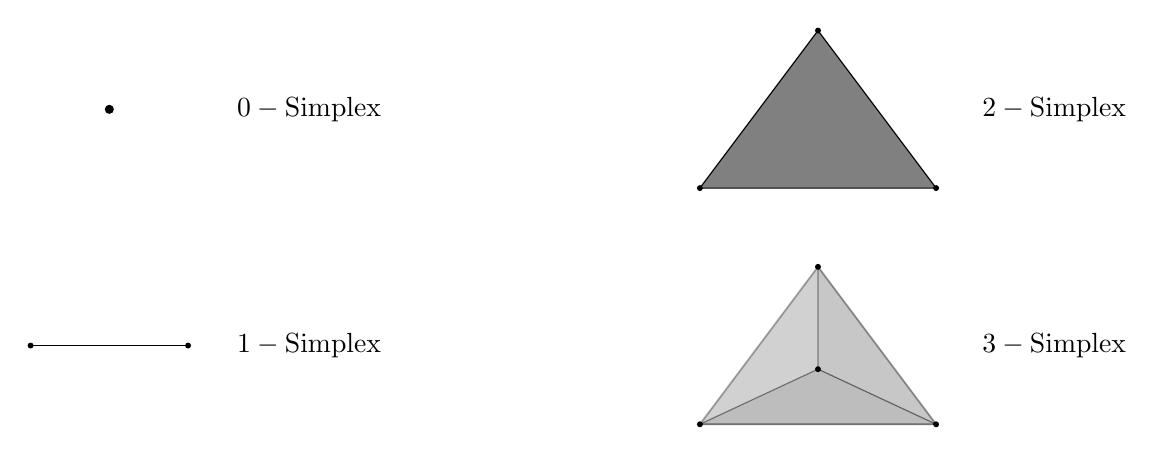
\begin{tikzpicture}
    \node at (1.5,1) [right] {$0-\textrm{Simplex}$};
    \node at (1.5,-2) [right] {$1-\textrm{Simplex}$};
    \node at (12,1) {$2-\textrm{Simplex}$};
    \node at (12,-2) {$3-\textrm{Simplex}$};
    \draw[fill=black] (0,1) circle (0.05);
    \draw[fill=black] (-1,-2) circle (0.03);
    \draw[fill=black] (1,-2) circle (0.03);
    \draw[draw=black] (1,-2) -- (-1,-2);
    \draw[fill=gray] (9,2)--(7.5,0)--(10.5,0)--cycle;
    \draw[fill=black] (9,2) circle (0.03);
    \draw[fill=black] (7.5,0) circle (0.03);
    \draw[fill=black] (10.5,0) circle (0.03);
    \draw[fill=gray,opacity=0.2]
        (9,-1)--(7.5,-3)--(9,-2.3)--cycle;
    \draw[fill=gray,opacity=0.3]
        (9,-1)--(10.5,-3)--(9,-2.3)--cycle;
    \draw[fill=gray,opacity=0.4]
        (9,-2.3)--(7.5,-3)--(10.5,-3)--cycle;
    \draw[fill=gray,opacity=0.2, thick]
        (9,-1)--(7.5,-3)--(10.5,-3)--cycle;
    \draw[fill=black] (9,-1) circle (0.03);
    \draw[fill=black] (7.5,-3) circle (0.03);
    \draw[fill=black] (10.5,-3) circle (0.03);
    \draw[fill=black] (9,-2.3) circle (0.03);
\end{tikzpicture}
            \caption{Examples of Simplices.}
            \label{fig:surgery_theory_simplexes}
        \end{figure}
        A simplicial complex is a set of simplices
        $\mathcal{H}$ such that the face of any element
        of $\mathcal{H}$ is also contained in $\mathcal{H}$,
        and the intersection of two simplices
        $\sigma_{1},\sigma_{2}\in \mathcal{K}$ is a
        face of both $\sigma_{1}$ and $\sigma_{2}$.
        We return to studying surgery exact sequences
        for $n\geq 5$. Let $\mathcal{M}$ be an $n$
        dimensional manifold, and let $G=\pi_{1}(\mathcal{M})$.
        In our surgery exact sequence we still have this
        mysterious object $[\mathcal{M},G/Cat]$. Let Cat
        be either PL or Top. The generalized Poincare
        Conjecture says that, for $n\geq 5$,
        $S^{PL}(S^{n})=S^{Top}(S^{n})=\{S^{n}\}$.
        Let $\mathcal{M}=S^{n}$. Then
        $G=\pi_{1}(\mathcal{M})=\{e\}$.
        Then we have the following:
        \begin{figure}[H]
            \centering
            \captionsetup{type=figure}
            \documentclass[crop,class=article]{standalone}
%----------------------------Preamble-------------------------------%
%---------------------------Packages----------------------------%
\usepackage{geometry}
\geometry{b5paper, margin=1.0in}
\usepackage[T1]{fontenc}
\usepackage{graphicx, float}            % Graphics/Images.
\usepackage{natbib}                     % For bibliographies.
\bibliographystyle{agsm}                % Bibliography style.
\usepackage[french, english]{babel}     % Language typesetting.
\usepackage[dvipsnames]{xcolor}         % Color names.
\usepackage{listings}                   % Verbatim-Like Tools.
\usepackage{mathtools, esint, mathrsfs} % amsmath and integrals.
\usepackage{amsthm, amsfonts, amssymb}  % Fonts and theorems.
\usepackage{tcolorbox}                  % Frames around theorems.
\usepackage{upgreek}                    % Non-Italic Greek.
\usepackage{fmtcount, etoolbox}         % For the \book{} command.
\usepackage[newparttoc]{titlesec}       % Formatting chapter, etc.
\usepackage{titletoc}                   % Allows \book in toc.
\usepackage[nottoc]{tocbibind}          % Bibliography in toc.
\usepackage[titles]{tocloft}            % ToC formatting.
\usepackage{pgfplots, tikz}             % Drawing/graphing tools.
\usepackage{imakeidx}                   % Used for index.
\usetikzlibrary{
    calc,                   % Calculating right angles and more.
    angles,                 % Drawing angles within triangles.
    arrows.meta,            % Latex and Stealth arrows.
    quotes,                 % Adding labels to angles.
    positioning,            % Relative positioning of nodes.
    decorations.markings,   % Adding arrows in the middle of a line.
    patterns,
    arrows
}                                       % Libraries for tikz.
\pgfplotsset{compat=1.9}                % Version of pgfplots.
\usepackage[font=scriptsize,
            labelformat=simple,
            labelsep=colon]{subcaption} % Subfigure captions.
\usepackage[font={scriptsize},
            hypcap=true,
            labelsep=colon]{caption}    % Figure captions.
\usepackage[pdftex,
            pdfauthor={Ryan Maguire},
            pdftitle={Mathematics and Physics},
            pdfsubject={Mathematics, Physics, Science},
            pdfkeywords={Mathematics, Physics, Computer Science, Biology},
            pdfproducer={LaTeX},
            pdfcreator={pdflatex}]{hyperref}
\hypersetup{
    colorlinks=true,
    linkcolor=blue,
    filecolor=magenta,
    urlcolor=Cerulean,
    citecolor=SkyBlue
}                           % Colors for hyperref.
\usepackage[toc,acronym,nogroupskip,nopostdot]{glossaries}
\usepackage{glossary-mcols}
%------------------------Theorem Styles-------------------------%
\theoremstyle{plain}
\newtheorem{theorem}{Theorem}[section]

% Define theorem style for default spacing and normal font.
\newtheoremstyle{normal}
    {\topsep}               % Amount of space above the theorem.
    {\topsep}               % Amount of space below the theorem.
    {}                      % Font used for body of theorem.
    {}                      % Measure of space to indent.
    {\bfseries}             % Font of the header of the theorem.
    {}                      % Punctuation between head and body.
    {.5em}                  % Space after theorem head.
    {}

% Italic header environment.
\newtheoremstyle{thmit}{\topsep}{\topsep}{}{}{\itshape}{}{0.5em}{}

% Define environments with italic headers.
\theoremstyle{thmit}
\newtheorem*{solution}{Solution}

% Define default environments.
\theoremstyle{normal}
\newtheorem{example}{Example}[section]
\newtheorem{definition}{Definition}[section]
\newtheorem{problem}{Problem}[section]

% Define framed environment.
\tcbuselibrary{most}
\newtcbtheorem[use counter*=theorem]{ftheorem}{Theorem}{%
    before=\par\vspace{2ex},
    boxsep=0.5\topsep,
    after=\par\vspace{2ex},
    colback=green!5,
    colframe=green!35!black,
    fonttitle=\bfseries\upshape%
}{thm}

\newtcbtheorem[auto counter, number within=section]{faxiom}{Axiom}{%
    before=\par\vspace{2ex},
    boxsep=0.5\topsep,
    after=\par\vspace{2ex},
    colback=Apricot!5,
    colframe=Apricot!35!black,
    fonttitle=\bfseries\upshape%
}{ax}

\newtcbtheorem[use counter*=definition]{fdefinition}{Definition}{%
    before=\par\vspace{2ex},
    boxsep=0.5\topsep,
    after=\par\vspace{2ex},
    colback=blue!5!white,
    colframe=blue!75!black,
    fonttitle=\bfseries\upshape%
}{def}

\newtcbtheorem[use counter*=example]{fexample}{Example}{%
    before=\par\vspace{2ex},
    boxsep=0.5\topsep,
    after=\par\vspace{2ex},
    colback=red!5!white,
    colframe=red!75!black,
    fonttitle=\bfseries\upshape%
}{ex}

\newtcbtheorem[auto counter, number within=section]{fnotation}{Notation}{%
    before=\par\vspace{2ex},
    boxsep=0.5\topsep,
    after=\par\vspace{2ex},
    colback=SeaGreen!5!white,
    colframe=SeaGreen!75!black,
    fonttitle=\bfseries\upshape%
}{not}

\newtcbtheorem[use counter*=remark]{fremark}{Remark}{%
    fonttitle=\bfseries\upshape,
    colback=Goldenrod!5!white,
    colframe=Goldenrod!75!black}{ex}

\newenvironment{bproof}{\textit{Proof.}}{\hfill$\square$}
\tcolorboxenvironment{bproof}{%
    blanker,
    breakable,
    left=3mm,
    before skip=5pt,
    after skip=10pt,
    borderline west={0.6mm}{0pt}{green!80!black}
}

\AtEndEnvironment{lexample}{$\hfill\textcolor{red}{\blacksquare}$}
\newtcbtheorem[use counter*=example]{lexample}{Example}{%
    empty,
    title={Example~\theexample},
    boxed title style={%
        empty,
        size=minimal,
        toprule=2pt,
        top=0.5\topsep,
    },
    coltitle=red,
    fonttitle=\bfseries,
    parbox=false,
    boxsep=0pt,
    before=\par\vspace{2ex},
    left=0pt,
    right=0pt,
    top=3ex,
    bottom=1ex,
    before=\par\vspace{2ex},
    after=\par\vspace{2ex},
    breakable,
    pad at break*=0mm,
    vfill before first,
    overlay unbroken={%
        \draw[red, line width=2pt]
            ([yshift=-1.2ex]title.south-|frame.west) to
            ([yshift=-1.2ex]title.south-|frame.east);
        },
    overlay first={%
        \draw[red, line width=2pt]
            ([yshift=-1.2ex]title.south-|frame.west) to
            ([yshift=-1.2ex]title.south-|frame.east);
    },
}{ex}

\AtEndEnvironment{ldefinition}{$\hfill\textcolor{Blue}{\blacksquare}$}
\newtcbtheorem[use counter*=definition]{ldefinition}{Definition}{%
    empty,
    title={Definition~\thedefinition:~{#1}},
    boxed title style={%
        empty,
        size=minimal,
        toprule=2pt,
        top=0.5\topsep,
    },
    coltitle=Blue,
    fonttitle=\bfseries,
    parbox=false,
    boxsep=0pt,
    before=\par\vspace{2ex},
    left=0pt,
    right=0pt,
    top=3ex,
    bottom=0pt,
    before=\par\vspace{2ex},
    after=\par\vspace{1ex},
    breakable,
    pad at break*=0mm,
    vfill before first,
    overlay unbroken={%
        \draw[Blue, line width=2pt]
            ([yshift=-1.2ex]title.south-|frame.west) to
            ([yshift=-1.2ex]title.south-|frame.east);
        },
    overlay first={%
        \draw[Blue, line width=2pt]
            ([yshift=-1.2ex]title.south-|frame.west) to
            ([yshift=-1.2ex]title.south-|frame.east);
    },
}{def}

\AtEndEnvironment{ltheorem}{$\hfill\textcolor{Green}{\blacksquare}$}
\newtcbtheorem[use counter*=theorem]{ltheorem}{Theorem}{%
    empty,
    title={Theorem~\thetheorem:~{#1}},
    boxed title style={%
        empty,
        size=minimal,
        toprule=2pt,
        top=0.5\topsep,
    },
    coltitle=Green,
    fonttitle=\bfseries,
    parbox=false,
    boxsep=0pt,
    before=\par\vspace{2ex},
    left=0pt,
    right=0pt,
    top=3ex,
    bottom=-1.5ex,
    breakable,
    pad at break*=0mm,
    vfill before first,
    overlay unbroken={%
        \draw[Green, line width=2pt]
            ([yshift=-1.2ex]title.south-|frame.west) to
            ([yshift=-1.2ex]title.south-|frame.east);},
    overlay first={%
        \draw[Green, line width=2pt]
            ([yshift=-1.2ex]title.south-|frame.west) to
            ([yshift=-1.2ex]title.south-|frame.east);
    }
}{thm}

%--------------------Declared Math Operators--------------------%
\DeclareMathOperator{\adjoint}{adj}         % Adjoint.
\DeclareMathOperator{\Card}{Card}           % Cardinality.
\DeclareMathOperator{\curl}{curl}           % Curl.
\DeclareMathOperator{\diam}{diam}           % Diameter.
\DeclareMathOperator{\dist}{dist}           % Distance.
\DeclareMathOperator{\Div}{div}             % Divergence.
\DeclareMathOperator{\Erf}{Erf}             % Error Function.
\DeclareMathOperator{\Erfc}{Erfc}           % Complementary Error Function.
\DeclareMathOperator{\Ext}{Ext}             % Exterior.
\DeclareMathOperator{\GCD}{GCD}             % Greatest common denominator.
\DeclareMathOperator{\grad}{grad}           % Gradient
\DeclareMathOperator{\Ima}{Im}              % Image.
\DeclareMathOperator{\Int}{Int}             % Interior.
\DeclareMathOperator{\LC}{LC}               % Leading coefficient.
\DeclareMathOperator{\LCM}{LCM}             % Least common multiple.
\DeclareMathOperator{\LM}{LM}               % Leading monomial.
\DeclareMathOperator{\LT}{LT}               % Leading term.
\DeclareMathOperator{\Mod}{mod}             % Modulus.
\DeclareMathOperator{\Mon}{Mon}             % Monomial.
\DeclareMathOperator{\multideg}{mutlideg}   % Multi-Degree (Graphs).
\DeclareMathOperator{\nul}{nul}             % Null space of operator.
\DeclareMathOperator{\Ord}{Ord}             % Ordinal of ordered set.
\DeclareMathOperator{\Prin}{Prin}           % Principal value.
\DeclareMathOperator{\proj}{proj}           % Projection.
\DeclareMathOperator{\Refl}{Refl}           % Reflection operator.
\DeclareMathOperator{\rk}{rk}               % Rank of operator.
\DeclareMathOperator{\sgn}{sgn}             % Sign of a number.
\DeclareMathOperator{\sinc}{sinc}           % Sinc function.
\DeclareMathOperator{\Span}{Span}           % Span of a set.
\DeclareMathOperator{\Spec}{Spec}           % Spectrum.
\DeclareMathOperator{\supp}{supp}           % Support
\DeclareMathOperator{\Tr}{Tr}               % Trace of matrix.
%--------------------Declared Math Symbols--------------------%
\DeclareMathSymbol{\minus}{\mathbin}{AMSa}{"39} % Unary minus sign.
%------------------------New Commands---------------------------%
\DeclarePairedDelimiter\norm{\lVert}{\rVert}
\DeclarePairedDelimiter\ceil{\lceil}{\rceil}
\DeclarePairedDelimiter\floor{\lfloor}{\rfloor}
\newcommand*\diff{\mathop{}\!\mathrm{d}}
\newcommand*\Diff[1]{\mathop{}\!\mathrm{d^#1}}
\renewcommand*{\glstextformat}[1]{\textcolor{RoyalBlue}{#1}}
\renewcommand{\glsnamefont}[1]{\textbf{#1}}
\renewcommand\labelitemii{$\circ$}
\renewcommand\thesubfigure{%
    \arabic{chapter}.\arabic{figure}.\arabic{subfigure}}
\addto\captionsenglish{\renewcommand{\figurename}{Fig.}}
\numberwithin{equation}{section}

\renewcommand{\vector}[1]{\boldsymbol{\mathrm{#1}}}

\newcommand{\uvector}[1]{\boldsymbol{\hat{\mathrm{#1}}}}
\newcommand{\topspace}[2][]{(#2,\tau_{#1})}
\newcommand{\measurespace}[2][]{(#2,\varSigma_{#1},\mu_{#1})}
\newcommand{\measurablespace}[2][]{(#2,\varSigma_{#1})}
\newcommand{\manifold}[2][]{(#2,\tau_{#1},\mathcal{A}_{#1})}
\newcommand{\tanspace}[2]{T_{#1}{#2}}
\newcommand{\cotanspace}[2]{T_{#1}^{*}{#2}}
\newcommand{\Ckspace}[3][\mathbb{R}]{C^{#2}(#3,#1)}
\newcommand{\funcspace}[2][\mathbb{R}]{\mathcal{F}(#2,#1)}
\newcommand{\smoothvecf}[1]{\mathfrak{X}(#1)}
\newcommand{\smoothonef}[1]{\mathfrak{X}^{*}(#1)}
\newcommand{\bracket}[2]{[#1,#2]}

%------------------------Book Command---------------------------%
\makeatletter
\renewcommand\@pnumwidth{1cm}
\newcounter{book}
\renewcommand\thebook{\@Roman\c@book}
\newcommand\book{%
    \if@openright
        \cleardoublepage
    \else
        \clearpage
    \fi
    \thispagestyle{plain}%
    \if@twocolumn
        \onecolumn
        \@tempswatrue
    \else
        \@tempswafalse
    \fi
    \null\vfil
    \secdef\@book\@sbook
}
\def\@book[#1]#2{%
    \refstepcounter{book}
    \addcontentsline{toc}{book}{\bookname\ \thebook:\hspace{1em}#1}
    \markboth{}{}
    {\centering
     \interlinepenalty\@M
     \normalfont
     \huge\bfseries\bookname\nobreakspace\thebook
     \par
     \vskip 20\p@
     \Huge\bfseries#2\par}%
    \@endbook}
\def\@sbook#1{%
    {\centering
     \interlinepenalty \@M
     \normalfont
     \Huge\bfseries#1\par}%
    \@endbook}
\def\@endbook{
    \vfil\newpage
        \if@twoside
            \if@openright
                \null
                \thispagestyle{empty}%
                \newpage
            \fi
        \fi
        \if@tempswa
            \twocolumn
        \fi
}
\newcommand*\l@book[2]{%
    \ifnum\c@tocdepth >-3\relax
        \addpenalty{-\@highpenalty}%
        \addvspace{2.25em\@plus\p@}%
        \setlength\@tempdima{3em}%
        \begingroup
            \parindent\z@\rightskip\@pnumwidth
            \parfillskip -\@pnumwidth
            {
                \leavevmode
                \Large\bfseries#1\hfill\hb@xt@\@pnumwidth{\hss#2}
            }
            \par
            \nobreak
            \global\@nobreaktrue
            \everypar{\global\@nobreakfalse\everypar{}}%
        \endgroup
    \fi}
\newcommand\bookname{Book}
\renewcommand{\thebook}{\texorpdfstring{\Numberstring{book}}{book}}
\providecommand*{\toclevel@book}{-2}
\makeatother
\titleformat{\part}[display]
    {\Large\bfseries}
    {\partname\nobreakspace\thepart}
    {0mm}
    {\Huge\bfseries}
\titlecontents{part}[0pt]
    {\large\bfseries}
    {\partname\ \thecontentslabel: \quad}
    {}
    {\hfill\contentspage}
\titlecontents{chapter}[0pt]
    {\bfseries}
    {\chaptername\ \thecontentslabel:\quad}
    {}
    {\hfill\contentspage}
\newglossarystyle{longpara}{%
    \setglossarystyle{long}%
    \renewenvironment{theglossary}{%
        \begin{longtable}[l]{{p{0.25\hsize}p{0.65\hsize}}}
    }{\end{longtable}}%
    \renewcommand{\glossentry}[2]{%
        \glstarget{##1}{\glossentryname{##1}}%
        &\glossentrydesc{##1}{~##2.}
        \tabularnewline%
        \tabularnewline
    }%
}
\newglossary[not-glg]{notation}{not-gls}{not-glo}{Notation}
\newcommand*{\newnotation}[4][]{%
    \newglossaryentry{#2}{type=notation, name={\textbf{#3}, },
                          text={#4}, description={#4},#1}%
}
%--------------------------LENGTHS------------------------------%
% Spacings for the Table of Contents.
\addtolength{\cftsecnumwidth}{1ex}
\addtolength{\cftsubsecindent}{1ex}
\addtolength{\cftsubsecnumwidth}{1ex}
\addtolength{\cftfignumwidth}{1ex}
\addtolength{\cfttabnumwidth}{1ex}

% Indent and paragraph spacing.
\setlength{\parindent}{0em}
\setlength{\parskip}{0em}
%--------------------------Main Document----------------------------%
\begin{document}
    \begin{tikzpicture}[>=latex,->,scale=1.4]
        \node (a) {$[S^{5},G/Cat]$};
        \node (b) [right=of a] {$0$};
        \node (c) [below=of a] {$\pi_{5}(G/Cat)$};
        \node (d) [right=of c] {$0$};
        \node (e) [left=of c] {$0$};
        \node (f) [above=of a] {$[S^{5},G/Cat]$};
        \node (g) [left= of f] {$S^{Cat}(S^{5})$};
        \node (h) [left= of g] {$L_{6}(\mathbb{Z})$};
        \node (i) at (f -| b) {$L_{5}(\mathbb{Z})$};
        \path (a) edge (b);
        \path (c) edge (d);
        \path (e) edge (c);
        \path (a) edge (c);
        \path (h) edge (g);
        \path (g) edge (f);
        \path (f) edge (i);
        \path (f) edge (a);
        \path (i) edge (b);
    \end{tikzpicture}
\end{document}
            \caption{Diagram for the Surgery Exact Sequence of $S^{5}$.}
            \label{fig:surgery_theory_example_diagram_%
                   for_surgery_exact_sequence}
        \end{figure}
        So, $\pi_{5}(G/Cat)=\{e\}$. This gives us:
        \begin{align*}
            \cdots\rightarrow
            S^{Cat}(S^{6})\rightarrow
            [S^{6},G/Cat]
            &\rightarrow
            L_{6}(\mathbb{Z})\rightarrow\cdots\\
            \cdots
            &\rightarrow{0}\rightarrow\pi_{6}(G/Cat)\rightarrow
            \mathbb{Z}_{2}\rightarrow{0}
        \end{align*}
        So, we have $\pi_{6}(G/Cat)\cong\mathbb{Z}_{2}$.
        In general, $\pi_{n}(G/o)\cong L_{n}(\mathbb{Z})$.
        \begin{theorem}[Wall's Theorem]
            \begin{equation*}
                L_{n}(\mathbb{Z})=
                \begin{cases}
                    \mathbb{Z},&n\equiv{0}\mod{4}\\
                    0,&n\equiv{1}\mod{4}\\
                    \mathbb{Z}_{2},&n\equiv{2}\mod{4}\\
                    0,&n\equiv{3}\mod{4}
                \end{cases}
            \end{equation*}
        \end{theorem}
        All $L$ groups are periodic, and never have odd
        torsion. That is, there is never
        $\mathbb{Z}_{3},\mathbb{Z}_{5}$, etc. Wall groups
        are hard to compute. Whatever $G/Cat$ is, its
        homotopy groups for $n\geq 5$ are known.
        \subsubsection{Principle G-Bundles}
            A few things are needed:
            \begin{itemize}
                \item Map $p:E\rightarrow X$,
                      where $E$ is a total space
                      and $X$ is a base space.
                \item The inverse-image $E_{x}=p^{-1}(\{x\})$
                      is called the fiber over $x$.
                \item $G$ (Group) acts on each $E_{x}$
                      freely and transitively.
                \item $G$ has to act `continuously.'
                      Nearby points are taken to nearby points.
            \end{itemize}
            Then $p:E\rightarrow X$ is a $G-$principle bundle. Freely
            means the only element that fixes everything is the identity.
            \begin{example}
                Take a sphere $S^{n}$ and a projection
                $p:S^{n} \rightarrow \mathbb{RP}^{n}$.
                $\mathbb{RP}^{n}$ is created by glueing
                antipotal points together.
                If $x\in \mathbb{RP}^{n}$, then $p^{-1}(\{x\})$
                consists of $2$ antipotal points in $S^{n}$.
                Now $\mathbb{Z}_{2}=\{0,1\}$
                can act on a sphere.
                $0$ maps $x\mapsto{x}$ and $1$ maps
                $x\mapsto{-x}$.
                Note that $1+1 = 0$, as in $\mathbb{Z}_{2}$.
                Given any point, you can get to another point
                in the fiber. This is trivial in this example
                as there are only two points in the fiber.
                Also only the identity maps a point back
                to itself. This action is free and transitive,
                so $p:S^{n}\rightarrow\mathbb{RP}^{n}$
                is a $\mathbb{Z}_{2}$-principle bundle.
            \end{example}
            Let $M$ be a manifold (Or a space) with dimension $n$ and
            fundamental group $G$. A universal cover $\tilde{M}$ of $M$ includes
            a map $p:\tilde{M}\rightarrow M$ such that $\tilde{M}$ is simply
            connected of dimension $n$, i.e. $\pi_{1}(\tilde{M})=e$, and
            $\forall_{x\in M}$, $p^{-1}(x)$ is a collection of discrete points.
            $\pi_{1}(\mathbb{RP}^{n})=\mathbb{Z}_{2}$ and $S^{n}$ is a universal
            cover of $\mathbb{RP}^{n}$. This might come from a general theory.
            \begin{example}
                Take the circle $S^{1}$.
                $\pi_{1}(S^{1})=\mathbb{Z}$.
                There's a map $p(x)=e^{2\pi{ix}}$ of modulus 1.
                Note that $p^{-1}(0) = \mathbb{Z}$.
                So $p^{-1}(x)$ is just a shift of
                $\mathbb{Z}$ to $\mathbb{Z}+r$.
                Note that $\pi_{1}(\mathbb{R})=e$.
                So $\mathbb{R}$ is a universal cover of $S^{1}$.
            \end{example}
            \begin{example}
                We may think $\mathbb{R}^2$ is a universal
                cover of $S^{2}$, but $S^{2}$ is already
                simply connected. So $p$ is the
                identity map, and the universal cover of $S^{2}$
                is $S^{2}$. All universal covers are
                homotopy equivalent.
            \end{example}
            Let $x\in\mathcal{M}$. Then, for all $z\in p^{-1}(\{x\})$, and for
            all $g\in \pi_{1}(M)$, there is an action $gx\in p^{-1}(x)$. This
            uses the homotopy lifting property. There is an action $G$ on
            $\tilde{\mathcal{M}}$ which preserves the fiber (Takes every element
            of a fiber to the same fiber. It does not mix fibers), is
            transitive, and is free. The map
            $p:\tilde{\mathcal{M}}\rightarrow\mathcal{M}$ is a $\pi_{1}(M)$
            Principal Bundle.
            \subsubsection{Functors}
                Let $F$ be a functor
                $F:\textit{Space}\rightarrow\textit{Groups}$.
                So for all spaces $X$, we have a group $F(X)$.
                There are many such examples:
                \begin{itemize}
                    \begin{multicols}{4}
                        \item Cohomology
                        \item Homology
                        \item K-Theory
                        \item Other Stuff
                    \end{multicols}
                \end{itemize}
                Homology: Take $M$ and triangulate. Take maps from the
                simplicial complex of $M$ to $G$ (Group) (Certain conditions).
                There's an equivalence relation on these maps. That set after
                taking the equivalence relations is the homology: $H_{n}(M,G)$.
                $n$ describes the type of simplicies. If $n>\dim(M)$, then
                $H_{n}(G,M)=0$. $H_{n}(M,G)=\{f:\Delta^{n}\rightarrow G\}$.
                Cohomology is the set $H^{n}(M,G)=[H_{n}(M,G),G]$, that is, the
                \textit{dual}. We want to talk about cohomology. Under special
                conditions there is something called the Brown Representation
                Theorem. Consider Cohomology $H^{n}(M,G)$, with coefficients in
                $G$. Cohomology is Homotopy invariant, that is if $M\cong{N}$,
                then $H^{n}(M,G)\cong H^{n}(N,G)$. The Brown-Representation
                Theorem says that there is a classifying space $BG$ such that,
                for all spaces $M$, there is a one-to-one correspondence between
                $H^{n}(X,G)\leftrightarrow[X,BG]$. In general, if $F$ is a
                functor, then the Brown-Representation Theorem says that there
                is a classifying space $Y$ such that $F(X)$ has a one-to-one
                correspondence with the homotopy classes of maps, $[X,Y]$.
                $F(x)\leftrightarrow[X,Y]$.
                \begin{example}
                    The Eilenberg-MacLane Space $K(G,n)$ has the property that
                    $\forall_{j\ne{n}}$, $\pi_{n}(K(G,n))=G$, and
                    $\pi_{j}(K(G,n))=0$. $K(G,n)$ is the classifying space for
                    cohomology.
                \end{example}
                \begin{theorem}
                    $K(G,n)$ is the classifying space for cohomology. That is,
                    up to homotopy, $H^{n}(X,G)\leftrightarrow[X,K(G,n)]$.
                \end{theorem}
                Let $\textrm{Prin}_{G}(X)$ be the collection
                of $G-$principal bundles on $X$. With a
                certain equivalence relation, it turns out
                the $\textrm{Prin}_{G}(X)$ is a group. So
                $\textrm{Prin}_{G}:\textit{Spaces}\rightarrow%
                 \textit{Groups}$
                is a functor. The Brown-Representation
                Theorem implies that there is a classifying
                space $BG$
                $\textrm{Prin}_{G}\leftrightarrow[X,BG]$.
                \begin{theorem}
                    If $p:E\rightarrow X$ and $p':E'\rightarrow X$
                    are both bundles over $X$, then there exists
                    $p\oplus p':E\oplus E' \rightarrow X$
                    COME BACK TO LATER
                \end{theorem}
            \subsubsection{Grothendique Groupification of Semigroup}
                \begin{definition}
                A semi-group is a group without the
                requirement for invereses.
                \end{definition}
                \begin{example}
                    $\{0,1,2,\hdots\}$ is a semi-group
                    under addition.
                \end{example}
                Let $G$ be a semi-group. Constraint
                $G\times{G}/\sim$.
                $(a,b)\sim(c,d)$ if $a+d=b+c$.
                So, $(2,3)\sim(4,5)\sim(7,8)\sim(-1,0)\equiv -1$.
                The equivalence class of all of these things is
                called $-1$. We still have all of the positive
                integers, $(4,2)\sim(5,3) \sim(6,4) \equiv 2$.
                This process adds all of the negatives. This
                process, called Grothendique Construction on a
                Semi-group creates a group out of a semi-group.
                It is, in a way, the 'smallest' group containing
                the semi-group. The groupification of
                $\{0,1,2,3,\hdots\}$ will be $\mathbb{Z}$.
                \begin{example}
                    What are the vector bundles over a dot?
                    There is $\mathbb{R}^{0}$ (A dot),
                    $\mathbb{R}^{n},\hdots,\mathbb{R}^n,\hdots$
                    There is an operation on this set
                    $\{\mathbb{R}^{n}:n \geq 0\}$. This makes a
                    semi-group, and there is a Grothendique
                    Groupification
                    $G_{r}(\mathbb{Z}_{\geq 0},+)=\mathbb{Z}$
                \end{example}
                Suppose M is a monoid/semigroup.
                Not required to have an inverse but should
                have an identity. For example,
                $(\mathbb{Z}_{\geq 0},+)$ is a monoid.
                Has identity, but no inverse.
                Construct $M\times M=\{(a,b):a,b\in M\}$
                with the operation $(a,b)+(c,d) = (a+c,b+d)$.
                Think of $(a,b)$ as $a-b$. Note that in
                regular math $'3-1'='4-2'$, so we want $(3,1)$
                to equal $(4,2)$. We do this with the
                equivalence rlation $(a,b)\sim (c,d)$ if
                and only if $a+d=b+c$. Let $M\times M/\sim$
                be called $M_{G}$. 
                \begin{theorem}
                    $M_{G}$ is a group.
                \end{theorem}
                \begin{theorem}
                    There is an injection $i:M\rightarrow M_{G}$
                    with the following property:
                \begin{enumerate}
                    \item $i(a)\sim (a,0)\sim(a+1,1)\sim(a+2,2)\sim\hdots$
                \end{enumerate}
                \end{theorem}
                This construction is functorial, so if there are monoids $M,N$
                with a semi-homomorphism $\phi:M\rightarrow N$
                $(\phi(a*b)=\phi(a)*\phi(b))$ (Homomorphism for a semi-group),
                then there is a HM $\phi_{G}:M_{G}\rightarrow N_{G}$ so
                $G(Monoids,Semihomomorphism)\rightarrow (Groups,Homomorphism)$
                is a functor.
            \subsubsection{Suspension}
                Let $X$ and $Y$ be disjoint topological spaces. The wedge
                product $X\vee Y$ is the one-point union of $X$ and $Y$. Take
                $X$, take $Y$, and glue one point together. 
                \begin{theorem}
                    If $X$ and $Y$ are disjoint topological spaces, then
                    $\pi_{1}(X\vee Y)=\pi_{1}(X)\oplus\pi_{1}(Y)$.
                \end{theorem}
                In the same context, the smash product of $X$ and $Y$ is
                $X\wedge Y=X\times Y/(X\vee Y)$. Picture $X=(0,1]$ in the $x$
                axis and $Y=(0,1]$ in the $y$ axis. Then $X\times Y$ is a
                square in the $xy$ plane, and $X\vee Y$ is the $x$ and $y$ axes
                from $0$ to $1$. So $X\wedge Y$ takes all of the points on the
                two axes between $0$ and $1$ and smashes them down to the
                origin.
                \begin{example}
                    $S^{1}\times [0,1]$ is the hollow cylinder, and
                    $S^{1}\vee [0,1]$ is the boundary of the edge of the
                    cylinder (The lid) and the line going down the cylinder
                    parallel with the z-axis (the spine). So $X\wedge Y$
                    smashes down to a cone. This is then homeomorphic
                    to $D^{2}$. 
                \end{example}
                \begin{example}
                    The torus can be visualized by the diagram shown in
                    Fig.~\ref{fig:plane_representation_of_a_torus}.
                    So $T^{2}=S^{1}\times S^{1}$. Using the diagram, we can see
                    that the smash product $S^{1}\wedge S^{1}$ is homotopy
                    equivalent to a sphere.
                \end{example}
                \begin{definition}
                    Let $X$ be a topological space. Then the suspension of $X$,
                    denoted $\Sigma X$, is $S^{1}\wedge X$.
                \end{definition}
                So $\Sigma S^{n}=S^{n+1}$. The usefulness of smash has to do
                with $\pi_{k}(\Sigma X)=\pi_{k-1}(X)$. There's another thing
                called the Freudenthal suspension theorem.
            \subsubsection{Higher Homotopy}
                The fundamental group, which is the first homotopy group,
                is $\pi_{1}(X)$. Ingredients needed:
                \begin{enumerate}
                    \item Topological Space $X$
                    \item A basepoint $x_{0}$
                \end{enumerate}
            \begin{definition}
                The fundamental group of a topological space $X$ about a
                base point $x_{0}$ is the set:
                \begin{equation}
                    \pi_{1}(X)=[(S^{1},\star),(X,\star)]
                              =Hom\big((S^{1},\star),(X,\star)\big)
                              =\{f:S^{1}\rightarrow X:f(x)
                                    =\star\}/\textrm{Homotopy}
                \end{equation}
            \end{definition}
            $\pi_{1}(X)$ is a group using concatenation. Higher homotopy groups:
            \begin{definition}
            $\pi_{n}(X)=[(S^{n},\star),(X,\star)]$
            \end{definition}
            It turns out that $\pi_{n}(X)$ has a certain operation, for
            $n\geq 2$, such that it is an Abelian group. However, $\pi_{1}(X)$
            need not be an Abelian group.
            \begin{example}
                The Klein bottle is an example of a space such that $\pi_{1}(X)$
                is not an Abelian group.
            \end{example}
            The question becomes 'What are the Homotopy groups of sphere?' That
            is, what is $\pi_{m}(S^{n})$? Recall stereographic projection from
            before. Take $S^{n}$ and remove the north pole (The point
            $(0,0,1)$). This can be projected down to $\mathbb{R}^{2}$. This can
            be generalized to $n$ dimensions, and in general
            $S^{n}\setminus\{\textrm{North Pole}\}$ is homeomorphic to
            $\mathbb{R}^{n}$. Now $\mathbb{R}^{n}$ has $0$ homotopy groups
            because it is contractible (Can be smushed down to a point). If
            $m<n$, then we are mapping a small 'sphere' into a big 'sphere.
            \begin{theorem}
                If $n\ne m$, then there is no continuous function $f$ such that
                $f:S^{n}\rightarrow S^{m}$ is surjective.
            \end{theorem}
            Now, if $m<n$, then we map $S^{m}$ into $S^{n}$. But since there is
            no surjective continuous function we can remove a point from
            $S^{n}$, map it down to $\mathbb{R}^{n}$ and then contract. So,
            $\pi_{m}(S^{n})=0$ for all $m<n$. The next case is when $m=n$. There
            are three obvious maps: The constant map, the identity map, and the
            antipotal map. It can be shown that there are, for all $n$,
            countably many maps. So $\pi_{n}(S^{n})=\mathbb{Z}$. Another neat
            little fun fact is that $\pi_{3}(S^{2})=\mathbb{Z}$. (Related to
            Hopf fibration). Now, the suspension theorem says that
            $\pi_{n+1}(\Sigma X)=\pi_{n}(X)$. So
            $\mathbb{Z}=\pi_{3}(S^{2})=\pi_{4}(\Sigma S^4)=\pi_{4}(S^{3})=\pi_{5}(\Sigma S^{3})=\pi_{5}(S^{4})=\hdots$
            so, if $m-n=1$, then $\pi_{m}(S^{n})=\mathbb{Z}$.
            \begin{theorem}
            $\pi_{3}(S^{2})=\mathbb{Z}$
            \end{theorem}
            \begin{theorem}
            If $m-n=1$, and $n\geq 2$, then $\pi_{m}(S^{n})=\mathbb{Z}$
            \end{theorem}
            These are examples of stability theorems, or stability results.
            \subsubsection{Fibrations}
            \begin{definition}
            A fibration is a map between topological spaces that has the homotopy lifting property for every space $X$.
            \end{definition}
            A fibration gives rise to a long exect sequence of homotopy groups
            \begin{align*}
                \pi_{3}(S^{1})\rightarrow\pi_{3}(S^{3})\rightarrow\pi_{3}(S^{2})
                \rightarrow\pi_{2}(S^{1})&\rightarrow\pi_{2}(S^{3})
                \rightarrow\pi_{2}(S^{1})\rightarrow\hdots\\
                &\hdots\rightarrow\pi_{2}(S^{3})\rightarrow\pi_{2}(S^{2})
                \rightarrow\pi_{1}(S^{1})\rightarrow\pi_{1}(S^{3})
                \rightarrow\pi_{1}(S^{2})
            \end{align*}
            We need to know that $\pi_{n}(S^{1})=0$ if $n\geq 2$. An element of $\pi_{n}(S^{1})$ is $f:S^{n}\rightarrow S^{1}$. Stanley owe's me an explanation.
            This becomes:
            \begin{align*}
                0\rightarrow\mathbb{Z}\rightarrow A\rightarrow 0\rightarrow 0\rightarrow\mathbb{Z}\rightarrow\mathbb{Z}\rightarrow 0\rightarrow 0
            \end{align*}
            \subsubsection{Classifying Space}
            If $G$ is a group (discrete or not), then there is a classifying space (Topological space) $BG$ (unique up to homotopy) such that :
            \begin{enumerate}
                \item $\pi_{1}(BG)=G$ and $\pi_{n}(BG)=0$ for all $n\geq 2$.
                \item There is a contractible space $EG$ that is a principle $G$ bundle with a $G$ action such that $BG\simeq EG/G$. $EG\rightarrow BG$.
                \item For all spaces $X$ with a continuous map $f:X\rightarrow BG$, there is a pullback diagram
                \item The correspondence $(X\rightarrow BG)\rightarrow (Y_{f}\downarrow X)$ has the property that, if $f\simeq g$, then $(Y_{f}\downarrow X)\overset{\textrm{Principle G-Bundle}}{=}(Y_{g}\downarrow X)$. This gives a map $[X,BG]\rightarrow Prin_{G}(X)$ which is a bijection.
            \end{enumerate}
            \begin{definition}
            Let $V$ be a finite dimensional vector space over $\mathbb{F}$. We say that $B:V\times V\rightarrow\mathbb{F}$ is symmetric bilinear if:
            \begin{enumerate}
                \item $B(v,v')=B(v',v)$
                \item $B(v+w,v')=B(v,v')+B(w,v')$
                \item $B(\lambda v,w)=\lambda B(v,w)$
            \end{enumerate}
            \end{definition}
            \begin{example}
            Let $A$ be a symmetric real $n\times n$ matrix. Then $B:\mathbb{R}^{n}\rightarrow\mathbb{R}^{n}\rightarrow \mathbb{R}$ given by $B(X,Y) = X^{T}AY$. This $B$ gives rise to a map $Q:V\rightarrow \mathbb{F}$ given by $Q(x)=B(x,x)$.
            \begin{equation*}
                Q(X)=
                \begin{bmatrix}
                    x,y
                \end{bmatrix}
                \begin{bmatrix}
                    2&0\\
                    0&1
                \end{bmatrix}
                \begin{bmatrix}
                    x&y
                \end{bmatrix}=2x^{2}+y^{2}
            \end{equation*}
            Which is a quadratic form.
            \end{example}
    \subsection{Lecture 5: The Wall L-Groups}
        The Wall L-Groups are defined on all commutative rings.
        In fact, there is a functor $L_{n}$ which takes
        commutative rings to groups. Some facts about this:
        \begin{enumerate}
            \item L-Groups are $4$ periodic.
                  For all commutative rings $R$, we have
                  $L_{n}(R)\simeq L_{n+4}(R)$.
                  This is hard to prove.
            \item Surgery theory requires for
                  $R=\mathbb{Z}G$, where $G$ is the
                  fundamental group of the manifold in
                  question, and $\mathbb{Z}G$ is all
                  finite linear combinations of the elements
                  in $G$.
            \item There is a whole theory of computing
                  $L_{n}(R)$ when $R$ is a field,
                  usually denoted $\mathbb{F}$.
            \item Potentially true statement: L-groups
                  only have 2 or 4 torsion, if they have
                  torsion at all. This is hard to prove,
                  as well.
            \item For $G$ equal to the trivial group,
                  $L_{n}(\mathbb{Z}[e])$ we have
                  $L_{n}(\mathbb{Z}[e])%
                   =\begin{cases}%
                        \mathbb{Z},&n\cong{0}(4)\\%
                        0,&n\cong{1}(4)\\%
                        \mathbb{Z}_{2},&n\cong{2}(4)\\%
                        0,&n\cong{3}(4)%
                    \end{cases}$
        \end{enumerate}
        Suppose $\mathcal{M}^{n}$ is a closed
        manifold and $n\geq 5$, and $\pi_{1}(M)=e$.
        Suppose $n=5$. Then:
        \begin{align*}
            L_{6}(\mathbb{Z}[e])
            &\longrightarrow[\mathcal{M},G/Cat]
            \longrightarrow{S^{Cat}}(\mathcal{M})
            \longrightarrow{L_{5}}(\mathbb{Z}[e]\\
            \mathbb{Z}_{2}&\longrightarrow
            [\mathcal{M},G/Cat]
            \overset{f}{\longrightarrow}S^{Cat}(\mathcal{M})
            \longrightarrow{0}
        \end{align*}
        If $n=6$, we have:
        \begin{align*}
            L_{7}(\mathbb{Z}[e])
            &\rightarrow[M,G/Cat]\rightarrow
            S^{cat}(\mathcal{M})\rightarrow L_{6}(\mathbb{Z}[e])\\
            0&\rightarrow [M,G/Cat]
            \overset{g}{\rightarrow}S^{Cat}(\mathcal{M})
            \overset{?}{\rightarrow}\mathbb{Z}_{2}
        \end{align*}
        In the case of $n=4$, there are these
        things called 'Good' groups in which some
        of these results still hold. The
        dimensions can be broken up like this:
        \begin{itemize}
            \item $2$ Completely solved.
            \item $3$ This is Knot Theory.
            \item $4$ Very hard.
            \item $\geq 5$ Surgery Theory.
        \end{itemize}
        How do you classify manifolds?
        \begin{itemize}
            \item In two dimensions the genus
                  (number of wholes) and the
                  orientation (Euler characteristic)
                  gives you everything.
            \item In three dimensions, Thurnston and
                  Perelman did the classification of this.
            \item Four is a big vacuum of unsolved
                  stuff. 'Good' groups come up here.
            \item For every group $G$ there is a
                  manifold $\mathcal{M}$ of dimensions
                  $5$ or greater such that
                  $\pi_{1}(\mathcal{M})=G$
        \end{itemize}
        Let's study $L_{n}(\mathbb{Z}[e])$.
        This is surprisingly hard enough to study.
        The computation of this was known by Brouder,
        but the use of the surgery exact sequences
        wasn't done until Wall (Hence, Wall groups).
        \subsubsection{The Witt Group}
            $L_{0}(\mathbb{Z}[e])$ is equal to something
            called the Witt group $Witt(\mathbb{Z})$.
            First let's talk about the Witt group of fields.
            The Witt group of a field $\mathbb{F}$ is
            the set of symmetric bilinear forms
            $B:V\times{V}\rightarrow\mathbb{F}$
            of finite dimensional vector spaces
            $V$ over $\mathbb{F}$, modulo some
            equivalence relation. So $B$ can be
            represented by some symmetric matrix
            in $M_{n}(\mathbb{F})$ with respect to
            some basis $\{\beta\}$. So if
            $B:V\times{V}\rightarrow\mathbb{F}$
            has matrix $A_{\beta}$ and if
            $D:V\times{V}\rightarrow\mathbb{F}$
            has matrix $A'_{\delta}$,
            then construct the matrix:
            \begin{equation*}
                \tilde{A}=
                \begin{pmatrix}
                    A&0\\
                    0&A'
                \end{pmatrix}_{\beta,\delta}
            \end{equation*}
            Then one can get a Bilinear form
            $B\perp{D}:V\oplus{V}\rightarrow{V}\oplus{V}$
            using this matrix. This is called the
            orthogonal sum. The equivalence relation
            on these Bilinear forms is a bit complicated.
            Consider the matrix:
            \begin{equation*}
                \begin{bmatrix}
                    x&y
                \end{bmatrix}
                \begin{bmatrix}
                    1&0\\
                    0&-1
                \end{bmatrix}
                \begin{bmatrix}
                    x&y
                \end{bmatrix}
                =x^{2}-y^{2}
            \end{equation*}
            This is called a Hyperbolic form $H_{2}(\mathbb{F})$
            \begin{enumerate}
                \item Two forms 
                      $B_{1}:V\times V\rightarrow \mathbb{F}$
                      and $B_{2}:W\times W\rightarrow \mathbb{F}$,
                      with $\dim(V)=\dim(W)$.
                      If $A^{T}[B_{1}]A=[B_{2}]$,
                      then $B_{1}\sim B_{2}$.
                \item We can also write
                      $B_{1}\sim B_{2}$ is
                      $B_{1}%
                       =B_{2}\underset{k}{\perp}H_{2}(\mathbb{F})$.
                      So $H_{2}(\mathbb{F})$ is the $0$
                      element in $Witt(\mathbb{F})$.
                      Note that, since $H_{2}(\mathbb{F})$
                      has dimension $2$,
                      $\dim(B_{1})=\dim(B_{2})\mod{2}$.
                \item What is the inverse of $B_{1}$?
                      It is a form $B_{2}$ for which
                      $B_{1}\perp B_{2}\simeq H_{2}(\mathbb{F})$
            \end{enumerate}
            There is a map, called the signature map,
            of a matrix
            $W(\mathbb{F})\rightarrow%
             L_{0}(\mathbb{Z}[e])\simeq \mathbb{Z}$.
            It is defined for matrices with real eigenvalues.
            It is the number of positive eigenvalues minus
            the number of negative eignvalues.
        \subsubsection{Manifold Structures}
            Let $X$ be a closed manifold. Then a homotopy
            equivalence $f:\mathcal{N}\rightarrow{X}$ is called a
            manifold structure on $X$. Two manifold structures,
            $f_{1}:\mathcal{N}_{1}\rightarrow{\mathcal{M}}$ and
            $f_{2}:\mathcal{N}_{2}\rightarrow{\mathcal{M}}$, are called
            equivalent on $S(X)$ if there is a homeomorphism
            $g:\mathcal{M}\rightarrow\mathcal{N}$ that
            Fig.~\subref{fig:Equivalent_Manifold_Structure_Diagram} is a
            commutative diagram. Since the composition of homeomorphisms
            is a homeomorphism, if $f_{1}:\mathcal{L}\rightarrow{X}$ and
            $f_{2}:\mathcal{M}\rightarrow{X}$ are equivalent manifold structures
            on $X$, and if $f_{2}:\mathcal{M}\rightarrow{X}$
            and $f_{3}:\mathcal{N}\rightarrow{X}$ are equivalent
            manifold structures, then $f_{1}:\mathcal{L}\rightarrow{X}$
            and $f_{3}:\mathcal{N}\rightarrow{X}$ are equivalent manifold
            structures. That is, the diagram shown in
            Fig.~\ref{fig:Equivalent_Manifold_Structure_Diagram} is a
            commutative diagram.
            \begin{figure}[H]
                \captionsetup{type=figure}
                \begin{subfigure}[b]{0.49\textwidth}
                    \centering
                    \captionsetup{type=figure}
                    \includegraphics{images/Commutative_Diagram_001.pdf}
                    \subcaption{Commutative Diagram for Manifold Structures}
                    \label{fig:Equivalent_Manifold_Structure_Diagram}
                \end{subfigure}
                \begin{subfigure}[b]{0.49\textwidth}
                    \centering
                    \captionsetup{type=figure}
                    \includegraphics{images/Commutative_Diagram_002.pdf}
                    \subcaption{Equivalent Manifolds form an
                                Equivalence Relation.}
                    \label{fig:Equivalent_Manifold_Structure_%
                           Diagram_Equivalence_Relation}
                \end{subfigure}
                \label{Commutative Diagrams for Manifold Structures.}
                \label{fig:Commutative_Diagrams_for_Manifold_Structures}
            \end{figure}
    \subsection{Lecture 6: The Brown Representation Theorem}
        A functor $f:\textrm{Spaces}\rightarrow\textrm{Groups}$
        takes a topological space and returns a group. There are
        many examples, such as homology, cohomoloy, and K-Theory.
        Under certain circumstances there is a space
        $B_{\circ{f}}$ such that there is a one-to-one functor
        $f(\mathcal{M})\leftrightarrow[\mathcal{M},B_{\circ{f}}]$,
        where $\mathcal{M}$ is a manifold.
        \begin{example}
            Let $G$ be a group, and $X\in{K}(G,n)$ an
            Eilenberg-MacLane space. This is not usually a
            manifold, but may be a complex, for example.
            As $X\in{K}(G,n)$, we have that
            $\pi_{n}(X)=G$ and, for all $m\ne{n}$,
            $\pi_{m}(X)=0$. THen $K(G,n)$ is the
            $B_{\circ{f}}$, where the $\circ{f}$ is cohomology
            with coefficients in $G$. That is, we have
            $H^{n}(\mathcal{M};G)%
             \leftrightarrow[\mathcal{M},K(G,n)]$
            is a one-to-one mapping.
        \end{example}
        Conside a manifold $\mathcal{M}$ and the semi-group of
        vector bundles $V(\mathcal{M})$ on $\mathcal{M}$
        with $\oplus$ give by the \textit{Whitney Sum}
        (More on that later). The Grothendique construction gives
        us a group $E(\mathcal{M})$ where the elements are vector
        bundles and ``negative,'' vector bundles (Virtual bundels).
        $E$ can then be thought of as a functor from spaces to
        groups: $E:\textrm{Spaces}\rightarrow\textrm{Groups}$.
        There is some sloppiness ahead that will be clarified later.
        There os a space $BO$ such that
        $E(\mathcal{M})\leftrightarrow[\mathcal{M},BO]$
        is a one-to-one mapping. Note that the
        $B_{\circ{f}}$ are classifying spaces. $BO$ is also
        a classifying space. Let $\mathcal{O}(n)$ be the
        set of orthogonal matrices, as defined in a previous
        lecture. $n\times{n}$ matrices such that $A^{T}=A^{-1}$.
        We saw before that there is a natual mapping $\psi_{n}$
        of $\mathcal{O}(n)$ into $\mathcal{O}(n+1)$. We can
        then form the sequence:
        \begin{equation*}
            \mathcal{O}(1)
            \overset{\psi_{1}}{\longrightarrow}
            \mathcal{O}(2)
            \overset{\psi_{2}}{\longrightarrow}
            \mathcal{O}(3)
            \overset{\psi_{3}}{\longrightarrow}
            \mathcal{O}(4)
            \overset{\psi_{4}}{\longrightarrow}
            \cdots
            \mathcal{O}(n)
            \overset{\psi_{n}}{\longrightarrow}
            \cdots
        \end{equation*}
        And define $\mathcal{O}$ to be the
        \textit{direct limit} of this sequence.
        This is a subset of ``infinite'' dimensional
        matrices. Orthogonal matrices act on vector bundles,
        there are ``rotations,'' of the fibers in
        various dimensions. Let $H$ be a vector bundle over
        $\mathcal{M}$. ``Compactify,'' the fibers,
        which are homeomorphic to $\mathbb{R}^{n}$, making
        them now homeomorphic to $S^{n}$. This is, in a way,
        adding a point ``at infinity,'' or performing the
        one point compactification of $\mathbb{R}^{n}$.
        An example is the stereographic projection of the
        sphere onto the plane. The compactification of
        this is adding the ``North Pole,'' which was
        previously ignored as it is projected
        ``to infinity.'' The stereographic projection
        gives a bijection
        $f:S^{n}\setminus\{\textrm{North Pole}\}%
         \rightarrow\mathbb{R}^{n}$.
        We now have the mapping
        $f:\mathbb{R}^{n}\cup\{\infty\}%
         \rightarrow(S^{n}\setminus\{\textrm{North Pole}\})%
         \cup\{\textrm{North Pole}\}=S^{n}$.
        How to we make $\mathbb{R}^{n}\cup\{\infty\}$ into
        a topological space? If
        $\mathcal{U}$ is open in $\mathbb{R}^{n}$, we say
        that it is still open. Moreover, we say that
        $[-\infty,a)=(-\infty,a)\cup\{\infty\}$ and
        $(a,\infty]=(a,\infty)\cup\{\infty\}$ are also
        open sets. The topology on $\mathbb{R}^{n}$ is
        then the topology generated by the three types
        of sets. Compactifying the fibers of a vector bundle
        creates something called a sphere bundle. An
        example is shown in
        Fig.~\ref{fig:Surgery_Theory_%
                  Compactification_of_Vector_Bundle}.
        \begin{figure}
            \centering
            \captionsetup{type=figure}
            %--------------------------------Dependencies----------------------------------%
%   amsfonts                                                                   %
%   tikz                                                                       %
%       arrows.meta                                                            %
%       positioning                                                            %
%       decorations.markings                                                   %
%-------------------------------Main Document----------------------------------%
\begin{tikzpicture}[%
    >=latex,
    line width=0.2mm,
    line cap=round,
    scale=2
]

    % Coordinates for left blob.
    \coordinate (O1) at ( 0.0, 0.0);
    \coordinate (P1) at ( 1.0, 1.0);
    \coordinate (P2) at ( 0.5, 1.5);
    \coordinate (P3) at (-0.5, 2.0);
    \coordinate (P4) at (-1.0, 1.0);
    \coordinate (M1) at ( 0.5, 1.7);

    % Coordinates for right blob.
    \coordinate (O2) at (3.0, 0.0);
    \coordinate (Q1) at (4.0, 1.0);
    \coordinate (Q2) at (3.5, 1.5);
    \coordinate (Q3) at (2.5, 2.0);
    \coordinate (Q4) at (2.0, 1.0);
    \coordinate (M2) at (3.5, 1.7);

    % Squiggle one.
    \coordinate (L1) at (-1.2, 0.2);
    \coordinate (L2) at (-0.5, 1.0);

    % Squiggle two.
    \coordinate (L3) at (-1.0, -0.3);
    \coordinate (L4) at (-0.3,  0.7);

    % Squiggle three.
    \coordinate (L5) at (-0.3, -0.6);
    \coordinate (L6) at ( 0.0,  0.2);

    % Draw the left blob.
    \draw[%
        postaction={decorate},
        decoration={%
            markings,
            mark=at position .85 with 
                {\filldraw circle (1pt) coordinate (a);},
            mark=at position .9 with
                {\filldraw circle (1pt) coordinate (b);},
            mark=at position .95 with
                {\filldraw circle (1pt) coordinate (c);}
        }
    ]     (O1) to [out=0,in=-120]  (P1) to [out=60,in=20]   (P2)
               to [out=-160,in=45] (P3) to [out=-135,in=90] (P4)
               to [out=-90,in=180] cycle;

    % Label the left manifold as M.
    \node at (M1) {$\mathcal{M}$};

    % Draw squiggles through the three points.
    \draw (L1) to [out=70,in=-150] (a)
               to [out=30,in=-135] (L2) node[above] {$\mathbb{R}^{n}$};
    \draw (L3) to [out=45,in=-135] (b)
               to [out=45,in=-120] (L4) node[right] {$\mathbb{R}^{n}$};
    \draw (L5) to [out=90,in=-135] (c)
               to [out=45,in=-150] (L6) node[right] {$\mathbb{R}^{n}$};

    % Draw arrow from Manifold 1 to Manifold 2.        
    \draw[>=Latex, ->, blue, very thick] (1.1, 1.0) to (1.9, 1.0);

    % Draw right blob.
    \draw[%
        postaction={decorate},
        decoration={%
            markings,
            mark=at position .85 with 
                {\filldraw circle (1pt) coordinate (a);},
            mark=at position .9 with
                {\filldraw circle (1pt) coordinate (b);},
            mark=at position .95 with
                {\filldraw circle (1pt) coordinate (c);}
        }
    ]     (O2) to [out=0,in=-120]  (Q1) to [out=60,in=20] (Q2)
               to [out=-160,in=45] (Q3) to [out=-135,in=90] (Q4)
               to [out=-90,in=180] cycle;

    % Label for the 
    \node at (M2) {$\mathcal{M}$};
    \draw (a) arc(30:390:0.13) node[left=4mm] {$S^{n}$};
    \draw (b) arc(45:405:0.13) node[below left=2mm and 3mm] {$S^{n}$};
    \draw (c) arc(70:430:0.13) node[below right=2mm and 1mm] {$S^{n}$};
\end{tikzpicture}
            \caption{Turning a Vector Bundle into a Sphere Bundle.}
            \label{fig:Surgery_Theory_%
                   Compactification_of_Vector_Bundle}
        \end{figure}
        A spherical fibration is a space $\mathcal{M}$
        where at each point $x$, the fiber of $x$ is
        equivalent to a sphere $S^{n}$ and all
        \textit{transition maps} are homotopy equivalent,
        rather than homeomorphic. The collection of all
        spherical fibrations on a manifold $\mathcal{M}$
        is a semigroup. The Grothendique group associated
        with this is denoted $S(\mathcal{M})$. This group
        is a classifying space. So we have that a vector
        bundle on $\mathcal{M}$ gives rise to a spherical
        fibration on $\mathcal{M}$.
        \begin{equation*}
            \underset{\textrm{Vector Bundle}}{[\mathcal{M},BO]}
            \longrightarrow
            \underset{\textrm{Spherical Fibration}}{[\mathcal{M},BG]}
        \end{equation*}
        We have the following diagrams to consider:
        \begin{figure}
            \centering
            \captionsetup{type=figure}
            \includegraphics{images/Commutative_Diagram_005.pdf}
            \caption{Diagrams for the Lifting Propery.}
            \label{fig:Surgery_Theory_Lifting_Property_Diagram}
        \end{figure}
        Given $\varphi$ and $f$, we can form
        $\hat{\varphi}:\mathcal{M}\rightarrow{BO}$ by taking
        the composition, $\hat{\varphi}(x)=(f\circ\varphi)(x)$.
        The lifting problem is, given the central diagram,
        can we find a continuous map
        $\hat{\varphi}:\mathcal{M}\rightarrow{BG}$ such that
        the diagram becomes commutative? The answer is not always.
        The final diagram gives rise to all ``kernels,'' like
        in exactness: $BG/BO\dashrightarrow{BO}\rightarrow{BG}$.
        We thus define $G/O\equiv{BG/BO}$. The homotopy collection
        $[\mathcal{M},G/O]$ ``computes,'' the extent of which a map
        $\psi:\mathcal{M}\rightarrow{B}$ can be ``lifted,'' to
        $\hat{\varphi}:\mathcal{M}\rightarrow{BO}$.
        Loops on $\mathbb{R}^{n}$, that is, continuous functions
        $f:S^{1}\rightarrow\mathbb{R}^{n}$, can be
        contracted to a point. To put another way, no loops
        can wrap around ``holes'' in $\mathbb{R}^{n}$.
        Therefore, $[\mathbb{R}^{n},G/O]$ is a point. For
        more examples, we have
        $[S^{1},G/O]=\pi_{1}(G/O)$, and
        $[S^{n},G/P]=\pi_{n}(G/O)$. In our discussions
        $O$ gives rise to a differentiable manifold $BO$.
        We can replace this with piece-wise linear or
        topological and obtain spaces like
        $BPL$ or $BTop$, respectively.
        From the Poincare Conjecture we have that
        $S^{Top}(S^{n})=S^{PL}(S^{n})=\{e\}$. That is,
        the trivial group. Our Surgery Exact Sequence now
        becomes:
        \begin{align*}
            \cdots\rightarrow{L}_{n+1}(\mathbb{Z}\pi)
            \rightarrow0\rightarrow
            [\Sigma\mathcal{M},G/Top]&\rightarrow
            L_{n}(\mathbb{Z}\pi)\rightarrow
            0\rightarrow\\
            &\rightarrow[\mathcal{M},G/Top]\rightarrow
            L_{n-1}(\mathbb{Z}\pi)\rightarrow\cdots
        \end{align*}
        So $L_{n+1}(\mathbb{Ze}\simeq[S^{n+1},G/Top]%
            =\pi_{n}(G/Top)$,
        therefore $L_{n+1}(G/Top)\simeq{L_{n}(\mathbb{Z}e)}$.
        \par\hfill\par
        \textbf{Learn about Suspending Space, Wall Groups,
                and Grothendique complete of semigroup}
    \subsection{Lecture 1: Singular and Simplicial Homology}
            The fundamental group $\pi_{1}(X)$ is useful for
            studying low dimensional spaces. However, it is poor for
            studying higher dimensional spaces since, for example,
            it is unable to distinguish spheres of dimensions
            $n\geq 2$. The first solution to this is to study
            the homotopy groups $\pi_{n}(X)$. For this, we have
            that $\pi_{i}(X)=0$ for $i<n$, and $\mathbb{Z}$ for
            $i=n$. A drawback is that homotopy groups are
            difficult to compute. The problem of $\pi_{i}(S^{n})$
            is very difficult for when $i>n$. Homology groups,
            $H_{n}(X)$ are one such solution to this difficulty.
            Homology groups share some characteristics with
            homotopy groups. If $X$ is a CW complex, then $H_{n}(X)$
            depends only on the $(n+1)$-skeleton of $X$. Also,
            $H_{i}(S^{n})$ and $\pi_{i}(S^{n})$ are isomorphic for
            $1\leq i\leq n$. One benefit is that $H_{i}(S^{n})=0$
            for $i>n$.
            \subsubsection{Simplicial Homology}
                The torus, projective plane, and Klein bottle can
                be created from a square by identifying opposite
                edges in certain ways. We can divide the square
                into two triangles, meaning these surfaces can by
                built from two triangles and then identifying
                edges. This can be done for all closed polygons
                as well. We can generalize this to $n$ dimensions
                by considering the $n-\textrm{simplex}$, which is
                the convex hull of a set of $n+1$ points in
                $\mathbb{R}^{n}$ that do not lie in an
                $n-\textrm{dimensional}$ hyperplane.
                $n-\textrm{Simplexes}$ are denoted $\Delta^{n}$.
                The interior of $\Delta^{n}$ is denoted
                $\mathring{\Delta}^{n}$. A face of an
                $n-\textrm{simplex}$ is a simplex formed by
                removing one of the vertices from $\Delta^{n}$.
                \begin{definition}
                    A $\Delta-\textrm{Complex}$ on a space $X$ is
                    a set of maps
                    $\sigma_{\alpha}:\Delta^{n}\rightarrow X$
                    such that:
                    \begin{enumerate}
                        \item The restriction
                            $\sigma_{\alpha}|\mathring{\Delta}^{n}$
                            is injected. Each point $x\in X$ is
                            in the image of only one such
                            $\mathring{\Delta}^{n}$.
                        \item Each restriction of $\sigma_{\alpha}$
                            to a face is equal to one of the maps
                            $\sigma_{\beta}:%
                             \Delta^{n-1}\rightarrow X$.
                        \item A set $A\subset X$ is open if and only
                            if $\sigma_{\alpha}^{-1}$ is open in
                            $\Delta^{n}$ for all $\sigma_{\alpha}$.
                    \end{enumerate}
                \end{definition}
                Let $X$ be a $\Delta-\textrm{Complex}$, and let
                $\Delta_{n}(X)$ be the free abelian group whose
                basis is the open $n-\textrm{simplices}$ of $X$.
                Elements of $\Delta_{n}(X)$ are called
                $n-\textrm{chains}$ and can be written as
                $\sum_{\alpha}n_{\alpha}e_{\alpha}^{n}$, where
                $n_{\alpha}$ is an integer.
                \begin{definition}
                    The Boundary Homomorphism
                    $\partial_{n}:%
                     \Delta_{n}(X)\rightarrow\Delta_{n-1}(X)$
                    is the map:
                    \begin{equation*}
                        \partial_{n}(\sigma_{\alpha})=
                        \sum_{i}(-1)^{i}\sigma_{\alpha}|
                        (v_{0},\hdots,v_{i-1},v_{i+1},\hdots,v_{n})
                    \end{equation*}
                \end{definition}
                \begin{theorem}
                    The composition of
                    $\Delta_{n}(X)%
                     \overset{\partial_{n}}{\longrightarrow}%
                     \Delta_{n-1}(X)%
                     \overset{\partial_{n-1}}{\longrightarrow}%
                     \Delta_{n-2}(X)$
                    is zero.
                \end{theorem}
                \begin{definition}
                    The $n^{th}$ simplicial homology group of
                    $X$, denoted $H_{n}^{\Delta}(X)$,
                    is the quotient group
                    $\ker(\partial_{n})/\Ima(\partial_{n+1})$
                    formed from the chain complex
                    $\cdots\longrightarrow\Delta_{n}(X)%
                     \overset{\partial_{n}}{\longrightarrow}%
                     \Delta_{n-1}(X)%
                     \overset{\partial_{n-1}}{\longrightarrow}%
                     \Delta_{n-2}(X)\longrightarrow\cdots$
                \end{definition}
                The triangle on vertices $a,b,c$ can be defined
                by $[a,b,c]$. We have:
                $\partial_{2}([a,b,c])=[b,c]-[a,c]+[a,b]$.
                The negative sign on $[a,c]$ is used to preserve
                orientation. That is, if you start at $b$,
                travel to $c$, then to $a$, and finally loop
                back to $b$, this should be the ``same'' as going
                from $b$ to $c$, then ``negative'' $a$ to $c$, and
                finally $a$ to $b$. Note that then:
                \begin{subequations}
                    \begin{align}
                        \partial_{2}\partial_{1}([a,b,c])
                        &=\partial_{1}\big([b,c]-[a,c]+[a,b]\big)\\
                        &=\partial_{1}\big([b,c]\big)
                        -\partial_{1}\big([a,c]\big)
                        +\partial_{1}\big([a,b]\big)\\
                        &=(b-c)+(c-a)+(a-b)\\
                        &=0
                    \end{align}
                \end{subequations}
                We can perform the same calculation for the tetrahedron:
                \begin{align*}
                    \partial_{3}\partial_{2}\big([a,b,c,d]\big)
                    =&\hspace{0.5em}\partial_{2}\big([b,c,d]\big)
                     -\partial_{2}\big([a,c,d]\big)
                     +\partial_{2}\big([a,b,d]\big)
                     -\partial_{2}\big([a,b,c]\big)\\
                    =&\hspace{0.5em}\big([c,d]-[b,d]+[b,c]\big)
                     -\big([c,d]-[a,d]+[a,c]\big)+\\
                    &\hspace{0.5em}\big([b,d]-[a,d]+[a,b]\big)
                     -\big([b,c]-[a,c]+[a,b]\big)\\
                    =&\hspace{0.5em}0
                \end{align*}
                Given a complex $W$, we look at the following chain:
                \begin{equation*}
                    C_{n+1}\overset{\partial_{n}}{\longrightarrow}
                    C_{n}\overset{\partial_{n-1}}{\longrightarrow}
                    C_{n-1}\overset{\partial_{n-2}}{\longrightarrow}
                    \cdots\longrightarrow
                    C_{2}\overset{\partial_{1}}{\longrightarrow}C_{1}
                \end{equation*}
                Where $\Ima(\partial_{n+1)})\subset\ker(\partial_{n})$
                and $H_{r}^{\Delta}(W)=\ker(\partial_{n})/\Ima(\partial_{n+1})$.
                We call the elements of $\Ima(\partial_{n+1})$
                \textit{boundaries}, and the elements of
                $\ker(\partial_{n})$ \textit{cycles}.
                \begin{example}
                    Let $W=[a,b]$. That is, the line connecting
                    $a$ and $b$. Then $C_{2}=0$ and
                    $C_{1}=\mathbb{Z}\{[a,b]\}\simeq\mathbb{Z}$.
                    But also
                    $C_{0}=\mathbb{Z}\{[a],[b]\}\simeq\mathbb{Z}^{2}$.
                    So we have
                    $0\rightarrow{C_{1}}\rightarrow{C_{0}}\rightarrow0$.
                    Now $\Ima(\partial_{1})\subset\ker(\partial_{0})$,
                    and $\partial_{0}$ is a mapping from
                    $\mathbb{Z}^{2}$ into $0$, and thus the kernel
                    of $\partial_{0}$ is all of $\mathbb{Z}^{2}$.
                    Moreover, since $\partial_{1}$ is a
                    homomorphism, either the image of $\partial_{1}$
                    is $0$ or $\partial_{1}$ is injective. But
                    $\partial_{1}([a,b])=b-a\ne0$, and therefore
                    $\partial_{1}$ is injective. So we have
                    $H_{0}^{\Delta}(W)=\mathbb{Z}^{2}/\mathbb{Z}=\mathbb{Z}$.
                    For $n>0$, $H_{n}^{\Delta}(W)=0$.
                \end{example}
                \begin{example}
                    Let $W=[a,b,c]$, a triangle including it's interior.
                    Then $C_{3}=0$ and
                    $C_{2}=\mathbb{Z}\{[a,b,c]\}\simeq\mathbb{Z}$.
                    Also $C_{1}=\mathbb{Z}\{b-a,c-a,c-b\}=\mathbb{Z}^{3}$.
                    $\partial_{2}$ is not the zero mapping, and thus
                    $\Ima(\partial_{2})=\mathbb{Z}$. Also $\ker(\partial_{2})=0$,
                    and thus $H_{2}^{\Delta}(W)=0/0=0$. For $\partial_{1}$ we have
                    $\partial_{1}([b,c])=\partial_{1}([a,c])-\partial_{1}([a,b])$,
                    and thus $\Ima(\partial_{1})=\mathbb{Z}^{2}$. But then
                    $\ker(\partial_{1})=\mathbb{Z}$. Therefore
                    $H_{1}^{\Delta}(W)=\mathbb{Z}/\mathbb{Z}=0$.
                    Finally, $\partial_{0}$ is the zero mapping, and
                    thus the kernel is $\ker(\partial_{0})=\mathbb{Z}^{3}$.
                    Therefore
                    $H_{0}^{\Delta}(W)=\mathbb{Z}^{3}/\mathbb{Z}^{2}=\mathbb{Z}$
                \end{example}
                \begin{example}
                    Let $W=\{[a,b],[b,c],[a,c]\}$, a triangle without
                    its interior. Then we have that $C_{2}=0$ and
                    $C_{1}=\mathbb{Z}\{[a,b],[b,c],[a,c]\}=\mathbb{Z}^{3}$.
                    $\partial_{2}$ is the zero mapping and thus
                    $\Ima(\partial_{2})=0$. From the previous example
                    we saw that $\Ima(\partial_{1})=\mathbb{Z}^{2}$,
                    and thus $\ker(\partial_{1})=\mathbb{Z}$.
                    Thus $H_{1}^{\Delta}(W)=\mathbb{Z}/0=\mathbb{Z}$.
                    Finally,
                    $H_{0}^{\Delta}(W)=\mathbb{Z}^{3}/\mathbb{Z}^{2}=\mathbb{Z}$.
                \end{example}
                We see that removing the interior of the triangle changed what
                the homology groups are. As will be seen later, the homology
                groups are way of determining what the ``holes,''
                of the space are.
                \begin{example}
                    Let $W$ be the union of a triangle $[a,b,c]$
                    and a line segment $[c,d]$. Then $C_{3}=0$, and
                    $C_{n}=0$ for all $n>3$. The chain is then
                    $0\rightarrow{C_{2}}\rightarrow{C_{1}}\rightarrow{C_{0}}$.
                \end{example}
                \begin{theorem}
                    If $W$ is contractible and connected,
                    then $H_{0}^{\Delta}(W)=\mathbb{Z}$ and, for all
                    $n>0$, $H_{n}^{\Delta}(W)=0$.
                \end{theorem}
            \subsubsection{Singular Homology}
                Singular homology is formed in the same way that
                simplicial homology is, with the requirement
                that the chains be formed by $\Delta_{n}(X)$ being
                relaxed. Now, only the continuity of the $\sigma$
                are required. Therefore, when $X$ is a space that can
                be ``triangulated,'' we have that the simplicial
                and singular homologies are the same.
                Suppose X and Y are orientable mans f:X-Y continuous. Whats degree?
                Take the nth top homology, $h_n(Z)-h_n(Y,Z)$. This is the map
                $f^*$ which is induced by $f$. Each one of these is a copy of
                $\mathbb{Z}$. So each one of these is a homomorphism. So it has
                to send the number $1\in\mathbb{N}$ somewhere. So the image of
                $1$ is the degree of the map $f$. For example
                $f$ constant, the degree is 0. If $f$ is the identity,
                then the degree is 1. If you take a loop that wraps around
                $S^{1}$ twice then the degree is $2$.
                This looks like the winding number, but is not quite that.